\documentclass[a4paper, 10pt, twoside, openany]{book} % draft

\usepackage[margin=3cm, bindingoffset=1cm]{geometry} % ca. 100pt total margin

\usepackage[perpage]{footmisc}

\usepackage[utf8]{inputenc}

\usepackage[ngerman]{babel}
\hyphenation{Wig-ner}

\usepackage[math]{iwona}
\usepackage{inconsolata}
\usepackage[T1]{fontenc}

\usepackage{amsfonts, amsmath, amssymb, slantsc, mathtools, nicefrac, graphicx, url}

\usepackage[labelfont=bf, font=small, parindent=0.5cm]{caption}
\usepackage[labelfont=bf, font=normalsize, parindent=0.5cm]{subcaption}

\setlength{\marginparwidth}{2.5cm}

\pdfsuppresswarningpagegroup=1

% rules for floats:

\setcounter{topnumber}{1}
\setcounter{bottomnumber}{2}

\def \textfraction {0.1}
\def \topfraction {0.9}
\def \bottomfraction {0.9}
\def \floatpagefraction {0.7}

% source code listings:

\usepackage{listings, color}

\definecolor{grey}{rgb}{0.5, 0.5, 0.5}
\definecolor{dark}{rgb}{0.0, 0.0, 0.5}

\lstset{
  	texcl = true,
	escapebegin = \normalfont \normalsize \,,
	escapeend = \endgraf,
	commentstyle = \color{black},
	%
	basicstyle = \color{dark} \tt \small,
	keywordstyle = \color{blue},
	identifierstyle = \color{black},
	%
	numbers = left,
	numbersep = 0.5cm,
	numberstyle = \color{grey} \tiny,
	%
	showstringspaces = false,
	%
	aboveskip = 0cm,
	belowskip = 1cm,
	}

\lstdefinelanguage{JavaScript}{
	keywords = {break, case, class, catch, const, continue, debugger, default, delete, do, else, export, extends, finally, for, function, if, import, in, instanceof, let, new, return, super, switch, this, throw, try, typeof, var, void, while, with, yield},
	comment = [l]{//},
	morecomment = [s]{/*}{*/},
	string = [b]',
	morestring = [b]",
	sensitive = true,
	}

\makeatletter
	\def \mainmatter {\clearpage \@mainmattertrue \pagenumbering{arabic}}
\makeatother

\newcommand \codesection[1]{\begin{minipage}{0.9\textwidth} \subsection{#1} \end{minipage}}

% headings:

\usepackage{fancyhdr}
\pagestyle{fancy}

\fancyhf{}

\renewcommand \chaptermark[1]{\markboth{\thechapter \quad \MakeUppercase{#1}}{}}
\renewcommand \sectionmark[1]{\markright{\MakeUppercase{#1} \quad \thesection}}

\fancyhead[LE]{\leftmark}
\fancyhead[RO]{\rightmark}
\fancyfoot[C]{\thepage}

\def \headrulewidth {0pt}
\def \footrulewidth {0pt}

\setlength{\headheight}{12.13002pt}

\usepackage[hidelinks]{hyperref}

\newcommand \bra[1]{\left \langle #1 \right |}
\newcommand \ket[1]{\left | #1 \right \rangle}
\newcommand \bracket[2]{\left \langle #1 \middle | #2 \right \rangle}

\newcommand \parens[1]{\left ( #1 \right )}
\newcommand \bracks[1]{\left [ #1 \right ]}
\newcommand \braces[1]{\left \lbrace #1 \right \rbrace}

\newcommand \av[1]{\left \langle #1 \right \rangle}
\newcommand \norm[1]{\left \| #1 \right \|}
\newcommand \abs[1]{\left | #1 \right |}
\newcommand \floor[1]{\left \lfloor #1 \right \rfloor}
\newcommand \ceil[1]{\left \lceil #1 \right \rceil}

\def \I {\mathrm i}
\def \E {\mathrm e}
\def \D {\mathrm d}

\def \mod {\bmod}

\def \phi {\varphi}
\def \epsilon {\varepsilon}
\def \vec {\boldsymbol}

\DeclareMathOperator \sgn {sgn}

\newcommand \op[1]{\mathrm{#1}}

\newcommand \mat[1]{\begin{pmatrix} #1 \end{pmatrix}}
\newcommand \xmat[1]{\begin{Bmatrix} #1 \end{Bmatrix}}

\newcommand \diff[2]{\frac{\D #1}{\D #2}}
\newcommand \pdiff[2]{\frac{\partial #1}{\partial #2}}

\newcommand \veq[2]{\underbrace{#1}_{\displaystyle \mathclap{#2}}}

\def \eC {\varepsilon_\mathrm{C}}
\def \eX {\varepsilon_\mathrm{X}}
\def \nC {n_\mathrm{C}}
\def \nX {n_\mathrm{X}}
\def \nE {n_\mathrm{e}}
\def \cE {c_\mathrm{e}}
\def \cX {c_\mathrm{X}}

\newcommand \src[6][!]{\bibitem[\textsc{#2}]{#3} \textsc{#4}\ifx!#1\else\ #1\fi: \emph{#5}. #6}

\begin{document}
	\frontmatter
	
	\newgeometry{margin = 3cm}
	
	\begin{titlepage}
		\centering
		
		\normalsize
		
\includegraphics[width=5cm]{Abbildungen/Uni.pdf} \hfill 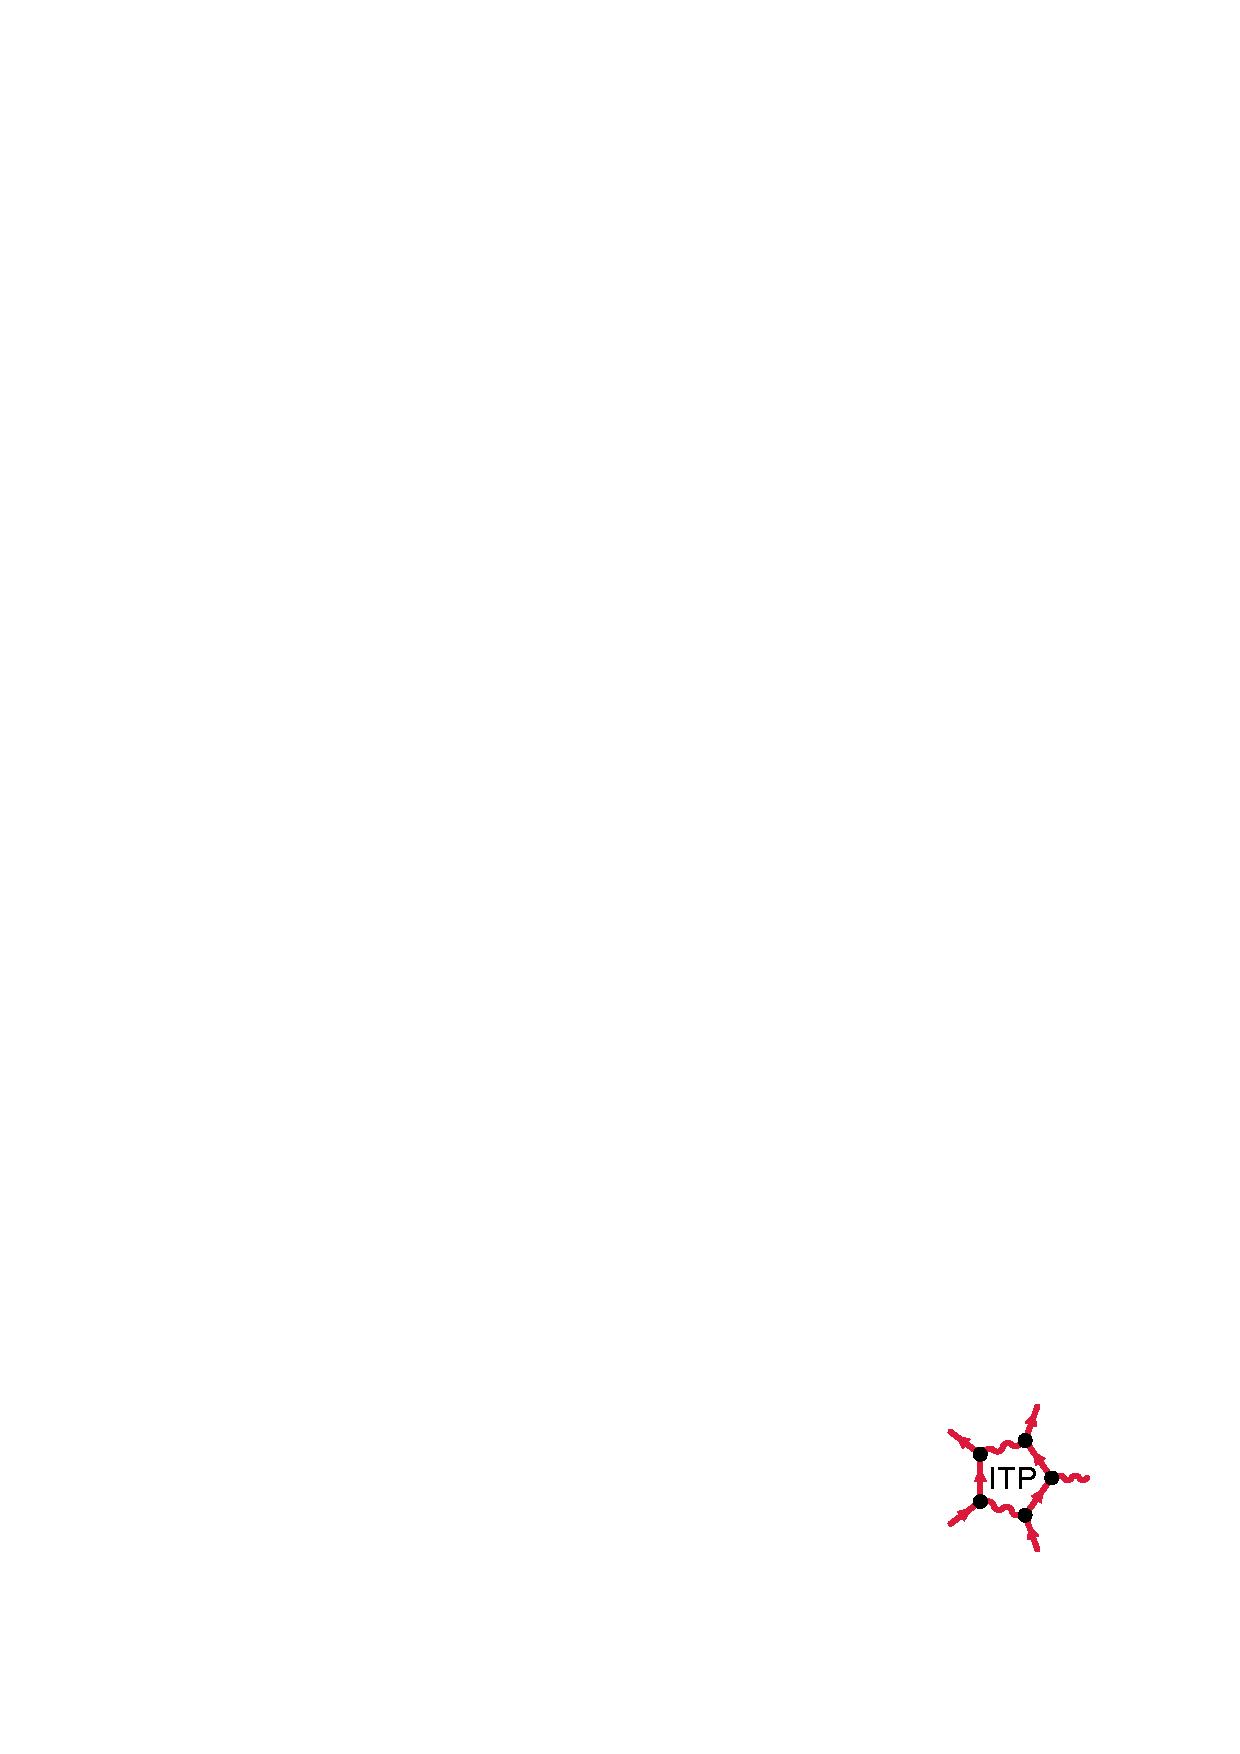
\includegraphics[height=1.5cm]{Abbildungen/ITP.pdf} \\
		\hfill Institut für Theoretische Physik \\
		\hfill \emph{Electronic Structure and Correlated Nanosystems}
		
		\vfill
		
		\Large
		Bachelorarbeit \\[3pc]
		
		\bf \Huge
		Phasen ladungsabhängiger Adsorbatstrukturen auf Graphen \\[3pc]
		
		\it \normalsize
		Phases of charge-dependent adsorbate structures on graphene
		
		\vfill
		
		\normalfont \large
		\hspace{0cm}\llap{vorgelegt von}\hspace{1pc}\rlap{Jan Berges} \\[1pc]
		\hspace{0cm}\llap{Erstgutachter}\hspace{1pc}\rlap{Prof. Dr. Tim Wehling} \\
		\hspace{0cm}\llap{Zweitgutachter}\hspace{1pc}\rlap{Dr. Bálint Aradi} \\[2pc]
		
		4.~September 2014
		
		\vfill
	\end{titlepage}
	
	\newgeometry{left = 4cm, right = 4cm, top = 3cm, bottom = 3cm}
	
	\tableofcontents
	
	\vfill
	
	\begin{flushright}
		\footnotesize
		Gesetzt in Iwona und \texttt{Inconsolata}
	\end{flushright}
	
	\restoregeometry
	
	\mainmatter
	
	\chapter{Motivation}
	
	\begin{figure}[t]
		\begin{minipage}[b]{0.46\textwidth}
			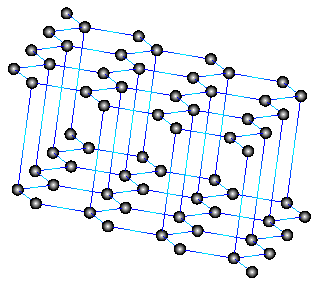
\includegraphics[width=\textwidth]{Abbildungen/Raumstrukturen/Graphit.pdf}
			\caption[Kristallstruktur von Graphit]{Kristallstruktur von Graphit: gegeneinander verschobene Graphenschichten, die nur durch die schwachen \textsc{van-der-Waals}-Kräfte zusammengehalten werden. \cite{Rozplocha}}
			\label{Graphit}
		\end{minipage}
		\hfill
		\begin{minipage}[b]{0.5\textwidth}
			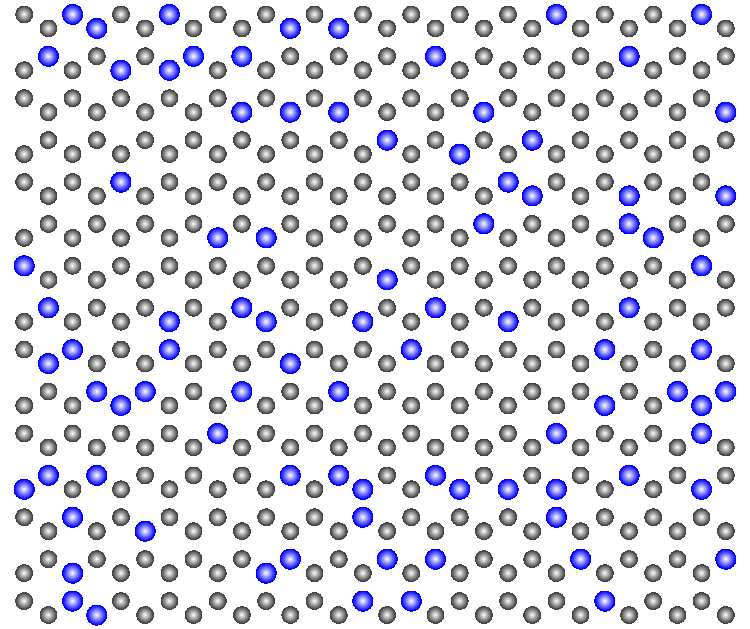
\includegraphics[width=\textwidth]{Abbildungen/random20.pdf}
			\caption[Beispielhafte zufällige Adsorbatkonfiguration auf Graphen]{Beispielhafte zufällige Adsorbatkonfiguration auf Graphen: Die Deckungsrate bzw. Adsorbatkonzentration beträgt 20 Prozent. Bei jedem Kohlenstoffatom (grau) kann sich maximal ein Fremdatom (blau) befinden. Die genaue Geometrie der Bindung wird in diesem Modell nicht berücksichtigt.}
			\label{random20}
		\end{minipage}
	\end{figure}
	%
	Nachdem es der Arbeitsgruppe um \textsc{Konstantin Novoselov} und \textsc{Andre Geim} im Jahr 2004 gelang entgegen vieler Erwartungen die Stabilität einzelner einatomiger Schichten von Graphit (siehe Abb.~\ref{Graphit}) nachzuweisen,\footnote{\emph{"`Planar graphene itself has been presumed not to exist in the free state \emph{[\dots]}. We have been able to prepare graphitic sheets of thicknesses down to a few atomic layers (including single-layer graphene) \emph{[\dots]}."'} \cite[S.~666f]{Novoselov1}} erregte \emph{Graphen} auf Grund seiner außergewöhnlichen Eigenschaften\footnote{In seiner Nobelpreisrede im Jahr 2010 nennt \textsc{Novoselov} eine Vielzahl von Superlativen, darunter die extreme Elastizität und absolute Undurchlässigkeit des sowohl dünnsten als auch stärksten bekannten Materials. \cite[S.~107]{Novoselov2}} große Aufmerksamkeit.
	
	Wie gezeigt werden wird, befindet es sich genau auf der Grenze zwischen Metall und Halbleiter. Die wenigen Elektronen bzw. Löcher, die sich im Bereich des \textsc{Fermi}-Niveaus befinden, weisen zudem eine lineare Dispersion auf und damit ein Verhalten, das vergleichbar ist mit dem vermeintlicher masseloser Fermionen laut der \textsc{Dirac}-Gleichung.\footnote{siehe dazu \cite[Abschnitt III]{Katsnelson2}} Andererseits lässt sich durch flächendeckende Adsorption von Wasserstoff der Isolator \emph{Graphan} erzeugen,\footnote{\emph{"`Particularly elegant is the idea of attaching atomic hydrogen to each site of the graphene lattice to create graphane, \emph{[\dots]} thus removing the conducting $\pi$-bands and opening an energy gap."'} \cite[S.~610]{Elias}} während ladungsdotiertem Graphen sogar Supraleitfähigkeit zugeschrieben wird.\footnote{Eine entsprechende Vorhersage wurde 2012 von einer Gruppe um \textsc{Nandkishore} \cite{Nandkishore} getroffen.} Im Bereich der chemischen Funktionalisierung gibt es also viel Spielraum.
	
	In dieser Hinsicht ist es ein großer Vorteil der Zweidimensionalität von Graphen, dass jedes Kohlenstoffatom von zwei Seiten aus direkt zugänglich ist, im Gegensatz zu gewöhnlichen dreidimensionalen Festkörpern, deren Oberfläche nur einen verschwindenden Anteil der Gesamtzahl aller Atome ausmacht. So ist es beispielsweise möglich von der einen Seite aus mit Ladung zu dotieren\footnote{etwa über das Zusammenspiel von $\rm SiO_2$-Substrat und Wasser, siehe \cite{Wehling1}} und gleichzeitig auf der anderen gezielt Fremdatome anzulagern. Es ist diesbezüglich bekannt, dass für gegebene Ladungsträger- und Adsorbatkonzentrationen spezielle Adsorbatkonfiguationen charakteristisch bzw. energetisch günstig sind.\footnote{Ausgangspunkt der vorliegenden Arbeit sind im Wesentlichen die Ergebnisse von \cite{Wehling2}.}
	
	\textsc{Born} und \textsc{Oppenheimer} folgend, dass sich die elektronische Struktur in erster Näherung als Konsequenz der atomaren betrachten lässt,\footnote{\emph{"`\emph{[\dots]}; der größte Beitrag rührt von der Elektronenbewegung um die Kerne her, \emph{[\dots]}."'} \cite[S.~457]{Born}} werden in dieser Arbeit entsprechende Konfigurationen (siehe Abb.~\ref{random20}) für Wasserstoff und Fluor ermittelt um schließlich vollständige Phasendiagramme zu erhalten. Verwendung findet dabei ein einfaches \emph{Tight-Binding-Modell} in Verbindung mit einem heuristischen Optimierungsverfahren, dem sogenannten \emph{Hill-Climbing-Algorithmus}. Zur quantitativen Charakterisierung der auftretenden Phasen werden zudem verschiedene beschreibende Größen definiert.
	
	Um die direkten Auswirkungen von Veränderungen der Adsorbatstruktur am Rechner untersuchen zu können sind geeignete Ein- und Ausgabemethoden vonnöten. Zu diesem Zweck wurde im Rahmen dieser Arbeit eine grafische Benutzeroberfläche programmiert. Diese ermöglicht neben der Eingabe unterschiedlicher Modellparameter und dem Aufruf der implementierten Algorithmen ein manuelles Arrangieren der Fremdatome bei gleichzeitiger Anzeige der resultierenden Zustandsdichten und Phasendiagramme.
	
	Im folgenden Kap.~\ref{Theorie} werden zunächst einige Grundlagen der Festkörper- und statistischen Physik erläutert, auf denen die weitere Arbeit basiert, deren Ergebnisse in Kap.~\ref{Ergebnisse} dargestellt sind. Nach der Zusammenfassung und einem Ausblick sind im Anhang weitere Abbildungen sowie eine Auflistung verwendeter Quelltexte samt ausführlicher Beschreibung zu finden. Eine lauffähige Version des Programms ist derzeit im Internet unter der Adresse \url{http://berges.canopus.uberspace.de/graphene} abrufbar. Dort sind zudem alle Phasendiagramme und Adsorbatkonfigurationen zu finden, die für diese Arbeit berechnet wurden.
	
    \chapter{Physikalische Grundlagen}
	\label{Theorie}
	
	Hier werden die physikalischen Modelle, Schreibweisen und Methoden, die im weiteren Verlauf der Arbeit Verwendung finden, vorgestellt. Nach einer Abhandlung der festkörpertheoretischen Grundlagen einschließlich des Tight-Binding-Modells wird thermodynamisch die Suche nach "`energetisch günstigen"' Strukturen motiviert, jeweils in direktem Bezug auf den Gegenstand dieser Arbeit. Den Abschluss bildet eine Einführung in die Theorie der Phasenübergänge, wobei hauptsächlich auf die Klassifikation nach \textsc{Ehrenfest} eingegangen wird.
	
	\section{Atomare Struktur}
	\label{Atomare Struktur}
	
	\subsection{\textsc{Bravais}-Gitter und \textsc{Voronoi}-Diagramm}
	\label{Bravais-Gitter}
	
	Unter Vernachlässigung thermischer Effekte ist Graphen eine ideal wabenförmige Anordnung von Kohlenstoffatomen, wobei der Abstand nächster Nachbarn bzw. die Kantenlänge eines Sechsecks jeweils $a \approx 1.42 \cdot 10^{-10}\,\mathrm{m}$ beträgt.\footnote{laut \cite[S.~6]{Katsnelson1}} Eine \emph{Elementarzelle}, d.h. der kleinstmögliche Bereich, der sich periodisch über den gesamten Kristall hinweg fortsetzt, umfasst jeweils zwei Atome, die sogenannte \emph{Basis}. Ihr Flächeninhalt $A = 1.5 \sqrt{3} a^2$ gleicht sowohl dem eines der Sechsecke als auch dem der Raute, die von den beiden Translationsvektoren $\vec t_1$ und $\vec t_2$ aufgespannt wird, die das System auf sich selbst abbilden. Diese stehen in einem Winkel von $60^\circ$ bzw. $120^\circ$ zueinander und haben die Länge $\sqrt 3 a$ gemein. Eine mögliche Wahl in kartesischen Koordinaten $(x \ y)$ mit $\vec t_1$ parallel zur $x$-Achse ist das Rechtssystem\footnote{In einem \emph{Rechtssystem} liegt der jeweils nächste Vektor \emph{links} von seinem Vorgänger (vgl. rechte Hand), wird also auf kürzestem Wege durch eine Drehung entgegen dem Uhrzeigersinn erreicht.}
	%
	\begin{figure}
		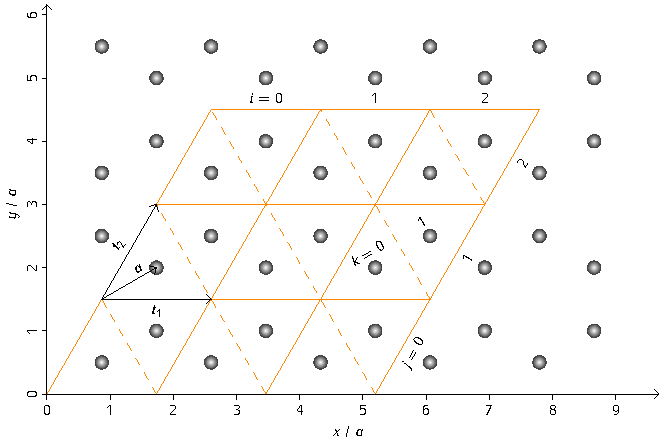
\includegraphics[width=\textwidth]{Abbildungen/Raumstrukturen/Orientierung.pdf}
		\caption[Orientierung im Wabengitter]{Beziehung zwischen den Realraumkoordinaten $(x \ y)$ und dem Koeffiziententripel $(i \ j \ k)$ über die Translationsvektoren $\vec t_1$, $\vec t_3$ und $\vec a$. Für eine Superzelle mit $l = 3$ sind die durch das \textsc{Bravais}-Gitter definierten Elementarzellen mit durchgezogenen orangen Linen markiert, die zusammen mit den gestrichelten das \textsc{Voronoi}-Diagramm der Atome darstellen.
		
		In anderen Abbildungen wird eine rechteckige Darstellung der Superzelle gewählt, wobei der "`Überhang"' der Raute auf der rechten Seite abgeschnitten, dafür aber die entsprechende Lücke bis zur $y$-Achse aufgefüllt wird. Bei der periodischen Fortsetzung in vertikaler Richtung ist dann ein horizontaler Versatz zu berücksichtigen.}
		\label{Orientierung}
	\end{figure}
	%
	\begin{align*}
		\vec t_1 = \mat{\sqrt 3 a \\ 0} \quad \text{und} \quad \vec t_2 = \sqrt{3} a \mat{\cos 60^\circ \\ \sin 60^\circ} = \frac a 2 \mat{\sqrt 3 \\ 3}.
	\end{align*}
	%
	Wenn man des Weiteren die Knotenpunkte bzw. Gittervektoren $\vec R = i \vec t_1 + j \vec t_2$ mit $i, j \in \mathbb Z$ des \emph{\textsc{Bravais}-Gitters} in die Mittelpunkte der Sechsecke legt, erhält man eine Anordnung wie in Abb.~\ref{Orientierung}. Mit dem Untergitterindex $k \in \braces{0, 1}$ zur Unterscheidung der beiden Basisatome sind die Atompositionen gegeben durch
	%
	\begin{align*}
		\vec C = \smash{\overbrace{i \vec t_1 + j \vec t_2}^{\vec R}} + (k + 1) \vec a, \quad \text{wobei} \quad \vec a = a \mat{\cos 30^\circ \\ \sin 30^\circ} = \frac a 2 \mat{\sqrt 3 \\ 1}
	\end{align*}
	%
	jeweils von $\vec R$ zum ersten Basisatom bzw. vom diesem zum zweiten zeigt. Umgekehrt lässt sich wegen der linearen Unabhängigkeit von $\vec t_1$ und $\vec t_2$ sowie der Beschränktheit von $k$ jedem Atom nun eindeutig ein ganzzahliges Tripel $(i \ j \ k)$ zuweisen, das oft einfacher zu handhaben ist.
	
	Für eine rautenförmige \emph{Superzelle}, also einen entsprechenden Gitterausschnitt mit periodischen Randbedingungen, bestehend aus jeweils $l$ Zeilen and Spalten von Elementarzellen und damit $\nC = 2 l^2$ Kohlenstoffatomen, weisen die expliziten Ausdrücke
	%
	\begin{align}
		\begin{aligned}
			i &= \floor{\tilde i \mod l} \\
			j &= \floor{\tilde j \mod l} \\
			k &= \floor{\tilde i \mod 1 + \tilde j \mod 1}
		\end{aligned}
		\qquad \text{mit} \qquad
		\begin{aligned}
			\tilde i &= \frac 1 a \bracks{\frac x {\sqrt 3} - \frac y 3} \\
			\tilde j &= \frac{3 y}{2 a}
		\end{aligned}
		\label{ijk}
	\end{align}
	%
	jedem Punkt $(x \ y)$ das Tripel $(i \ j \ k)$ des jeweils nächstgelegenen Atoms zu und damit die Zugehörigkeit zu dessen \emph{\textsc{Voronoi}-Region},\footnote{Die nach dem ukrainischen Mathematiker benannten \textsc{Voronoi}-Diagramme unterteilen den Raum in "`Einzugsgebiete"' ausgewählter Punkte bzgl. der kürzesten euklidischen Distanz. \cite[S.~10]{Edelsbrunner}} die hier gerade genau eine halbe Elementarzelle darstellt.
	
	Im Gegensatz dazu erfüllen die \textsc{Voronoi}-Regionen der \textsc{Bravais}-Gitterpunkte, \emph{\textsc{Wigner-Seitz}-Zellen} genannt, die Definition für Elementarzellen und sind hier deckungsgleich mit den Sechsecken des Wabenmusters.
	
	Einfach ist mit Hilfe der $(i \ j \ k)$ auch die explizite Angabe der drei nächsten Nachbarn eines Kohlenstoffatoms der Superzelle:
	%
	\begin{align*}
	    \begin{array}{r c l c r}
			& & ((i + 2 k - 1) \mod l & j & 1 - k) \\
			& \nearrow & & & \\
			(i \ j \ k) & \rightarrow & (i & (j + 2 k - 1) \mod l & 1 - k) \\
			& \searrow & & & \\
			& & (i & j & 1 - k)
		\end{array}
	\end{align*}
	
	\subsection[Reziprokes Gitter und \textsc{Fourier}-Reihen]{Reziprokes Gitter und \textsc{Fourier}-Reihen\footnote{Dieser Abschnitt hält sich stark an Kapitel 1.3 "`Periodische Funktionen"' des Lehrbuchs von \textsc{Czycholl} \cite[S.~18f]{Czycholl}.}}
	
	Sei $f(\vec r)$ mit $\vec r = (x \ y)$ eine beliebige Funktion mit der Periodizität des in Kap.~\ref{Bravais-Gitter} definierten \textsc{Bravais}-Gitters, beispielsweise das Kristallpotential. Sie lässt sich zunächst rein mathematisch in eine \textsc{Fourier}-Reihe
	%
	\begin{align*}
		f(\vec r) = \sum_{\vec K} c_{\vec K} \, \E^{\I \vec K \cdot \vec r} \quad \text{mit} \quad c_{\vec K} = \frac 1 A \int \limits_{\rm EZ} f(\vec r) \, \E^{-\I \vec K \cdot \vec r} \, \D^2 r
	\end{align*}
	%
	entwickeln, wobei das Integral über eine beliebige Elementarzelle läuft. Die hier als Laufvariable eingeführten \emph{reziproken Gittervektoren} $\vec K = p \vec u_1 + q \vec u_2$ mit $p, q \in \mathbb Z$ und $\vec u_{1, 2}$ als reziproken Entsprechungen der $\vec t_{1, 2}$ unterliegen, wie sich durch Vergleich mit der Reihenentwicklung von $f(\vec r + \vec R) = f(\vec r)$ leicht zeigen lässt, der Einschränkung
	%
	\begin{align}
		\E^{\I \vec K \cdot \vec R} = 1 \quad \text{bzw.} \quad \vec K \cdot \vec R = 2 \pi N \quad \text{mit} \quad N \in \mathbb Z.
		\label{KR}
	\end{align}
	%
	Sie bilden das Gegenstück der $\vec R$ im \emph{reziproken Raum} der Ortsfrequenzen $\vec k = (k_x \ k_y)$, die die Periodizität ebener Wellen $\E^{\I \vec k \cdot \vec r}$ im Realraum beschreiben. Ein $\vec K$ definiert auf diese Weise Scharen paralleler, äquidistanter Geraden, die durch Punkte des \textsc{Bravais}-Gitters verlaufen. Gl.~\ref{KR} ist erfüllt, wenn die Translationsvektoren beider Räume der Orthogonalitätsrelation
	%
	\begin{align}
		\vec t_m \cdot \vec u_n = 2 \pi \delta_{m n} \quad \text{mit} \quad m, n \in \braces{1, 2}
		\label{orthogonale tl}
	\end{align}
	%
	genügen, was nicht bedeutet, dass $\vec u_m$ parallel zu $\vec t_m$ steht. Man findet
	%
	\begin{align*}
		\vec u_1 = \frac {2 \pi} A \mat{0 & 1 \\ -1 & 0} \vec t_2 = \frac{2 \pi}{3 a} \mat{\sqrt 3 \\ -1} \quad \text{und} \quad \vec u_2 = \frac {2 \pi} A \mat{0 & -1 \\ 1 & 0} \vec t_1 = \mat{0 \\ \frac{4 \pi}{3 a}}.\footnotemark
	\end{align*}
	%
	Sie spannen eine rautenförmige Elementarzelle ihres Raums mit dem reziproken Flächeninhalt $B = (2 \pi)^2 / A$ auf.\footnotetext{Der rechte Vektor $\vec t_1$ wird um $90^\circ$ nach links gedreht, der linke Vektor $\vec t_2$ entsprechend nach rechts um gemäß Konvention ein positives Vorzeichen in der Orthogonalitätsrelation zu gewährleisten. Letzteres ist physikalisch aber nicht entscheidend.} Die entsprechende den Ursprung mit einschließende \textsc{Wigner-Seitz}-Zelle wird als \emph{erste \textsc{Brillouin}-Zone} bezeichnet. Sie ist wiederum sechseckig.
	
	Analog kann man nun auch von einer $\vec K$-periodischen Funktion $g(\vec k)$ im reziproken Gitter ausgehen. Die \textsc{Fourier}-Reihe lautet dann
	%
	\begin{align}
		g(\vec k) = \sum_{\vec R} c_{\vec R} \, \E^{\I \vec R \cdot \vec k} \quad \text{mit} \quad c_{\vec R} = \frac 1 B \int \limits_{\rm BZ} f(\vec k) \, \E^{-\I \vec R \cdot \vec k} \, \D^2 k,
		\label{Fourier-Reihe}
	\end{align}
	%
	wobei das Integral über die erste \textsc{Brillouin}-Zone oder eine beliebige andere reziproke Elementarzelle läuft.
	
	Eine nützliche Reihenentwicklung ist in diesem Zusammenhang die des \emph{\textsc{Dirac}-Kamms}\footnote{Die Bezeichnung \emph{"`Dirac comb"'} ist bspw. in \cite[S.~191]{Cordoba} zu finden.} $\sum_{\vec K} \delta(\vec k - \vec K)$, der Peaks an den Gitterpunkten, hier den reziproken, beschreibt. Die \textsc{Fourier}-Koeffizienten sind gemäß Gl.~\ref{Fourier-Reihe} allesamt
	%
	\begin{align*}
		c_{\vec R} = \frac 1 B \int \limits_{\rm BZ} \sum_{\vec K} \delta(\vec k - \vec K) \, \E^{-\I \vec R \cdot \vec k} \, \D^2 k = \frac 1 B \E^{-\I \vec R \cdot \vec K} \overset{\text{Gl.~\ref{KR}}} = \frac 1 B,
	\end{align*}
	%
	wobei immer nur ein Peak im Integrationsbereich liegt. Damit erhält man die Beziehung
	\begin{align}
		\sum_{\vec K} \delta(\vec k - \vec K) = \frac 1 B \sum_{\vec R} \E^{\I \vec R \cdot \vec k}.
		\label{Dirac-Kamm}
	\end{align}
	
	\section{Elektronische Struktur}
	
	\subsection[\textsc{Wannier}-Zustände und das Tight-Binding-Modell]{\textsc{Wannier}-Zustände und das Tight-Binding-Modell\footnote{Eine Abhandlung dieses Themas findet sich im entsprechenden Kapitel in \cite[S.~109ff]{Czycholl}.}}
	\label{Wannier-Zustaende}
	
	Im Festkörper summieren sich die einzelnen \textsc{Coulomb}-Potentiale der Bindungspartner zu einem Gesamtpotential auf, in dem keine für Elektronen als tunnelnde quantenmechanische Teilchen unüberwindbare Barrieren existieren. Als Lösung der \textsc{Schrödinger}-Gleichung erstreckt sich eine elektronische Wellenfunktion und die damit einhergehende Aufenthaltswahrscheinlichkeit also über den gesamten Kristall.
	
	Allerdings sind die Elektronen oft durch so starke Kräfte an die Kerne "`gebunden"', dass an den Atomen lokalisierte Zustände doch eine geeignete Basis für Berechnungen sind. In entsprechenden Tight-Binding-Modellen verwendet man dabei an Stelle der ungestörten atomaren Orbitale, die einen gegenseitigen Überlapp aufweisen würden, sogenannte \emph{\textsc{Wannier}-Zustände} $\ket{\vec R}$, die sowohl um die Atomrümpfe bei $\vec R$ lokalisiert als auch orthonormal sind, d.h.
	%
	\begin{align}
		\bracket{\vec R}{\vec R'} = \delta_{\vec R \vec R'},
		\label{orthogonale R}
	\end{align}
	%
	und damit Eigenzustände der Observablen \emph{"`Bei welchen Kern befindet sich das Elektron?"'}. Ohne weitere Betrachtungen wären sie auch Eigenzustände des \textsc{Hamilton}-Operators $\op H$ zum einzigen Eigenwert, der \emph{on-site}-Energie
	%
	\begin{align*}
		\epsilon = \bra{\vec R} \op H \ket{\vec R}.
	\end{align*}
	%
	Um die bislang vernachlässigte Bindung zu beschreiben wird allerdings zusätzlich eine Störung $\op H_t$ in Form einer Kopplung räumlich benachbarter Zustände -- hier nur nächster Nachbarn -- angenommen, die einen Übergang zwischen letzteren ermöglicht.\footnote{Um die Art des Übergangs zu verdeutlichen betrachte man ein gekoppeltes Zwei-Niveau-System mit der Orthonormalbasis $\braces{\ket 1, \ket 0}$ und dem \textsc{Hamilton}-Operator $\op H = \hbar \omega \bracks{\ket 1 \bra 0 + \ket 0 \bra 1}$. Mit den Potenzen $$\op H^n = (\hbar \omega)^n \begin{cases} \ket 1 \bra 0 + \ket 0 \bra 1 & \text{$n$ ungerade} \\ 1 & \text{$n$ gerade} \end{cases}$$ lautet der unitäre Zeitentwicklungoperator $$\op U_t = \exp \parens{\frac{H t}{\I \hbar}} = \sum_{n = 0}^\infty \frac 1 {n!} \parens{\frac{H t}{\I \hbar}}^n = \smash{\overbrace{\sum_\text{gerade $n$} \frac 1 {n!} \parens{\I \omega  t}^n}^{\displaystyle \cos(\omega t)} - \overbrace{\sum_\text{ungerade $n$} \frac{1}{n!} \parens{\I \omega t}^n}^{\displaystyle \I \sin(\omega t)}} \bracks{\ket 1 \bra 0 + \ket 0 \bra 1}.$$ Aus dem Ausgangszustand $\ket i$ mit $i \in \braces{0, 1}$ wird also mit der Zeit $\op U_t \ket i = \cos(\omega t) \ket i - \I \sin(\omega t) \ket{1 - i}$. Die oszillierende Übergangswahrscheinlichkeit beträgt $|\bra i \op U_t \ket{1 - i}|^2 = \sin^2(\omega t).$} Das Übergangsmatrixelement
	%
	\begin{align*}
		\bra{\vec R} \op H_t \ket{\vec R'} =
		\begin{cases}
			-t & \text{für } \abs{\vec R - \vec R'} = a \\
			0 & \text{sonst}
		\end{cases}
	\end{align*}
	%
	wird in Anlehnung daran als \emph{hopping}-Energie bezeichnet. Für die folgenden Berechnungen muss die Form der $\ket{\vec R}$ nicht bekannt sein, $\epsilon$ und $t$ können einfach als Parameter betrachtet werden, die so gewählt werden, dass die Übereinstimmung -- etwa an ausgewählten Punkten hoher Symmetrie -- mit dem Experiment am größten ist.
	
	Im Fall einer mehratomigen Basis lassen sich die \textsc{Wannier}-Funktionen als Produktzustände der Form $\ket{\vec R} \ket{a}, \ket{\vec R} \ket{b}\dots$ schreiben, wobei die $\ket{\vec R}$ Elementarzellen und die $\ket a, \ket b\dots$ Basisatome identifizieren.
	
	Es ist noch zu beachten, dass das System mit diesem Ansatz auf ein Einteilchenproblem reduziert wurde. Wechselwirkungen zwischen Elektronen werden nicht explizit betrachtet. Für die berechneten Eigenzustände gilt aber natürlich das \textsc{Pauli}-Prinzip, das besagt, dass sich zwei Fermionen nie in exakt demselben Zustand befinden dürfen.\footnote{\emph{"`Es kann niemals zwei oder mehrere äquivalente Elektronen im Atom geben, für welche in starken Feldern die Werte aller Quantenzahlen \emph{[\dots]} übereinstimmen. Ist ein Elektron im Atom vorhanden, für das diese Quantenzahlen (im äußeren Felde) bestimmte Werte haben, so ist dieser Zustand \glq besetzt\grq."'} \cite[S.~776]{Pauli}} Bei der Berechnung von Eigenzuständen und -energien wird hier zunächst angenommen, sie hätten keinen Spin. 
	
	\subsection{\textsc{Bloch}-Zustände und der Translationsoperator}
	
	Wie in Kap.~\ref{Atomare Struktur} beschrieben wird ein Kristall, eine unendliche Ausdehnung oder periodische Fortsetzung vorausgesetzt, durch eine Verschiebung um einen Gittervektor $\vec R'$ mitsamt seines Potentials in sich selbst überführt. Für eine Energiemessung darf es nicht von Belang sein, ob zuvor eine solche Operation durchgeführt wurde.\footnote{Dieses Argument wird bspw. in \cite[S.~134]{Ashcroft} angebracht.} $\op H$ kommutiert also mit dem unitären Translationsoperator $\op U_{\vec R'}$ mit
	%
	\begin{align}
		\op U_{\vec R'} \ket{\vec R} = \ket{\vec R - \vec R'}.\footnotemark
		\label{Translationsoperator}
	\end{align}
	%
	Beide Operatoren teilen sich demnach einen vollständigen Satz gemeinsamer Eigenzustände.\footnotetext{Das negative Vorzeichen der Verschiebung hier steht in Verbindung mit einer positiven in Ortsdarstellung, d.h. $\bra{\vec x} \op U_{\vec y} \ket \psi = \bracket{\vec x + \vec y} \psi = \psi(\vec x + \vec y)$. Verschoben wird der Raum, nicht was in ihm ist. Es gilt weiter $\op U_{\vec y}^{-1} = \op U_{-\vec y} = \op U_{\vec y}^+$. Damit ist das Skalarprodukt $\bra{\vec x} \op U_{\vec y}^+ \op U_{\vec y} \ket{\vec z} = \bracket{\vec x}{\vec z}$ erhalten.}\footnote{\emph{"`\emph{[\dots]}, if they \textnormal{[two observables]} do commute there exist so many simultaneous eigenstates that they form a complete set, \emph{[\dots]}."'} \cite[S.~49]{Dirac}} Diese sind gerade durch eine \textsc{Fourier}-Reihe wie in Gl.~\ref{Fourier-Reihe} gegeben, deren Koeffizienten die \textsc{Wannier}-Zustände sind. Man spricht von den \emph{\textsc{Bloch}-Zuständen}
	%
	\begin{align}
		\ket{\vec k} = \sum_{\vec R} \ket{\vec R} \, \E^{\I \vec R \cdot \vec k} \quad \text{mit} \quad \ket{\vec R} = \frac 1 B \int \limits_{\rm BZ} \ket{\vec k} \, \E^{-\I \vec R \cdot \vec k} \, \D^2 k,
		\label{Bloch-Zustaende}
	\end{align}
	%
	wobei hier keine Normierung vorgenommen wurde. Sie erfüllen die Eigenwertgleichung
	%
	\begin{align}
		\op U_{\vec R'} \ket{\vec k} = \sum_{\vec R} \ket{\vec R - \vec R'} \, \E^{\I \vec R \cdot \vec k} = \sum_{\vec R} \ket{\vec R} \, \E^{\I (\vec R + \vec R') \cdot \vec k} = \E^{\I \vec R' \cdot \vec k} \ket{\vec k},
		\label{Bloch-Faktoren}
	\end{align}
	%
	wobei die Unendlichkeit der Summe für eine Indexverschiebung ausgenutzt wurde. Durch Entwicklung des Eigenwertes in eine \textsc{Taylor}-Reihe lässt sich zeigen, dass die explizite Darstellung des Translationsoperators
	%
	\begin{align*}
		\op U_{\vec R'} = \E^{\I \vec R' \cdot \mathbf k}
	\end{align*}
	%
	mit dem Wellenzahloperator $\mathbf k$ ist. Als Eigenzustände der Observablen $\op H$ sind die $\ket{\vec k}$ orthogonal.\footnote{\emph{"`Two eigenvectors of a real dynamical variable belonging to different eigenvalues are orthogonal."'} \cite[S.~32]{Dirac}} Weil die Quantenzahl $\vec k$ kontinuierliche Werte annehmen kann, handelt es sich um \emph{uneigentliche \textsc{Dirac}-Zustände}. Die genaue Relation lautet
	%
	\begin{align}
		\bracket{\vec k}{\vec k'} \overset{\rm Gl.~\ref{Bloch-Zustaende}} = \sum_{\vec R, \vec R'} \bracket{\vec R}{\vec R'} \E^{\I \vec R' \cdot \vec k' - i \vec R \cdot \vec k} \overset{\rm Gl.~\ref{orthogonale R}} = \sum_{\vec R} \E^{\I \vec R \cdot (\vec k' - \vec k)} \overset{\rm Gl.~\ref{Dirac-Kamm}} = B \sum_{\vec K} \delta(\vec k' - \vec k - \vec K).
		\label{orthogonale k}
	\end{align}
	
	\subsubsection*{Das \textsc{Bloch}-Theorem\footnote{Herleitung analog zu \cite[S.~97]{Czycholl}}}
	
	In Ortsdarstellung lassen sich die $\ket{\vec k}$ schreiben als $\psi_{\vec k}(\vec r) = \bracket{\vec r}{\vec k}$ mit
	% 
	\begin{align}
		 \psi_{\vec k}(\vec r + \vec R) = \bracket{\vec r + \vec R}{\vec k} = \bra{\vec r} \op U_{\vec R} \ket{\vec k} = \E^{\I \vec k \cdot \vec R} \bracket{\vec r}{\vec k} = \E^{\I \vec k \cdot \vec R} \psi_{\vec k}(\vec r).
		 \label{Wellenfunktion}
	\end{align}
	%
	Daraus folgt, dass die Funktion $u_{\vec k}(\vec r) = \E^{-\I \vec k \cdot \vec r} \psi_{\vec k}(\vec r)$ gitterperiodisch sein muss, denn
	%
	\begin{align*}
		u_{\vec k}(\vec r + \vec R) = \E^{-\I \vec k \cdot (\vec r + \vec R)} \psi_{\vec k}(\vec r + \vec R) \overset{\rm Gl.~\ref{Wellenfunktion}} = \E^{\I \vec k \cdot \vec R} \E^{-\I \vec k \cdot (\vec r + \vec R)} \psi_{\vec k}(\vec r) = \E^{-\I \vec k \cdot \vec r} \psi_{\vec k}(\vec r) = u_{\vec k}(\vec r).
	\end{align*}
	%
	Das zeigt, \emph{"`daß wir es \textnormal{[bei Wellenfunktionen der Elektronen im Kristallgittern]} mit ebenen de~Broglie-Wellen zu tun haben, die im Rhythmus des Gitteraufbaus moduliert sind"'},\footnote{Zitat aus einer Veröffentlichung von \textsc{F. Bloch} in der Zeitschrift für Physik aus dem Jahre 1929 \cite[S.~559]{Bloch}. Das Theorem trägt seinen Namen, obwohl er nachträglich selbst an gleicher Stelle anmerkte, dass \textsc{E. E. Wittmer} und \textsc{L. Rosenfeld} vier Ausgaben zuvor \emph{"`dasselbe Resultat schon vorher auf anderem Wege hergeleitet"'} hatten.} also
	%
	\begin{align*}
		\psi_{\vec k}(\vec r) = \E^{\I \vec k \cdot \vec r} u_{\vec k}(\vec r).
	\end{align*}
	
	\subsection[Orbitale in Graphen]{Orbitale in Graphen\footnote{Wenn nicht anders vermerkt, stammen die gegebenen Informationen aus \cite[S.~1, 2, 5 u. 7]{Katsnelson1}.}}
	\label{Orbitale in Graphen}
	
	Die Elektronenkonfiguration eines freien Kohlenstoffatoms im Grundzustand lautet $\rm 1s^2 2s^2 2p^2$. Im zweidimensionalen, kovalenten Kristallverbund hybridisiert je eines der kugelsymmetrischen 2s-Orbitale mit den beiden hantelförmigen p-Orbitalen zu drei $\rm sp^2$-Orbitalen, die im größtmöglichen Winkel von $120^\circ$ zueinander in der Ebene liegen und zwischen benachbarten Atomen \emph{$\sigma$-Bindungen} herstellen. Die dabei freiwerdende Energie reicht aus um gleichzeitig das verbleibende 2s- in ein 2p-Elektron anzuregen, genauer in ein $\mathrm p_z$-Orbital, das, nicht von der Hybridisierung betroffen, senkrecht auf der Ebene steht und \emph{$\pi$-Bindungen} eingeht.
	
	Die $\sigma$-Bindungen sind die Ursache der stabilen Wabenstruktur von Graphit bzw. Graphen. Die entsprechenden Energiebänder dieser weisen eine große Bandlücke auf, wobei die energetisch tiefer liegenden Zustände \emph{(bonding)} besetzt und die höherliegenden \emph{(anti-bonding)} frei sind. Dazwischen, im Bereich des \textsc{Fermi}-Niveaus, befinden sich die $\pi$-Zustände, die im Wesentlichen für die charakteristischen elektronischen Eigenschaften verantwortlich und damit auch Gegenstand dieser Arbeit sind.
	
	Die kovalente Bindung eines einzelnen Kohlenstoffatoms zu einem Fremdatom wie Wasserstoff oder Fluor ist mit einer Anhebung ersterens aus der Ebene und einer lokalen Rehybridisierung von $\rm sp^2$ zu $\rm sp^3$ verbunden.\footnote{laut \cite[S.~1]{Wehling2}} Insbesondere, wenn sich zwei Adatome auf benachbarten Gitterplätzen befinden, können diese Effekte Abweichungen vom verwendeten Tight-Binding-Modell verursachen, die beispielsweise durch das Festlegen gewisser Strafenergien oder \emph{Penalties} positiven Vorzeichens kompensiert werden können, die zur Gesamtenergie beitragen.
	
	\subsection{Die Bandstruktur reinen Graphens}
	
    In der Basis der in Kap.~\ref{Wannier-Zustaende} beschriebenen \textsc{Wannier}-Produktzustände $\ket{\vec R}$ $\ket a$ und $\ket{\vec R} \ket b$ ist der \textsc{Hamilton}-Operator nicht diagonal. Mit der \emph{hopping}-Energie $t = 2.6\,\mathrm{eV}$ und der \emph{on-site}-Energie $\eC = 0\,\mathrm{eV}$,\footnote{Das verwendete Tight-Binding-Modell wurde mitsamt der Parameter aus \cite[S.~2]{Wehling2} übernommen.} die der Vollständigkeit halber genannt sei, sowie der Abkürzung "`h.c."' für die \emph{\textsc{Hermite}'sche Konjugierte}\footnote{Alle komplexen Zahlen werden konjugiert, Bra- und Ket-Vektoren vertauscht, Operatoren adjungiert sowie in Darstellungen Matrizen und Vektoren transponiert und komponentenweise komplex konjugiert.} des führenden Summanden lautet er
	%
	\begin{align}
		H = \eC + \op H_t \quad \text{mit} \quad \op H_t = -t \sum_{\vec R} \bracks{1 + \op U_{\vec t_1} + \op U_{\vec t_2}} \ket{\vec R} \ket a \bra b \bra{\vec R} + \text{h.c.}
		\label{Hamiltonian Graphen}
	\end{align}
	%
    Zur Veranschaulichung siehe Abb.~\ref{Uebergaenge Graphen}. Um die Translationssymmetrie zu nutzen, wird $\op H_t$ zunächst nach \textsc{Bloch}-Zuständen gemäß Gl.~\ref{Bloch-Zustaende} entwickelt. Man erhält
	%
	\begin{align*}
		\op H_t &= -\frac t {B^2} \iint \limits_{\rm BZ} \overbrace{\sum_{\vec R} \E^{\I \vec R (\vec k' - \vec k)}}^{\mathllap{\overset{\rm Gl.~\ref{orthogonale k}} =} \bracket{\vec k}{\vec k\smash'}} \bracks{1 + \op U_{\vec t_1} + \op U_{\vec t_2}} \ket{\vec k} \ket a \mathrm d^2 k \, \mathrm d^2 k' \bra b \bra{\vec k \smash '} + \text{h.c.} \\
		& \overset {\rm Gl.~\ref{Bloch-Faktoren}} = -\frac t B \int \limits_{\rm BZ} \bracks{1 + \E^{\I \vec t_1 \cdot \vec k} + \E^{\I \vec t_2 \cdot \vec k}} \ket{\vec k} \ket a \mathrm d^2 k \bra b \bra{\vec k} + \text{h.c.}
	\end{align*}
	%
    Für gegebenes $\vec k$ lässt sich $\op H$ nun in der Basis $\braces{\ket a, \ket b}$ als \textsc{Hermite}'sche $2 \times 2$-Matrix
    %
	\begin{figure}
		\centering
		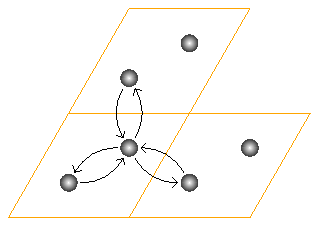
\includegraphics[width=0.48\textwidth]{Abbildungen/Raumstrukturen/Graphen.pdf}
		\caption{Mögliche $t$-Übergänge in Graphen bzgl. einer Elementarzelle}
		\label{Uebergaenge Graphen}
	\end{figure}
	%
	\begin{align}
		\vec H = \mat{\eC & z \\ \overline z & \eC} \quad \text{mit} \quad z = -t \bracks{1 + \E^{\I \vec t_1 \cdot \vec k} + \E^{\I \vec t_2 \cdot \vec k}}
		\label{Energiematrix Graphen}
	\end{align}
	%
	formulieren. Wie es sich hier schon andeutet, wird es auch später bei der Arbeit mit dem Tight-Binding-Modell im reziproken Raum immer auf die Diagonalisierung einer Matrix hinauslaufen, in der die Kopplungsenergien aller möglichen Übergänge -- auch in sich selbst, siehe Diagonale -- bzgl. der Zustände einer Elementarzelle aufgetragen sind. Spalten \emph{("`von"')} und Zeilen \emph{("`nach"')} sind letzteren in einheitlicher Reihenfolge zugeordnet. Wenn ein Übergang die Grenze der Elementarzelle überschreitet, wird der entsprechende Energieparameter mit einem Phasenfaktor, dem Eigenwert des zuständigen Translationsoperators, versehen.
	
	Hier erhält man die Energieeigenwerte etwa als Lösung von $\det(\vec H - E \vec 1) = 0$, wobei $\vec 1$ die Einheitsmatrix ist. Sie lauten
	%
	\begin{align*}
		E_\pm(\vec k) = \eC \pm |z| = \eC \mp t \sqrt{3 + 2 \cos(\vec t_1 \cdot \vec k) + 2 \cos(\vec t_2 \cdot \vec k) + 2 \cos((\vec t_2 - \vec t_1) \cdot \vec k)},
	\end{align*}
	%
    wobei $E_-$ das Valenz- und $E_+$ das Leitungsband beschreibt. Der Einfachheit halber kann man $\vec k$ statt durch $(k_x \ k_y)$ auch in Einheiten der reziproken Basisvektoren $\vec u_{1, 2}$ multipliziert mit $2 \pi$ angeben. Diese schiefwinkligen Koordinaten $(k_1 \ k_2)$ sind gerade durch die Skalarprodukte mit den Translationsvektoren gegeben, denn es gilt
	%
	\begin{align}
		k_n = \vec t_n \cdot \vec k = \vec t_n \cdot (c_1 \vec u_1 + c_2 \vec u_2) \overset{\rm Gl.~\ref{orthogonale tl}} = 2 \pi c_n \quad \text{für} \quad n \in \braces{1, 2}
		\label{Koordinaten}
	\end{align}
	%
	mit entsprechenden Linearkoeffizienten $c_n$. Damit ergibt sich schließlich
	%
	\begin{align}
		E_\pm(k_1, k_2) = \eC \pm t \sqrt{3 + 2 \cos(k_1) + 2 \cos(k_2) + 2 \cos(k_2 - k_1)}.
		\label{Eigenenergien Graphen}
	\end{align}
	%
	Um eine zweidimensionale aussagekräftige Darstellung zu ermöglichen, stellt man die Bandstruktur oft entlang ausgewählter Pfade durch eine reziproke Elementarzelle -- hier und für gewöhnlich die erste \textsc{Brillouin}-Zone -- dar, die die charakteristischsten Punkte linear verbinden.
	%
	Im Fall von Graphen sind letztere der $\vec \varGamma$-Punkt im Ursprung, an dem die Energie betragsmäßig am größten ist, $\vec K$ und $\vec K'$ -- nicht zu verwechseln mit den reziproken Gittervektoren -- an den beiden Schnittpunkten der Bänder auf \textsc{Fermi}-Niveau, und $\vec M$ auf halber Strecke zwischen $\vec K$ und $\vec K'$.\footnote{Diese \emph{"`special points"'} werden in \cite[S.~6]{Katsnelson1} definiert.} Eine mögliche Wahl ist
	%
	\begin{figure}
		\begin{minipage}[t]{0.48\textwidth}
			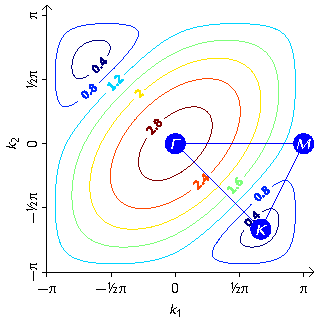
\includegraphics[width=\textwidth]{Abbildungen/Bandstrukturen/BZ_C2_1.pdf}
			\subcaption{Konturdarstellung des Leitungsbands mit Symmetriepfad in angepassten Koordinaten}
		\end{minipage}
		\hfill
		\begin{minipage}[t]{0.48\textwidth}
			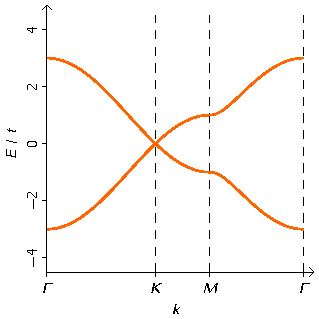
\includegraphics[width=\textwidth]{Abbildungen/Bandstrukturen/C2.pdf}
			\subcaption{Bandstruktur entlang ausgewähltem Pfad. Das Verhältnis der Abstände ist gewahrt.}
		\end{minipage}
		\caption{Dispersionsrelation von Graphen}
		\label{C2}
	\end{figure}
	%
	\begin{align*}
		\vec \varGamma = \mat{0 \\ 0}, \quad \vec K = \frac {\vec u_1 - \vec u_2} 3 = \frac{2 \pi}{3 \sqrt 3 a} \mat{1 \\ -\sqrt 3} \quad \text{und} \quad \vec M = \frac {\vec u_1} 2 = \frac \pi {3 a} \mat{\sqrt 3 \\ -1}.
	\end{align*}
	%
	Die Bandstruktur im Höhenprofil sowie entlang des Pfads $\vec \varGamma \rightarrow \vec K \rightarrow \vec M \rightarrow \vec \varGamma$ ist in Abb.~\ref{C2} dargestellt. Gut erkennbar sind die in der Einleitung erwähnte lineare Dispersion samt Schnittpunkt auf \textsc{Fermi}-Niveau bei $\vec K$ sowie das Plateau im Bereich von $\vec M$. Durch Vergleich mit Abb.~\ref{DOS Graphen} folgt, dass ersterer für das Minimum bei $E = 0$ und letzteres für die Maxima bei $E = \pm t$ in der Zustandsdichte verantwortlich ist, die in Kap.~\ref{Zustandsdichte} erläutert wird.
	
	\subsection{Beschreibung der Adsorbate}
	
	Es soll sich nun maximal ein Fremdatom bei jedem Kohlenstoffatom befinden können. Die genaue Geometrie der Bindung sei dabei nicht weiter bestimmt. Im verwendeten Modell sind jetzt lediglich weitere Elektronenübergänge zwischen Fremd- und jeweiligen Kohlenstoffatomen zugelassen. Mit den adsorbatabhängigen \emph{on-site}- und \emph{hopping}-Energien $\eX$ und $V$ muss der \textsc{Hamilton}-Operator dazu additiv um die Terme
	%
	\begin{align*}
		\op H_\text{X} = \eX \sum_{\vec R_\text{X}} \ket{\vec R_\text{X}} \ket{\rm X} \bra{\rm X} \bra{\vec R_\text{X}} \quad \text{und} \quad \op H_V = V \sum_{\vec R_\text{X}} \ket{\vec R_\text{X}} \ket{\rm C} \bra{\rm X} \bra{\vec R_\text{X}} + \text{h.c.}
	\end{align*}
	%
	ergänzt werden, wobei die Summe über alle $\nX$ Atompositionen $\vec R_\text{X}$ geht, an denen sich ein Fremdatom befindet.\footnote{Auch diese Beschreibung stammt sinngemäß aus \cite[S.~2]{Wehling2}, ist dort aber in zweiter Quantisierung formuliert.} $\ket{\vec R_\text{X}}$ ist dabei als Zustand bekannter Form $\ket{\vec R} \ket a$ bzw. $\ket{\vec R} \ket b$ anzusehen, während $\ket{\rm C}$ und $\ket{\rm X}$ einen weiteren Freiheitsgrad zur Unterscheidung zwischen Kohlenstoff- und Fremdatom einführen. X steht hier wie auch weiterhin stellvertretend für Wasserstoff H bzw. Fluor F. In dieser erweiterten Basis lässt sich $\eC$ natürlich nicht mehr einfach zu jedem Eigenwert hinzuaddieren. Der \textsc{Hamilton}-Operator in Gl.~\ref{Hamiltonian Graphen} gilt nur auf dem zu $\ket{\rm C}$ gehörigen Unterraum.
	
	Genügt eine Adsorbatstruktur ebenfalls einer einfachen Periodizität, bietet es sich an im reziproken Raum zu arbeiten und explizite Energiebänder zu berechnen. Ist die Translationssymmetrie gebrochen, ist es hingegen sinnvoll in den Ortsraum überzugehen.
	
	\subsection{Arbeit im Ortsraum}
	
	Die Eigenzustände eines endlichen Systems sind diskret: Für eine Superzelle aus $l \times l$ Elementarzellen sind wegen der periodischen Randbedingungen auch nur noch $l^2$ $\vec k$-Werte innerhalb einer reziproken Elementarzelle erlaubt, bei entsprechender Wahl letzterer etwa
	%
	\begin{align*}
		k_{1, 2} = 2 \pi \frac n l \quad \text{mit} \quad n \in { 0, 1 \dots l - 1 }
	\end{align*}
	%
	Wenn man nicht am genauen Verlauf der Bänder sondern nur an den Energieeigenwerten interessiert ist, sollte man den reziproken Raum verlassen und im Ortsraum arbeiten.
	
	Die Größe -- also Zeilen- bzw. Spaltenanzahl -- der zu diagonalisierenden Matrix kann dann nicht mehr über \textsc{Fourier}-Analysis auf die Anzahl der Zustände innerhalb einer Elementarzelle reduziert werden, sondern ist immer gleich der Gesamtzahl von Zuständen im System, d.h. hier der Anzahl von Atomen in der Superzelle. Dafür sind die nicht verschwindenden Matrixelemente nun ausschließlich durch die Energieparameter ohne komplexe Phasenfaktoren gegeben. Elektronen-\emph{hopping} aus der Superzelle hinaus führt per Definition einfach an den gegenüberliegenden Rand.\footnote{Es ist natürlich auch hier möglich Phasenfaktoren verwenden, die Superzelle also als neue Elementarzelle zu betrachten. Die Anzahl der Bänder ist dann entsprechend hoch.}
	
	Im Falle reinen Graphens bedeutet das, dass zur Berechnung aller Eigenenergien -- von der Möglichkeit Gl.~\ref{Eigenenergien Graphen} zu verwenden abgesehen -- an Stelle von $l^2$ $2 \times 2$-Matrizen eine Matrix der Größe $\nC = 2 l^2$ diagonalisiert werden muss.
	
	Um jedem der $\nC$ Kohlenstoffatome eindeutig eine Zeile bzw. Spalte der Energiematrix zuordnen zu können, werden die entsprechenden $(i \ j \ k)$ zu einem Index
	%
	\begin{align*}
		N = 2 (i l + j) + k
	\end{align*}
	%
	zusammengefasst, der eine Sortierung nach $i$, $j$ und $k$ in absteigender Rangfolge vornimmt. Ausgehend vom größten $N = 2 ((l - 1) l + l - 1) + 1 = 2 l^2 - 1 = \nC - 1$ der Kohlenstoffatome werden die $\nX$ Adsorbate einfach weiter durchnummeriert und erhalten so die Indizes
	%
	\begin{figure}
		\begin{minipage}[b]{0.48\textwidth}
			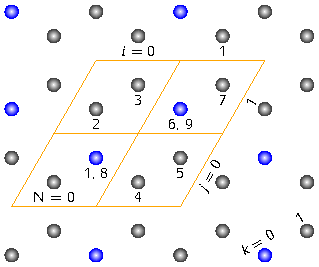
\includegraphics[width=\textwidth]{Abbildungen/Raumstrukturen/Ortsraumbeispiel.pdf}
			\subcaption{Superzelle der Größe $l = 2$: Bei Angabe zweier Indizes bezieht sich ersterer auf das Kohlenstoff- und letzterer auf das Fremdatom.}
			\label{Ortsraumbeispiel}
		\end{minipage}
		\hfill
		\begin{minipage}[b]{0.48\textwidth}
			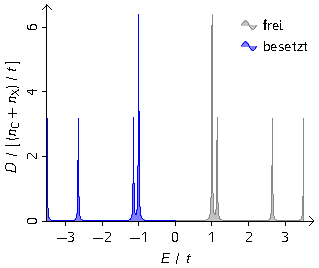
\includegraphics[width=\textwidth]{Abbildungen/Zustandsdichten/Ortsraumbeispiel.pdf}
			\subcaption{Zustandsdichte im undotierten Fall: Hier wird jeder diskrete Eigenwert durch eine \textsc{Lorentz}-Kurve der Halbwertsbreite $t / 100$ dargestellt.}
			\label{Ortsraumbeispiel DOS}
		\end{minipage}
		\caption{Beispielsystem für Arbeit im Ortsraum}
	\end{figure}
	%
	\begin{align*}
		N = \nC + n \quad \text{mit} \quad n \in \braces{0 \dots n_\text{X} - 1}.
	\end{align*}
	%
	Beispielhaft wird hier das in Abb.~\ref{Ortsraumbeispiel} gezeigte System aus acht Kohlenstoff- und zwei Fremdatomen behandelt. Die Energien aller möglichen Übergänge sind in der Matrix
	%
	\begin{align*}
		\vec H = \bordermatrix{
		    \color{grey} N & \color{grey} 0 & \color{grey} 1 & \color{grey} 2 & \color{grey} 3 & \color{grey} 4 & \color{grey} 5 & \color{grey} 6 & \color{grey} 7 & \color{grey} 8 & \color{grey} 9 \cr
			\color{grey} 0 & \eC & t   & 0   & t   & 0   & t   & 0   & 0   & 0   & 0 \cr
			\color{grey} 1 & t   & \eC & t   & 0   & t   & 0   & 0   & 0   & V   & 0 \cr
			\color{grey} 2 & 0   & t   & \eC & t   & 0   & 0   & 0   & t   & 0   & 0 \cr
			\color{grey} 3 & t   & 0   & t   & \eC & 0   & 0   & t   & 0   & 0   & 0 \cr
			\color{grey} 4 & 0   & t   & 0   & 0   & \eC & t   & 0   & t   & 0   & 0 \cr
			\color{grey} 5 & t   & 0   & 0   & 0   & t   & \eC & t   & 0   & 0   & 0 \cr
			\color{grey} 6 & 0   & 0   & 0   & t   & 0   & t   & \eC & t   & 0   & V \cr
			\color{grey} 7 & 0   & 0   & t   & 0   & t   & 0   & t   & \eC & 0   & 0 \cr
			\color{grey} 8 & 0   & V   & 0   & 0   & 0   & 0   & 0   & 0   & \eX & 0 \cr
			\color{grey} 9 & 0   & 0   & 0   & 0   & 0   & 0   & V   & 0   & 0   & \eX }
	\end{align*}
	%
	aufgeführt. Sie liefert neun Energieeigenwerte. Das Spektrum ist für $\eX = 0$ in Abb.~\ref{Ortsraumbeispiel DOS} grafisch dargestellt.
	
	\subsection[Elektronische Zustandsdichten und die \textsc{Fermi}-Verteilung]{Elektronische Zustandsdichten und die \textsc{Fermi}-Verteilung\footnote{Auch hier lässt sich der allgemeingültige Teil der Information in \cite[S.~132f]{Czycholl} wiederfinden.}}
	\label{Zustandsdichte}
	
	\begin{figure}
		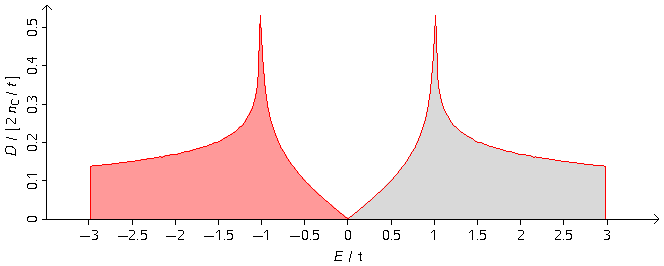
\includegraphics[width=\textwidth]{Abbildungen/Bandstrukturen/DOS_C2.pdf}
		\caption[Zustandsdichte von Graphen]{Zustandsdichte von Graphen, berechnet als Histogramm. Genauer wurden hier $600 \times 600$ Energieeigenwerte 201 aufeinanderfolgenden Energieintervallen konstanter Breite zugeordnet. Die Zahl letzterer ist ungerade, damit der charakteristische Punkt für $E = 0$ nicht auf eine Intervallgrenze fällt. Dieser wird, wie jeder Knick in einer Zustandsdichte als \emph{\textsc{van-Hove}-Singularität} \cite{vanHove} bezeichnet.}
		\label{DOS Graphen}
	\end{figure}
	%
	Es wurde nun bereits zweimal von der elektronischen Zustandsdichte $D(E)$ Gebrauch gemacht. Ihre Definition für diskrete Eigenzustände $E_i$ mit $i \in \braces{1 \dots n}$ und $E_i \leq E_j$ für $i < j$ lautet
	%
	\begin{align*}
		D(E) = \sum_{i = 1}^n \delta(E - E_i), \quad \text{so dass} \quad \nE = \int_{\mathrlap{-\infty}}^{\mathrlap{E_\mathrm{F}}} \D E \, D(E)
	\end{align*}
	%
	im Grundzustand, also für $T = 0$, die Anzahl der besetzten Zustände bis zum \textsc{Fermi}-Niveau $E_\mathrm{F}$, d.h. die Anzahl der Elektronen im System ist. Dessen Gesamtenergie -- die später zu minimierende Größe -- ist dann einfach die Summe der $\nE$ kleinsten Energieeigenwerte, also
	%
	\begin{align*}
		E_\Sigma = \int_{\mathrlap{-\infty}}^{\mathrlap{E_\mathrm{F}}} \D E \, D(E) E = \sum_{i = 1}^{\nE} E_i.\footnotemark
	\end{align*}
	%
	Sie wird nur nur hier als $E_\Sigma$ bezeichnet. Im weiteren Verlauf der Arbeit wird die Variable $E$ kontextabhängig für verschiedene Energien verwendet.
	
	Die $\delta$-Distribution hat stets die reziproke Einheit ihres Arguments. Dasselbe gilt folglich für $D$ und die Größe auf die sie sich bezieht, hier die Energie. Da sich $\delta(E)$ nicht exakt grafisch darstellen lässt, muss beispielweise auf eine \textsc{Lorentz}-Kurve ausgewichen werden.
	
	Während der Spin $\nicefrac 1 2$ des Elektrons bislang vernachlässigt wurde, soll er von nun an berücksichtigt werden, allerdings nur in der Hinsicht, dass alle Energieeigenwerte durch ihn zweifach entartet sind, das Auftreten jedes Eigenwerts also verdoppelt wird.\footnotetext{Der Vollständigkeit halber sei angemerkt, dass diese Formel nur gilt, weil die \\ \textsc{Fermi}-Verteilung $f(E) = \parens{1 + \exp \frac{E - \mu}{k T}}^{-1}$ für $T \rightarrow 0$ in die \textsc{Heaviside}-Funktion $\Theta(E - \mu) = \begin{cases} 1 & E \geq \mu \\ 0 & E < \mu \end{cases}$ übergeht, \\ wobei das \emph{chemische Potential} $\mu = E_\mathrm{F}$ für $T = 0$. Ansonsten müsste man $E_\Sigma = \int \limits_{-\infty}^\infty \D E \, \rho(E) f(E) E$ schreiben.}
	
	Ohne Ladungsdotierung trägt jedes beteiligte Atom -- sowohl C als auch X -- ein $\pi$-Elektron bei. Wegen der Spinentartung gibt es also genau doppelt so viel Zustände wie Elektronen, was für reines Graphen bedeutet, dass das Valenzband vollständig besetzt, das Leitungsband hingegen leer ist (siehe Abb.~\ref{DOS Graphen}). Abweichende Ladungsträgerzahlen $\nE$ werden hier durch die auf $\nC$ bezogene Konzentration $\cE$ zusätzlicher Elektronen ausgedrückt, also
	%
	\begin{align*}
		\nE = (1 + \cE) \nC + \nX, \quad \text{wobei} \quad \nX = \cX \nC
	\end{align*}
	%
	selbst durch eine entsprechende Adsorbatkonzentration $\cX$ angegeben wird.
	
	\section{Wandel der Adsorbatstruktur}
	
	\subsection[Das kanonische Ensemble]{Das kanonische Ensemble\footnote{Herleitung angelehnt an \cite[S.~113, 119]{Nolting}}}
	
	Um günstige Adsorbatkonfigurationen zu finden, muss man zulassen, dass die Fremdatome ihre Positionen ändern können. Dabei sei es hier nicht von Belang, ob dieser Vorgang im realen physikalischen System auch so ablaufen würde.
	
	Zu statistischen Aussagen gelangt man dann einerseits über zeitliche Mittelwertbildung. Wenn die Bewegung es zulässt, dass auf Dauer jede theoretisch mögliche Konfiguration erreicht werden kann, gibt es zudem die Möglichkeit über ein \emph{Ensemble} statischer Systeme zu mitteln, das jeden dieser \emph{Mikrozustände} $\ket{\psi_i}$ mit einer bestimmten Gewichtung $p_i$ beinhaltet. Beide Ansätze führen in einem sogenannten \emph{ergodischen} System zu gleichen makroskopischen Ergebnissen.\footnote{\emph{"`Um die genannten Zeitmittel zu berechnen, geht \emph{Boltzmann} \emph{[Gastheorie II, \S 34, 1898]} aus von der Fiktion einer Schaar von unendlich vielen gleichbeschaffenen Exemplaren des vorgegebenen Gasmodells, \emph{[\dots]}"'}, fassen \textsc{Paul und Tatjana Ehrenfest} zusammen bevor sie die postulierte Gleichheit von "`Zahlmittel"' und "`Zeitmittel"' diskutieren. \cite[S.~34]{Ehrenfest1}}
	
	In der Ensembleformulierung lautet der Erwartungswert einer Observablen $\op A$
	%
	\begin{align*}
		\av{\op A} &= \sum_i p_i \bra{\psi_i} \op A \ket{\psi_i} = \sum_{i, m, n} p_i \bracket {\psi_i} m \bra m \op A \ket n \bracket n {\psi_i} \\
		&= \sum_{i, m, n} p_i \bra m \op A \ket n \bracket n {\psi_i} \bracket {\psi_i} m = \sum_{i, m} p_i \bra m \op A \ket{\psi_i} \bracket {\psi_i} m = \operatorname{tr}(\op A \op \rho)
	\end{align*}
	%
	mit beliebigen Orthonormalbasen $\braces{\ket m}$ und $\braces{\ket n}$ sowie dem \emph{statistischen Operator}
	%
	\begin{align}
		\op \rho = \sum_i p_i \ket{\psi_i} \bra{\psi_i}.\footnotemark
		\label{statistischer Operator}
	\end{align}
	%
	Man bildet also das makroskopische Mittel der mikroskopischen quantenmechanischen Erwartungswerte -- die $\ket{\psi_i}$ können durchaus Superpositionen beschreiben --, womit zwei grundsätzlich verschiedene Arten der Unsicherheit involviert sind.\footnotetext{zu finden im Kap. 33 "`The Gibbs ensemble"' in \textsc{Diracs} Lehrbuch \cite[S.~132]{Dirac}}
	
	Da sich mit der Adsorbatstruktur im Allgemeinen auch die Gesamtenergie verändert, kann das System auf Grund der Energieerhaltung nicht isoliert sein. Vielmehr handle es sich um ein Teilsystem $\Sigma_1$ in Kontakt mit einem Wärmebad $\Sigma_2$, das die Gesamtenergie $E$ und eine globale Temperatur $T$ konstant hält.\footnote{Da die Temperatur, die hier die Bewegung der Adsorbate erlaubt, virtueller Natur sei, habe sie keinerlei Einfluss auf die Elektronenkonfiguration, die stets im Grundzustand bei $T = 0$ verharre.} $\Sigma_1$ wird durch ein sogenanntes \emph{kanonisches}, das isolierte Gesamtsystem $\Sigma = \Sigma_1 \cup \Sigma_2$ mit der konstanten Gesamtenergie $E$ hingegen durch ein \emph{mikrokanonisches Ensemble} beschrieben.
	
	Seien die $\ket{\psi_i}$ nun Eigenzustände in $\Sigma_1$ zu den Energien $E_i$. Ohne weitere Annahmen muss man jedem Mikrozustand des Gesamtsystems, der mit einer gegebenen Verteilung der Energie verträglich ist, die gleiche Wahrscheinlichkeit zusprechen. Umgekehrt ist die Wahrscheinlichkeit $P(E_i)$ für $E_i$ in $\Sigma_1$ proportional zur Anzahl $\mathit \Gamma(E_i) = \mathit \Gamma_1(E_i) \mathit \Gamma_2(E - E_i)$ ebendieser Zustände, wobei die \emph{Phasenvolumina} $\mathit \Gamma_1$ und $\mathit \Gamma_2$ angeben, auf wie viele Arten sich die Energie im Argument im entsprechenden System im Rahmen einer kleinen Toleranz realisieren lässt.
	
	Falls es $\Gamma_1(E_i) > 1$ verschiedene $i$ mit gleichen $E_i$ gibt, gilt das gerade eingeführte \emph{Prinzip der gleichen a-priori-Wahrscheinlichkeit}\footnote{\emph{"`For the development of statistical mechanics it has been found necessary to introduce a pair of assumptions, which may be designated together as the hyopthesis of \emph{equal} a priori \emph{probabilities and of random} a priori \emph{phases} for the quantum states of a mechanical system."'} \cite[S.~4]{Tolman}} gleichermaßen für die betreffenden $\ket{\psi_i}$. Es folgt
	%
	\begin{align}
		p_i = \frac{P(E_i)}{\mathit \Gamma_1(E_i)} \propto \Gamma_2(E - E_i).
		\label{Systemwahrscheinlichkeit}
	\end{align}
	%
	Für die Änderung der Entropie $S$ mit der inneren Energie $E$ findet man allgemein
	%
	\begin{align*}
		\pdiff S E = \frac 1 T \quad \text{und damit} \quad \Delta S = \frac {\Delta E} T \quad \text{für} \quad T = \text{const.}
	\end{align*}
	%
	Für die statistische Entropie $S_2(E)$ in $\Sigma_2$ gilt daher
	%
	\begin{align*}
		S_2(E - E_i) = S_2(E) - \frac {E_i} T \quad \text{bzw.} \quad \Gamma_2(E - E_i) = \Gamma_2(E) \cdot \E^{-\frac{E_i}{k T}}
	\end{align*}
	%
	nach Einsetzen ihrer Definition $S_2(E) = k \log \Gamma_2(E)$ mit der \textsc{Boltzmann}-Konstanten $k$. Über Gl.~\ref{statistischer Operator} und \ref{Systemwahrscheinlichkeit} liefert dieses Ergebnis als statistischen Operator des kanonischen Ensembles
	%
	\begin{align*}
		\op \rho = \frac 1 Z \sum_i \ket{\psi_i} \E^{-\frac{E_i}{k T}} \bra{\psi_i} = \frac 1 Z \sum_i \E^{-\frac{\op H}{k T}}, \quad \text{wobei} \quad Z = \operatorname{tr} \E^{\frac{\op H}{k T}}
	\end{align*}
	%
	die \emph{kanonische Zustandssumme} und $\op H$ der \textsc{Hamilton}-Operator für $\Sigma_1$ ist. Das Maximum dieser Verteilung liegt trotz des exponentiellen Zusammenhangs im Allgemeinen oberhalb der kleinsten Energie, was durch $\mathit \Gamma_1(E_i)$, bzw. dadurch zu erklären ist, dass jede Eigenenergie $E_i$ zusätzlich mit ihrem Entartungsgrad $g_i$ gewichtet ist (siehe Abb.~\ref{Phasenvolumen}).
	
	\subsection[Der \textsc{Metropolis}-Algorithmus]{Der \textsc{Metropolis}-Algorithmus\footnote{1953 motiviert und beschrieben von \textsc{Metropolis}, \textsc{Rosenbluth}, \textsc{Rosenbluth}, \textsc{Teller} und \textsc{Teller} \cite{Metropolis2}}}
	
	Hat man es wie hier mit so großen Ensembles zu tun, dass es im Rahmen der verfügbaren Rechenleistung unmöglich ist, alle möglichen Mikrozustände in numerische Berechnungen mit einzubeziehen -- es gibt $\nC! \, / \, \bracks{\nX! \ (\nC - \nX)!}$ verschiedene Konfigurationen, wobei ein Großteil symmetrisch äquivalent ist --, dann bietet es sich an, auf eine \emph{Monte-Carlo-Methode} zurückzugreifen, sich also auf eine repräsentative Teilmenge des Ensembles zu beschränken, deren Wahl in irgendeiner Weise vom Zufall abhängt.\footnote{\emph{"`It is obviously impossible to count all of them. Here again the more sensible approach would be to take, say $10^4$ points at random from this ensemble and examine those only; \emph{[\dots]}. It follows from simple application of ergodic theorems that the estimate should be, with great probability, valid within a few per cent."'} \cite[S.~336f]{Metropolis1}}
	
	Im Fall des kanonisches Ensembles der Adsorbatkonfigurationen könnte man beispielsweise so lange zufällig Summanden des statistischen Operators streichen, bis die gewünschte Größe erreicht ist. Das Problem, dass viele Summanden mit einem verhältnismäßig verschwindend kleinen Gewicht $\exp(-E_i / k T)$ prozessiert werden, die entsprechend nur einen kleinen Beitrag zu etwaigen Mittelwerten liefern, ist dadurch aber noch nicht gelöst.
	
	Die Idee hinter dem \textsc{Metropolis}-Algorithmus ist deshalb die Erzeugung eines Ensembles konstanter Gewichtung, das sich in Bezug auf Erwartungswerte nicht vom Originalensemble unterscheiden soll. Dazu werden Mikrozustände aus letzterem nur noch mit einer gewissen Wahrscheinlichkeit entsprechend ihrer ursprünglichen Gewichtung übernommen.\footnote{\emph{"`\emph{[\dots]} instead of choosing configurations randomly, then weighting them with $exp(-E / k T)$, we choose configurations with a propability $exp(-E / k T)$ and weight them evenly."'} \cite[S.~1088]{Metropolis2}} 
	
	Konkret wird, beginnend mit einem beliebigem Ausgangszustand der Energie $E_0$, durch wiederholte Ausführung folgender Schritte eine sogenannte \textsc{Markov}-Kette erster Ordnung erzeugt,\footnote{Gedächtnisloser Zufallsprozess: erzeugt eine Folge, dessen jeweils nächstes Glied nur vom aktuellen abhängen darf. In der namensgebenden Veröffentlichung \cite{Markov} analysiert \textsc{Markov} den Roman \emph{Eugene Onegin} von \textsc{Puschkin} in Bezug auf Zeichenfolgen. So  ermittelt er Wahrscheinlichkeiten dafür, dass Ausdrücke bestimmter Typen im Text aufeinander folgen. Mit vergleichbarem Wissen kann man beispielsweise Daten auf untypische Sequenzen untersuchen.} deren Glieder der kanonischen bzw. \textsc{Boltzmann}-Verteilung genügen:
	%
	\begin{enumerate}
		\item Erzeuge eine geringfügige, zufällige Variation des letzten Zustands der Kette.
		\item Berechne deren Energie $E$.
		\item Ist $\exp \parens{\frac{E_0 - E}{k T}}$ größer als eine gleichverteilte Zufallszahl zwischen 0 und 1?
		\begin{itemize}
			\item[\emph{Ja:}] Erweitere die Kette um neuen Zustand und setzte $E_0 = E$.
			\item[\emph{Nein:}] Füge den alten Zustand erneut hinzu.
		\end{itemize}
	\end{enumerate}
	%
	Durch konsekutive Anwendung der Variation muss jeder Zustand des Ensembles erreichbar sein, so dass die Ergodizität gewährleistet ist. Die Adsorbatbewegung wird hier so realisiert, dass einem einzelnen Fremdatom bei $(x_0 \ y_0)$ über die gleichverteilten Zufallszahlen
	%
	\begin{align*}
		r \in [0, R] \quad \text{und} \quad \phi \in [0, 2 \pi]
	\end{align*}
	%
	innerhalb eines Radius $R$ ein neuer Ort zugewiesen wird mit
	%
	\begin{align*}
		x = x_0 + r \cos(\phi) \quad \text{und} \quad y = y_0 + r \sin(\phi).
	\end{align*}
	%
	Dieser wird dann über Gl.~\ref{ijk} auf eine Kohlenstoffposition "`gerundet"'. Wenn sich dort schon ein Fremdatom befindet, wird der Schritt nicht vollzogen. Im nächsten Schleifendurchlauf wird dann versucht ein anderes Fremdatom zu bewegen. Erst wenn alle einmal prozessiert wurden, darf erneut mit dem ersten begonnen werden.
	
	\subsection[Simulated Annealing]{Simulated Annealing\footnote{Diese Methode wurde laut \cite[Einleitung]{vanLaarhoven} erstmals 1883 in einer Veröffentlichung von \textsc{Kirkpatrik} et al. \cite{Kirkpatrick} vorgeschlagen, an der sich dieser Abschnitt orientiert.}}
	
	Letztendlich gilt das Interesse hier nicht einem Ensemble und resultierenden Mittelwerten, sondern einer einzelnen Konfiguration, die sich nicht mehr verändert. Dazu muss der Grenzfall $T \rightarrow 0$ betrachtet werden, in dem die \textsc{Boltzmann}-Faktoren $\exp(-E / k T)$ mit zunehmender Energie unendlich schnell abfallen. Unabhängig von Vielfachheiten höherer Energieeigenwerte wird das System deshalb in einen Grundzustand streben.\footnote{\emph{"`\emph{[\dots]} as $T$ is lowered the Boltzmann distribution collapses into the lowest energy state or states."' \cite[S.~672]{Kirkpatrick}}}
	
	In Analogie zur Bereinigung eines Kristalls von Fehlordnungen durch Ausglühen (engl. \emph{"`anneal"'}), d.h. Schmelzen gefolgt von kontrolliertem und besonders im Bereich des Gefrierpunkts langsamem Abkühlen,\footnote{\emph{"`If this is not done, and the substance is allowed to get out of equilibrium, the resulting crystal will have many defects \emph{[\dots]}."' \cite[S.~672]{Kirkpatrick}}} wird beim \emph{Simulated Annealing} das Abkühlen eines Modellsystems mit Hilfe des Computers nachgeahmt. Einen entsprechenden Algorithmus erhält man, indem man den \textsc{Metropolis}-Algorithmus um einen weiteren Schritt ergänzt:
	%
	\begin{enumerate}
	    \setcounter{enumi}{3}
		\item Multipliziere $T$ mit einem Faktor $f \in (0, 1)$.
	\end{enumerate}
	%
	In Anlehnung an das Abkühlungsgesetz von \textsc{Newton} wird das System auf diese Weise exponentiell, also mit abnehmendem Abstand vom absoluten Nullpunkt immer langsamer abgekühlt. Es kann sinnvoll sein diesen Schritt nach jeder Durchführung für einige Schleifendurchläufe auszusetzen, damit das System wieder ins Gleichgewicht findet.\footnote{So erhält man die im Originalpaper verwendete Kühlung \cite[S.~675]{Kirkpatrick}. Je nach Problemstellung lassen sich oft effizientere Vorschriften finden \cite[S.~59f]{vanLaarhoven}.}
	
	In Verbindung mit der Wahl einer geeigneten Ausgangstemperatur $T$ hofft man das System nun in den Grundzustand bzw. allgemein in ein globales Extremum der zu optimierenden Größe oder \emph{Zielfunktion} zu bewegen, indem die anfängliche Freiheit auch Energieerhöhungen in Kauf zu nehmen das "`Hängenbleiben"' in lokalen Extrema verhindert.
	
	Weil die Temperatur hier nur ein Maß für die Bereitwilligkeit eines Zustands ist, einen energetisch ungünstigen Übergang zu vollziehen, kann im Modell $k = 1$ gesetzt und $T$ als Energieparameter betrachtet werden.
	
	\subsection{Hill Climbing}
	\label{Hill Climbing}
	
	Da es beim Kühlen auf eine gewisse Langsamkeit ankommt, kann Simulated Annealing mit einem sehr hohen Rechenaufwand verbunden sein, besonders wenn die bei jeder Iteration nötige Berechnung der Zielfunktion kostspielig ist.\footnote{siehe auch \cite[S.~139]{vanLaarhoven}} In solchen Fällen kann ein \emph{Hill-Climbing}-, also \emph{"`Bergsteiger"'-Algorithmus} die bessere Alternative sein.
	
	Es handelt sich dabei um einen Spezialfall von Simulated Annealing, bei dem von vornherein die "`Temperatur"' $T = 0$ gesetzt wird, also nur Schritte zugelassen sind, die die Zielfunktion unmittelbar optimieren.\footnote{\emph{"`In hill-climbing search, we select any local change that improves the current value of the objective function."'} \cite[S.~334]{Selman}} Auf diese Weise werden häufig schnelle Fortschritte verzeichnet, unter Inkaufnahme der Einschränkung, dass ein erreichtes lokales Extremum\footnote{Das bedeutet hier, dass keine der möglichen Variationen der momentanen Konfiguration die Energie verringert.} endgültig ist. Dieses Problem kann etwa durch wiederholte Durchführung kompensiert werden.\footnote{\emph{"`\emph{[\dots]}, it is customary to carry out the process several times, starting from different randomly generated configurations, and save the best result."'} \cite[S.~672]{Kirkpatrick}}
    
	\section{Phasenübergänge}
	
	Der Begriff \emph{"`Phase"'} leitet sich vom altgriechischen "`$\phi \acute \alpha \sigma \iota \varsigma$"' ab und bedeutet so viel wie "`Erscheinung"'.\footnote{Übersetzung aus \cite[S.~778]{Schmidt}} In der Physik wird der Begriff in verschiedenen Zusammenhängen verwendet, oft in Bezug auf einen Zustand im weitesten Sinne, vgl. den "`Phasenraum"' oder die "`Phase"' einer Schwingung. Speziell in der Thermodynamik steht er allerdings für jeden "`homogenen Teil eines Systems"',\footnote{laut DIN 1345:1993-12 [\url{http://www.din-term.din.de/}, 21. August 2014] zu Grundbegriffen der Thermodynamik} also einen von bestimmten Zustandsgrößen aufgespannten Bereich, in dem eine betrachtete abhängige Größe sich nicht verändert. Die Existenz mehrerer Phasen bedingt folglich irgendeine Form von \emph{Phasenübergängen}, die es zu klassifizieren gilt.
	
	Das diesbezüglich wohl bekannteste Beispiel ist das Phasendiagramm von Wasser, dass dessen Aggregatzustände "`fest"', "`flüssig"' oder "`gasförmig"' -- vom überkritischen Fluid sei einmal abgesehen -- in Abhängigkeit von Druck $p$ und Temperatur $T$ darstellt. Auch innerhalb einer Phase können zwar Veränderungen anderer Größen stattfinden -- etwa des Volumens im Falle eines Gases --, die Zuordbarkeit der Aggregatzustände ist dadurch aber nicht gestört. Eine Ausnahme stellen die genannten Phasenübergänge dar, die als \emph{Koexistenzlinien} benachbarter Phasen in Erscheinung treten.
	
	\subsection{Klassifizierung nach \textsc{Ehrenfest}}
	
	Zunächst sei angemerkt, dass die hier betrachteten Phänomene sich immer auf den Gleichgewichtsfall beziehen. Ob es beim schnellen Überschreiten einer Phasengrenze in Wirklichkeit zu einer \emph{Hysterese}, also einer verzögerten Einstellung auf die neuen Gegebenheiten, kommen würde, sei außer Acht gelassen. Die Annahme ist also, dass das System in jedem Punkt bereits genug Zeit hatte, das Gleichgewicht zu erreichen.
	
	Thermodynamisch entspricht das der Minimierung des jeweiligen \emph{thermodynamischen Potentials} in Bezug auf die vorgegebenen \emph{natürlichen Variablen}. Für den genannten Fall, dass $p$ und $T$ (sowie die Teilchenzahl $N$, die hier aber als konstant betrachtet wird) gegeben sind, ist das das \emph{freie Enthalpie} oder \emph{\textsc{Gibbs}-Energie} $G$ mit dem totalen Differential
	%
	\begin{align*}
		\D G = V \D p - S \D T + \mu \D N,
	\end{align*}
	%
	wobei $V$ das Volumen, $S$ die Entropie und $\mu$ das chemische Potential ist. Man erhält sie, wie die anderen Potentiale auch, über eine geeignete \textsc{Legendre}-Transformation aus der \emph{Fundamentalgleichung} $\D E = T \D S - p \D V + \mu \D N$ mit der inneren Energie $E$.\footnote{siehe Kap. 6.2 \emph{"`Die thermodynamischen Potentiale"'} in \cite{Jelitto}}
	
	Da sich alle thermodynamisch relevanten Größen durch ein- bis mehrfache partielle Ableitungen aus $G$ herleiten lassen, muss sich auch ein Phasenübergang in ihr niederschlagen. Dieser Idee folgend, führte \textsc{Ehrenfest} im Jahr 1933 eine Klassifizierung ein, die jedem Phasenübergang eine Ordnung zuweist, die angibt in der wievielten Ableitung von $G$ nach einer natürlichen Variablen die erste Unstetigkeit auftritt:\footnote{einschließlich der folgenden Beispiele für Übergänge erster und zweiter Ordnung zu finden in \cite[S.~155]{Ehrenfest2}}
	%
	\begin{itemize}
		\item[] \emph{Phasenübergänge nullter Ordnung} kann es danach nicht geben, da sich in $G$ als Integral über die ersten partiellen Ableitungen deren Unstetigkeiten nur als Knicke zeigen.
		
		\item[] \emph{Phasenübergänge erster Ordnung} hingegen zeichnen sich durch eine Umwandlungswärme $Q$ und eine Volumenänderung $\Delta V$ aus, denn
		%
		\begin{align*}
			\Delta \bracks{\pdiff G T} = -\Delta S = -\frac Q T \quad \text{und} \quad \Delta \bracks{\pdiff G p} = \Delta V,
		\end{align*}
		%
		wobei die Differenzen $\Delta \dots$ jeweils zwischen den Werten unmittelbar nach und vor dem Übergang zu bilden sind. 
	
		\item[] \emph{Phasenübergänge zweiter Ordnung} schließlich können sich etwa in einem Sprung in der spezifischen Wärme $c$ zeigen:
		%
		\begin{align*}
			\Delta \bracks{\pdiff{^2G}{T^2}} = \Delta \bracks{\pdiff S T} = \Delta \bracks{\pdiff S E \pdiff E T} = \frac {\Delta c} T.
		\end{align*}
		%
		\item[] \emph{Phasenübergänge höherer Ordnungen} sind nach diesem Prinzip durchaus denkbar.
	\end{itemize}
	%
	Die \textsc{Ehrenfest}-Klassifizierung wurde heute weitestgehend von neueren Ansätzen abgelöst. Durchgesetzt hat sich allerdings die Einteilung in Ordnungen, wenn auch nur folgende zwei: \emph{Diskontinuierliche Phasenübergänge} oder solche erster Ordnung zeichnen sich durch eine Unstetigkeit im sogenannten \emph{Ordnungsparameter} aus, die bei den \emph{kontinuierlichen Phasenübergängen} zweiter Ordnung nicht vorkommt.\footnote{siehe \cite[S.~315]{Fliessbach}}
	
	\subsection{Ordnungsparameter}
	
	Ein grundlegendes Konzept im Zusammenhang mit Phasenübergängen wurde bisher nicht genannt: der Symmetriebruch. Ein einfaches Beispiel hierfür ist das Gefrieren einer Flüssigkeit unter Bildung eines Kristalls. Während die Flüssigkeit invariant gegenüber beliebigen Rotationen und Translationen ist -- wobei man sich natürlich keine Momentaufnahme einer Ansammlung klassischer Teilchen vorstellen darf --, ist die Menge der Transformationen, die das periodische Kristallgitter in sich selbst überführen, stark eingeschränkt.\footnote{anschaulich dargestellt in \cite[S.~2]{Sethna}}
	
	Nach \textsc{Ehrenfest} handelt sich um einen Phasenübergang erster Ordnung, da er mit einem Wärmeaustausch und einer Volumenänderung einhergeht. Er ist zudem diskontinuierlich in der Hinsicht, dass die Ordnung schlagartig einsetzt, die beiden beteiligten Phasen sich also strukturell in keinster Weise ähneln.
	
	Nun ist es aber auch möglich, dass die Ordnung sich in einem kontinuierlichen Prozess einstellt -- im Gegensatz zur Symmetrie, die durch das Auftreten kleinster Unregelmäßigkeiten schon rein mathematisch sofort gebrochen ist.\footnote{\emph{"`The configuration of atoms in the crystal changes continuously. However, an arbitrarily small displacement of the atoms from their original symmetrical position is sufficient to change the symmetry of the lattice."'} \cite[S.~447]{Landau2}} In diesem Zusammenhang führte \textsc{Landau} 1937 die Ordnungsparameter ein. Für gewöhnlich sind sie so definiert, dass sie im symmetrischen, ungeordneten System verschwinden und mit zunehmender Ordnung endliche Werte annehmen.\footnote{\emph{"`In the general theory of such \emph{[of the second kind]} transitions there always enters some \emph{[order]} parameter $\eta$ which differs from zero in the ordered phase and which equals zero in the disordered phase."'} \cite[S.~546]{Landau1}} Bei Phasenübergängen zweiter Ordnung ist dieser Verlauf wie bereits erwähnt stetig,\footnote{\emph{"`A passage through a phase transition point of the second kind has a continuous change of $\eta$ to zero."'} \cite[S.~450]{Landau2}} weshalb die Verbindung zu thermodynamischen Größen über die Entwicklung eines thermodynamisches Potentials im Bereich des Übergangs nach Potenzen des Ordnungsparameters hergestellt werden kann.\footnote{siehe \S~143 "`The discontinuity of specific heat"' in \cite[S.~451ff]{Landau2}}
	
	Ein Beispiel ist der Übergang zweiter Ordnung vom Para- zum Ferromagnetismus bei \emph{\textsc{Curie}-Temperatur}: Mit der zunehmend uniformen Ausrichtung der zuvor ungeordneten Spins wird mikroskopisch die Rotationssymmetrie gebrochen.\footnote{siehe auch \cite[S.~3]{Sethna}} Makroskopisch geht das mit einer spontanen Magnetisierung einher, dem Ordnungsparameter für diesen Übergang. Aber auch für Umwandlungen erster Ordnung und solche, die ohne Symmetriebruch ablaufen, lässt sich ein Ordnungsparameter definieren: So ist der Dichtezuwachs ein geeignetes Maß zur Beschreibung des klassischen Kondensation.\footnote{für beide Beispiele siehe \cite[S.~324 bzw. 314]{Fliessbach}}
	
	Da in dieser Arbeit Phasen idealisierter statischer Konfigurationen in Abhängigkeit von nicht etwa Temperatur oder Druck sondern Teilchenkonzentrationen $\cE$ und $\cX$ betrachtet werden, macht es keinen Sinn ein thermodynamischen Potential zu definieren. Auch soll die Definition der Ordnungsparameter hier nicht streng eingehalten werden. Es werden vielmehr beschreibende Größen definiert, die eine Adsorbatstruktur quantitativ erfassen und damit auch deren Verhalten im Bereich von Phasenübergängen beschreiben. Die Einteilung letzterer bzgl. erster und zweiter Ordnung richte sich aber weiterhin danach, ob die jeweilige Größe eine Unstetigkeit aufweist.
	
	\chapter{Auswertung der Ergebnisse}
	\label{Ergebnisse}
	
	Auf der Basis des vorausgegangenen Kapitels kann die Suche nach energetisch günstigen Adsorbatstrukturen begonnen werden, deren Verlauf und Ergebnisse hier dargestellt sind.
	
	Zunächst sei auf eine Reihe variabler Systemparametern hingewiesen, deren Auswirkungen es zu analysieren gilt: So wird durch die \emph{on-site}-Energie
	%
	\begin{align*}
		\eX = \begin{cases} 0 & \text{für Wasserstoff} \\ -2\,\mathrm{eV} & \text{für Fluor} \end{cases}
	\end{align*} 
	%
	die Unterscheidung zwischen den beiden Elementen getroffen, die als Adsorbate von Interesse sind. Auch kann der Einfluss eines Strafterms gemäß Kap.~\ref{Orbitale in Graphen} untersucht werden. Für jede nächste Nachbarschaft zweier Fremdatome wird
	%
	\begin{align*}
		p = \begin{cases} +0.5\,\mathrm{eV} & \text{mit Penalty} \\ 0 & \text{sonst} \end{cases}
	\end{align*}
	%
	zur Gesamtenergie hinzuaddiert. Weitere Freiheiten bietet die Systemgröße $l$ sowie die initiale Adsorbatstruktur für das Optimierungsverfahren, das natürlich selbst erst einmal mitsamt seiner Parameter festgelegt werden muss. Die wohl entscheidendsten Variablen sind schließlich die Ladungsdotierung $\cE$ und die Adsorbatkonzentration $\cX$, die die gesuchten Phasendiagramme aufspannen. Betrachtet wird hier überwiegend der Bereich $\cE, \cX \in [0, 0.4]$.
	
	Aus ersten Berechnungen unter Variation der genannten Rahmenbedingungen ergeben sich einige allgemeine Beobachtungen und entsprechende Schlussfolgerungen:
	
	Bei gleicher Anzahl an Iterationen liefert Hill Climbing stets bessere Resultate, d.h. geringere Gesamtenergien als Simulated Annealing, und zwar für alle Einstellungen, die hier getestet wurden. Wie in Kap.~\ref{Hill Climbing} bereits in den Raum gestellt wurde, muss man womöglich wesentlich längere Rechenzeiten in Kauf nehmen und geschickte Kühlungsvorschriften entwickeln, um die Vorteile des letzteren Algorithmus auszuschöpfen. Für einzelne komplexe Probleme mag das durchaus sinnvoll sein. Da hier aber ganze Phasendiagramme durchgerechnet werden, also für jeden Bildpunkt ein zwar ähnliches aber dennoch unterschiedliches System, und Hill Climbing, wie gezeigt werden wird, zufriedenstellende Ergebnisse liefert, wird im Folgenden auf einfache Parameter gesetzt: Bewährt hat sich neben der konstanten Temperatur $T = 0$ ein Suchradius $R = 4 a$. Im Programm ist Simulated Annealing allerdings weiterhin implementiert.
	
	Des Weiteren stellt sich insbesondere mit zunehmender Datenmenge die subjektive Beschreibung gefundener Strukturen als unvorteilhaft heraus. Es werden daher Größen definiert, die die qualitativen Beobachtungen möglichst gut quantitativ erfassen. Diese werden direkt im Anschluss in Kap.~\ref{beschreibende Groessen} vorgestellt.
	
	Wie zu erwarten treten zudem, und zwar weitgehend unabhängig von der Parameterkombination, wiederkehrende Muster auf: Teilweise finden sich die Fremdatome zu "`Inseln"' zusammen, die von überwiegend reinem Graphen umgeben sind. Innerhalb dieser weisen sie einen konstanten Abstand auf, der allerdings mit der Position im Phasendiagramm variiert. In anderen Bereiche hingegen scheint die Struktur völlig zufällig. Insgesamt erweist sich eine Einteilung in vier vorherrschende Phasen als zweckmäßig, die in Kap.~\ref{Charakterisierung aufgetretener Phasen} beschrieben werden.
	
	Um zumindest Anhaltspunkte zu erhalten, ob es sich dabei wirklich schon um optimale Strukturen handelt, bietet es sich an zum Vergleich für sehr kleine Systeme vollständige Ensembles durchzurechnen um so sichere globale Energieminima zu finden. Dazu mehr in Kap.~\ref{kleine Systeme}.
	
	Zweifel an den Ergebnissen können nämlich dadurch aufkommen, dass das mittlere Erscheinungsbild einer finalen Konfiguration hier teilweise nicht zu vernachlässigende Abhängigkeiten von der Wahl der Ausgangskonfiguration zeigt, deren Einfluss in Kap.~\ref{Phasendiagramme} im Rahmen einer Analyse vollständiger Phasendiagramme diskutiert wird. Dabei wird insbesondere auch untersucht, wie sich die Wahl des Adsorbats und die Einführung von Penalties auf die Lage und Beschaffenheit von Phasengrenzen auswirkt.
	
	In Bezug auf letztere werden in Kap.~\ref{Klassifizierung ausgewaehlter Phasenuebergaenge} zwei ausgewählte Übergänge detaillierter betrachtet und in solche erster bzw. zweiter Ordnung klassifiziert.
	
	\section{Größen zur Beschreibung der Adsorbatstruktur}
	\label{beschreibende Groessen}
	
	Im Folgenden werden vier Größen dargestellt, die hier zur Charakterisierung aufgetretener Phasen und Übergänge entwickelt wurden. Dazu werden zwei Begriffe aus der Graphentheorie\footnote{Nicht zu verwechseln mit dem Gegenstand dieser Arbeit: \emph{"`A graph consists of a finite set of vertices, a finite set of edges, and a rule which tells us which edges join which pairs of vertices, \emph{[\dots]}."' \cite[S. 9]{Biggs}}} verwendet: Die Fremdatome sollen durch \emph{"`Knoten"'} repräsentiert werden, die durch \emph{"`Kanten"'} verbunden sind, falls sie sich bei direkt benachbarten Kohlenstoffatomen befinden.
	
	\subsection{Gruppiertheit}
	
	Die $\nX$ Knoten lassen sich so in Gruppen einteilen, dass alle Knoten innerhalb einer Gruppe über beliebig viele Kanten verbunden sind, während zwischen den Gruppen keine Verbindung besteht. Der Grad dieser \emph{Gruppiertheit} sei
	%
	\begin{align*}
		G = \begin{cases} \frac{\sum_i ({\nX}_i - 1) {\nX}_i}{(\nX - 1) \nX} & \nX > 1 \\ 0 & \text{sonst} \end{cases} \quad \text{mit} \quad \nX = \sum_i {\nX}_i,
	\end{align*}
	%
	wobei ${\nX}_i$ die Größe der $i$-ten Gruppe ist. Für $\nX > 1$ folgt er aus dem mittleren Anteil einer Gruppe an der Gesamtknotenzahl unter Gewichtung mit diesem Wert selbst, also
	%
	\begin{align*}
		\tilde G = \frac{\sum_i {\nX^2}_i}{(\sum_i {\nX}_i)^2} = \frac{\sum_i {\nX^2}_i}{\nX^2},
	\end{align*}
	%
	über Streckung dessen Wertebereichs von $[\nX^{-1}, 1]$ auf $[0, 1]$ durch die lineare Transformation
	%
	\begin{align*}
		G = \frac{\tilde G - \nX^{-1}}{1 - \nX^{-1}} = \frac{\nX \tilde G - 1}{\nX - 1}.
	\end{align*}
	%
	$G$ verschwindet folglich, wenn es keinerlei Kanten gibt, und wird maximal, wenn alle Knoten miteinander verbunden sind. Die Gewichtung vermindert den Einfluss einzelner Knoten, die sich von der Gruppe lösen. Form und Größe einer Gruppe haben keinen Einfluss auf $G$.
	
	\subsection{Kompaktheit}
	
	Als Maß dafür wie sehr die Knoten zusammengedrängt sind bzw. für die Minimierung des Randbereichs von Gruppen sei die \emph{Kompaktheit} definiert als
	%
	\begin{align*}
		K = \begin{cases} \frac 2 3 \frac{\text{Kantenanzahl}}{\text{Knotenanzahl}} & \nX \neq 0 \\ 0 & \text{sonst.} \end{cases}
	\end{align*}
	%
	Weil es bei Vollbesetzung pro Elementarzelle zwei Knoten und drei Kanten gibt (siehe Abb.~\ref{Uebergaenge Graphen}) könnte dieser Wert ohne Vorfaktor maximal $\nicefrac 3 2$ werden. Mit obiger Defintion ist aber $K \in [0, 1]$. Des Weiteren ist $K$ abhängig von der Adsorbatkonzentration sowie der Systemgröße.
	
	$K$ ist ferner proportional zum Gesamtpenalty $P$, das sich schreiben lässt als
	%
	\begin{align*}
		P = \text{Kantenzahl} \cdot p = 1.5 \, K \, \nX \, p.
	\end{align*}
	
	\subsection{Lokale Distanz}
	
	Sei die \emph{lokale Distanz} $D$ der mittlere Abstand eines Knotens zum nächsten Nachbarn. Dieser wird nicht euklidisch gemessen, sondern sei die minimale Anzahl an Kanten, die eine Verbindung zwischen den jeweiligen Knoten herstellen würde, wenn sich auch im Zwischenraum durchgehend Knoten befänden. Ferner sei für $\nX = 0$ auch $D = 0$. Der Wertebereich ist damit $[0, \infty]$ bzw. $[0, 2 l]$ im Falle einer Superzelle.
	
	Wenn alle Knoten verschiedenen Ansammlungen zugeordnet werden können, innerhalb derer sie einen konstanten Abstand aufweisen, nimmt $D$ diesen ganzzahligen Wert an, unabhängig von der Entfernung, der Größe oder der Form dieser Inseln. Wie auch $G$ ist $D$ also frei von Oberflächen- bzw. Randeffekten, da ja nur zwei Raumdimensionen im Spiel sind. Darüber hinaus handelt es sich aber um eine den vorherigen eher entgegengesetzte Größe.
	
	\subsection{Polarisierung}
	
	Durch Bevorzugung eines der beiden Untergitter \emph{"`A"'} oder \emph{"`B"'} durch die Knoten wird eine Symmetrie gebrochen. Der entsprechende Ordnungsparameter sei die \emph{Polarisierung}
	%
	\begin{align*}
		P = \begin{cases} \abs{\nX^\text{A} - \nX^\text{B}} \nX^{-1} = \abs{1 - 2 \nX^\text{B} \nX^{-1}} & \nX \neq 0 \\ 0 & \text{sonst} \end{cases} \quad \text{mit} \quad \nX = \nX^\text{A} + \nX^\text{B},
	\end{align*}
	%
	wobei $\nX^\text{A}$ bzw. $\nX^\text{B}$ die Anzahl der Knoten bei A bzw. B angibt. Es ist $P \in [0, 1]$, wobei ein größerer Wert eine höhere Ordnung beschreibt.
	
	\section{Charakterisierung aufgetretener Phasen}
	\label{Charakterisierung aufgetretener Phasen}
	
	\begin{figure}
		\begin{minipage}[b]{0.24\textwidth}
			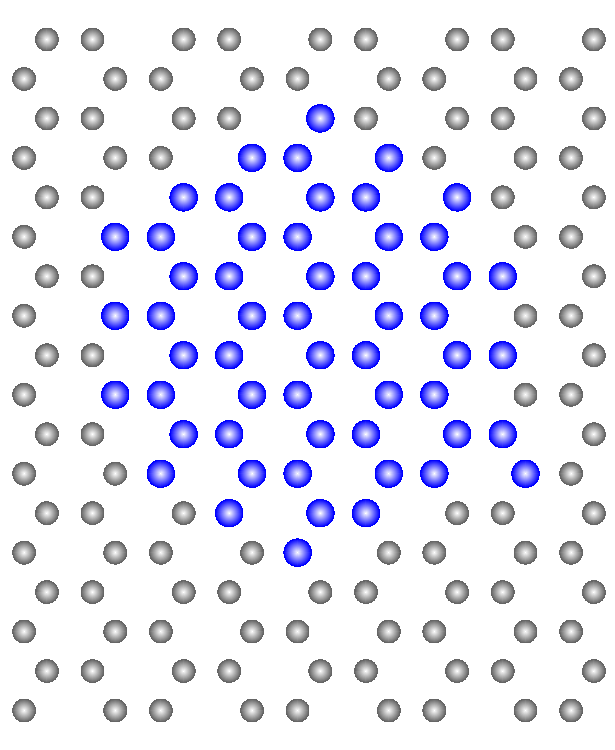
\includegraphics[width=\textwidth]{Abbildungen/C2X2.pdf}
			\subcaption{$\rm C_2X_2$}
			\label{C2X2-Insel}
		\end{minipage}
		\hfill
		\begin{minipage}[b]{0.24\textwidth}
			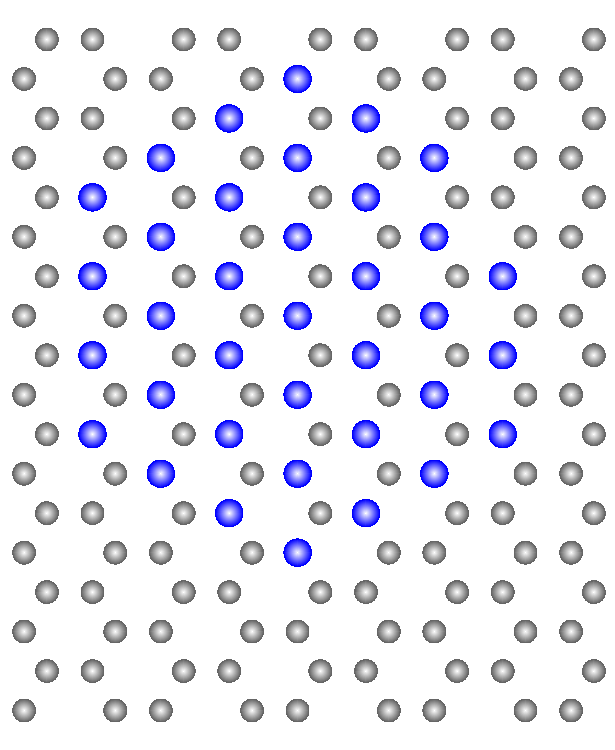
\includegraphics[width=\textwidth]{Abbildungen/C2X.pdf}
			\subcaption{$\rm C_2X$}
			\label{C2X-Insel}
		\end{minipage}
		\hfill
		\begin{minipage}[b]{0.24\textwidth}
			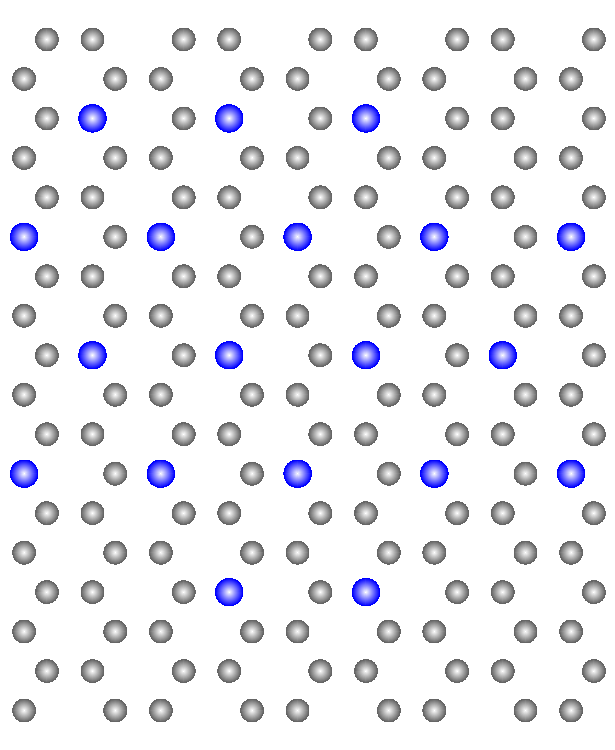
\includegraphics[width=\textwidth]{Abbildungen/C6X.pdf}
			\subcaption{$\rm C_6X$}
			\label{C6X-Insel}
		\end{minipage}
		\hfill
		\begin{minipage}[b]{0.24\textwidth}
			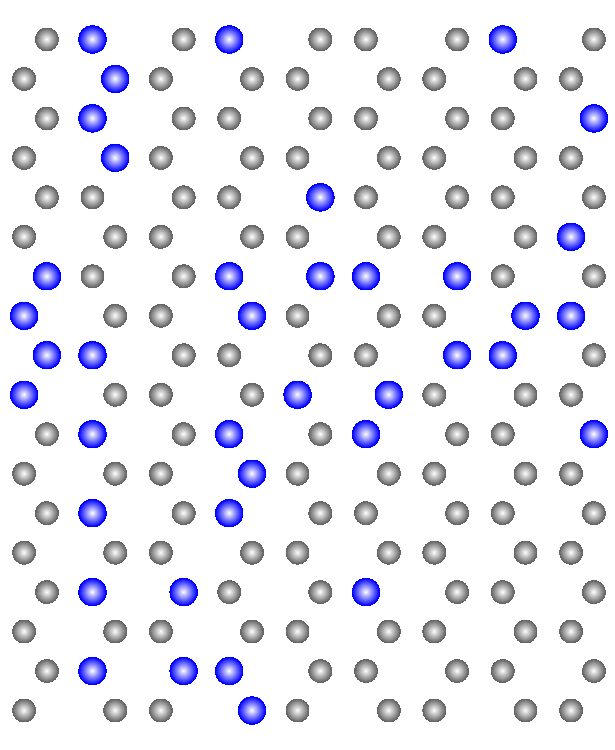
\includegraphics[width=\textwidth]{Abbildungen/random.pdf}
			\subcaption{ungeordnet}
			\label{ungeordnet}
		\end{minipage}
		\caption{Partielle Besetzung durch die vier Standardstrukturen}
		\label{Standardkonfigurationen}
	\end{figure}
	%
	Hier werden vier charakteristische Adsorbatkonfigurationen (siehe Abb.~\ref{Standardkonfigurationen}) vorgestellt, die aus den Berechnungen hervorgegangen sind. Mit Ausnahme der zufälligen Anordnungen handelt es sich dabei idealisiert um periodische Strukturen innerhalb von Bereichen, deren Größe durch die Adsorbatkonzentration $\cX$ beschränkt ist und außerhalb derer sich keine Fremdatome befinden. Tatsächlich gibt es aber immer wieder vereinzelte Ausreißer.
	
	Unter der Annahme, dass eine solche Struktur die gesamte Fläche bedeckt -- was jeweils nur bei einer einzigen Fremdatomanzahl möglich ist -- liegt dann wieder eine einfache Translationssymmetrie vor,\footnote{Bei Betrachtung einer Superzelle muss diese ein Vielfaches der neuen Elementarzelle darstellen, damit es nicht zu Antiphasengrenzen kommt. Siehe dazu Kap.~\ref{Startkonfiguration}.} so dass sich Bandschemata berechnen lassen. Aus diesen sind in einem beschränkten Rahmen auch Aussagen über teilbesetzte Systeme ableitbar, da sich das Energiespektrum beim Übergang von reinem Graphen zur Vollbesetzung fließend verändert.
	
	Darüber hinaus sollen die Strukturen auch mit Hilfe der im vorhergehenden Abschnitt vorgestellten Größen charakterisiert werden. Dies geschieht unter der Annahme einer idealen Insel, neben der keine isolierten Fremdatome existieren.
	
	\subsection{$\rm C_2X_2$-Inseln}
	
	Die $\rm C_2X_2$-Struktur (siehe Abb.~\ref{C2X2-Insel}) zeichnet sich durch die größtmögliche Adsorbatdichte aus, da sich bei jedem Kohlenstoff- ein Fremdatom befindet. Bei einem System mit $\cX = 1$ handelt es sich im Grunde um Graphan, nur dass der Aspekt der genauen räumlichen Anordnung der Fremdatome hier vernachlässigt wird.
	
	Die Elementarzellen von $\rm C_2X_2$ und reinem Graphen $\rm C_2$ sind identisch. Zur Berechnung der Eigenenergien muss man also nur die Matrix in Gl.~\ref{Energiematrix Graphen} um zwei Zeilen und Spalten für die beiden Fremdatome ergänzen. Man erhält
	%
	\begin{align*}
		\vec H =
		\begin{pmatrix}
            \eC         & z   &   V &  0 \\
            \overline z & \eC &   0 &  V \\
             V          & 0   & \eX &  0 \\
             0          & V   &   0 & \eX
		\end{pmatrix}.
	\end{align*}
	%
	Die vier Eigenwerte dieser Matrix lassen sich in die einfache analytische Form
	%
	\begin{figure}
		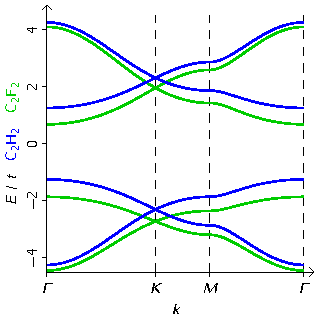
\includegraphics[width=0.48\textwidth]{Abbildungen/Bandstrukturen/C2X2.pdf}
		\hfill
		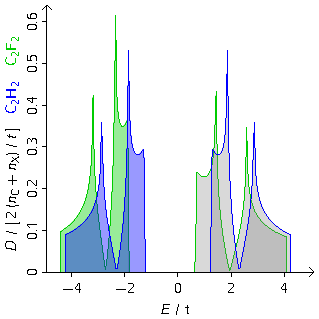
\includegraphics[width=0.48\textwidth]{Abbildungen/Bandstrukturen/DOS_C2X2.pdf}
		\caption{Bandstruktur und Zustandsdichte von $\rm C_2X_2$}
		\label{C2X2}
	\end{figure}
	%
	\begin{align*}
		E_{1, 2, 3, 4} = \frac 1 2 \bracks{E_\pm + \eX \pm \sqrt{4 V^2 + (E_\pm - \eX)^2}}
	\end{align*}
	%
	bringen, wobei $E_\pm$ die Bänder reinen Graphens beschreibt und dessen Vorzeichen als unabhängig von dem vor der Wurzel zu betrachten ist. Bandstruktur und Zustandsdichte sind in Abb.~\ref{C2X2} dargestellt. Ein markantes Merkmal ist die große Bandlücke im Bereich des \textsc{Fermi}-Niveaus. Bei Graphan handelt es sich also um einen Isolator. Zudem weist die Zustandsdichte für $\rm C_2F_2$ keine Spiegelsymmetrie auf im Gegensatz zu der für $\rm C_2H_2$, wo Elektronen- und Löcherdotierung äquivalent ist. Das gilt gleichermaßen für andere Adsorbatstrukturen.\footnote{siehe \cite[S. 3]{Wehling2}}
	
	Da die Gruppierung $G$ und die Kompaktheit $K$ sich ausschließlich auf direkte Nachbarschaft beziehen, sind sie zur Identifikation von $\rm C_2X_2$-Inseln besonders relevant. Während für eine einzelne Insel $G = 1$ ist, nimmt $K$ zwar stets große Werte an, kann aber erst für $\cX = 1$ maximal werden, wenn alle Randbereiche verschwunden sind. Davon unabhängig findet man die lokale Distanz $D = 1$. Weil die Fremdatome nicht in direkte Nachbarschaft miteinander treten und gleichzeitig eines beiden Untergitter bevorzugen können, ist schließlich die Polarisierung $P \approx 0$, die entsprechende Symmetrie also nicht gebrochen.
	
	\subsection{$\rm C_2X$-Inseln}
	
	Im Fall von $\rm C_2X$ (siehe Abb.~\ref{C2X-Insel}) befindet sich nur auf jedem zweiten Kohlenstoff- ein Fremdatom. Für $\cX > 0.5$ muss es daher innerhalb dieser Struktur unweigerlich zur Bildung von $\rm C_2X_2$-Inseln kommen. So hohe Adsorbatkonzentrationen werden in dieser Arbeit allerdings nicht betrachtet.
	
	Auch hier lässt sich zur Berechnung der Dispersion dieselbe Elementarzelle bedienen. Das führt etwa auf die Matrix
	%
	\begin{align*}
		\vec H =
		\begin{pmatrix}
			\eC         & z   & V \\
			\overline z & \eC & 0 \\
			V           & 0   & \eX
		\end{pmatrix}.
	\end{align*}
	%
	Obwohl diese kleiner ist als für $\rm C_2X_2$, bleibt die analytische Form der Eigenwerte nur für $\eC = \eX = 0$, d.h. Wasserstoffadsorbate, übersichtlich. Man findet
	%
	\begin{figure}
		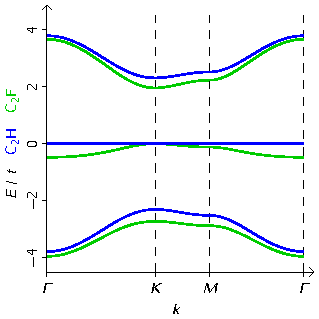
\includegraphics[width=0.48\textwidth]{Abbildungen/Bandstrukturen/C2X.pdf}
		\hfill
		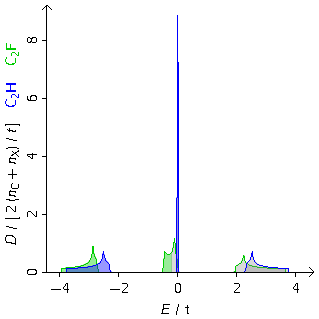
\includegraphics[width=0.48\textwidth]{Abbildungen/Bandstrukturen/DOS_C2X.pdf}
		\caption{Bandstruktur und Zustandsdichte von $\rm C_2X$}
		\label{C2X}
	\end{figure}
	%
	\begin{align*}
		E_1 = 0 \quad \text{und} \quad E_{2, 3} = \pm \sqrt{z^2 + V^2},
	\end{align*}
	%
	also betragsmäßig die geometrische Summe der Eigenenergie von Graphen und der \emph{hopping}-Energie $V$. Dass für jeden $\vec k$-Wert auch $E = 0$ ein Eigenwert ist, zeigt sich in der Zustandsdichte (siehe Abb.~\ref{C2X}) als einzelner hoher Peak. Für Fluor, also $\eX = -2\,\mathrm{eV}$ ist diese Entartung aufgehoben. Eine Bandlücke tritt sowohl unter- als auch oberhalb des \textsc{Fermi}-Niveaus auf.
	
	Da es hier keine direkt benachbarten Fremdatome gibt, ist $G = K = 0$. Zudem ist $D = 2$ und damit die Untergittersymmetrie vollständig gebrochen, d.h. $P = 1$.
	
	\subsection{$\rm C_6X$-Inseln}
	
	Durch erneutes Weglassen jedes zweiten Fremdatoms kommt man zur $\rm C_6X$-Struktur (siehe Abb.~\ref{C6X-Insel}). Deren Elementarzelle enthält nun 6 Kohlenstoffatome, weshalb eine vollbesetzte Struktur nur für eine Superzelle, deren Größe $l$ durch 3 teilbar ist, ohne einen Bruch der Translationssymmetrie möglich ist. Zwischenplätze müssen hier schon für $\cX > \nicefrac 1 6$ belegt werden.
	
	\begin{figure}
		\centering
		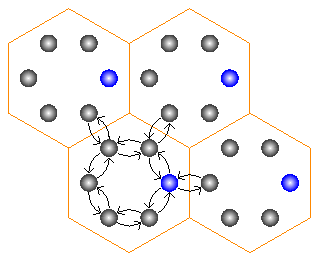
\includegraphics[width=0.48\textwidth]{Abbildungen/Raumstrukturen/Sechstel.pdf}
		\caption{Mögliche $t$-Übergänge in $\rm C_6X$ bzgl. einer Elementarzelle}
		\label{Uebergaenge C6X}
	\end{figure}
	%
	Eine geeignete Wahl ist die sechseckige Elementarzelle, die in Abb.~\ref{Uebergaenge C6X} mitsamt aller $t$-Übergänge dargestellt ist. Das \textsc{Bravais}-Gitter ist also wieder hexagonal, nur dass die Translationsvektoren die Länge $3 a$ aufweisen. Die angepassten Koordinaten $k_1$ und $k_2$ seien hier in Bezug auf das neue Gitter definiert. Eine mögliche Darstellung des \textsc{Hamilton}-Operators ist
	%
	\begin{figure}
		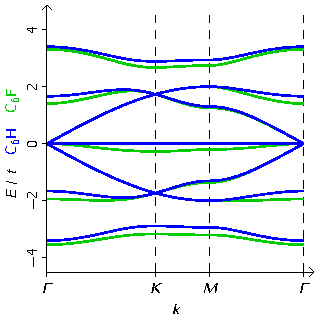
\includegraphics[width=0.48\textwidth]{Abbildungen/Bandstrukturen/C6X.pdf}
		\hfill
		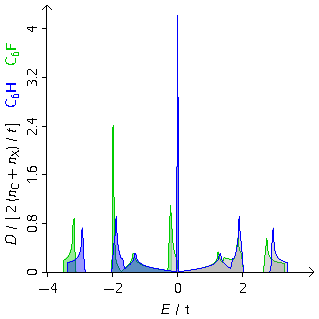
\includegraphics[width=0.48\textwidth]{Abbildungen/Bandstrukturen/DOS_C6X.pdf}
		\caption{Bandstruktur und Zustandsdichte von $\rm C_6X$}
		\label{C6X}
	\end{figure}
	%
	\begin{align*}
		\vec H =
		\begin{pmatrix}
	        \eC             & -t              &  0                     & -t \E^{\I k_1} &  0             & -t                     &  V \\
	        -t              & \eC             & -t                     &  0             & -t \E^{\I k_2} &  0                     &  0 \\
	         0              & -t              & \eC                    & -t             &  0             & -t \E^{\I (k_2 - k_1)} &  0 \\
	        -t \E^{-\I k_1} &  0              & -t                     & \eC            & -t             &  0                     &  0 \\
	         0              & -t \E^{-\I k_2} &  0                     & -t             & \eC            & -t                     &  0 \\
	        -t              &  0              & -t \E^{\I (k_1 - k_2)} &  0             & -t             & \eC                    &  0 \\
	         V              &  0              &  0                     &  0             &  0             &  0                     & \eX
		\end{pmatrix}.
	\end{align*}
	%
	Die sieben resultierenden Bänder werden hier nicht explizit in Formeln gefasst. In Abb.~\ref{C6X} sind sie mitsamt der Zustandsdichte grafisch dargestellt. Abb.~\ref{C6X Kontur} im Anhang zeigt zudem den Verlauf des Symmetriepfades über einer Konturdarstellung ausgewählter Bänder. Wie bei $\rm C_2X$ wird die Entartung für $E = 0$ bei Wasserstoff- für Fluorstrukturen aufgehoben. Es existieren des Weiteren zwei etwas schmalere Bandlücken beiderseits des \textsc{Fermi}-Niveaus.
	
	Die beschreibenden Größen liefern hier weitestgehend die gleichen Werte wie für die $\rm C_2X$-Struktur. Nur $D = 4$ passt sich dem neuen Fremdatomabstand an.
	
	\subsection{Ungeordnete Strukturen}
	
	Darüber hinaus gibt es auch Bereiche im Phasendiagramm, die sich keinem der oben genannten Fälle zuweisen lassen (siehe Abb.~\ref{ungeordnet}). Die Strukturen folgen dort keiner unmittelbar ersichtlichen Ordnung.
	
	Vom Begriff "`zufällig"' wird dennoch abgesehen, weil teilweise doch Regelmäßigkeiten erkennbar sind, etwa, wie gezeigt werden wird, eine kontinuierliche Veränderung der Kompaktheit $K$ innerhalb dieser Phase. Ferner nimmt $G$ sehr kleine Werte an, da es stets viele Fremdatome gibt, die keiner "`Gruppe"' zugehörig sind. Die Untergittersymmetrie ist auf Grund der Unordnung nicht gebrochen und daher $P \approx 0$.
	
	\section{Vollständige Betrachtung kleiner Systeme}
	\label{kleine Systeme}
	
	Für sehr kleine Systeme ist es im Rahmen einer überschaubaren Rechenzeit noch möglich das gesamte Ensemble von Mikrozuständen zu berücksichtigen. Das ermöglicht einem einen direkten Zugang zu globalen Minima der Energie, deren zugehörige Adsorbatstrukturen mit den Resultaten des Optimierungsalgorithmus verglichen werden können. Etwaige Unterschiede können dann entweder durch die Systemgröße bedingt, aber auch ein Zeichen dafür sein, dass der Algorithmus nicht über bestimmte lokale Minima hinauskommt.
	
	Betrachtet werden hier Superzellen der Größen $l = 3$ (dargestellt in Abb.~\ref{Orientierung}) bzw. $l = 6$, da das auch $\rm C_6X$-Strukturen die Möglichkeit zur periodischen Fortsetzung bietet. Während für $l = 3$ noch alle Adsorbatkonzentrationen ohne großen rechnerischen Aufwand untersucht werden können, beschränkt sich diese Arbeit für $l = 6$ auf $\nX = 4$ bzw. $\cE = \nicefrac 1 {18}$, da so bereits
	%
	\begin{align*}
		\binom \nC \nX = \frac{\nC!}{\nX! \ (\nC - \nX)!} = \frac{72!}{4! \ 68!} = 1 \, 028 \, 790
	\end{align*}
	%
	mögliche Kombinationen existieren, wobei sich ein Großteil durch Translationen oder Rotationen ineinander überführen ließe.\footnote{Vgl. die Binomialkoeffizienten $\binom {72} 5 = 13 \, 991 \, 544$ und $\binom {72} 6 = 156 \, 238 \, 908$.} Diese symmetrischen Äquivalenzen im vornherein zu identifizieren ist allerdings so aufwendig, dass es vorzuziehen ist eine wiederholte Berechnung entsprechender Energien in Kauf zu nehmen, vor allem weil diese auf Grund der kleinen Systemgröße sehr schnell vonstattengeht.
	
	\begin{figure}
		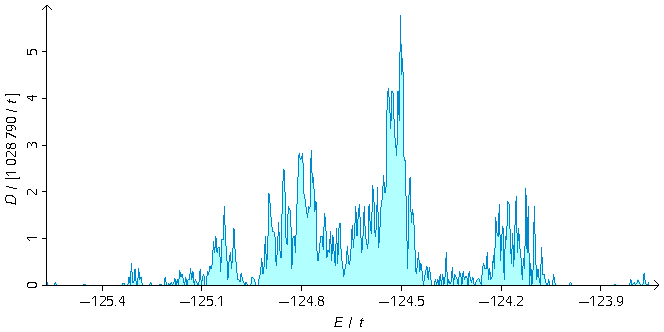
\includegraphics[width=\textwidth]{Abbildungen/Zustandsdichten/75.pdf}
		\caption[Ensemble-Dichte ohne Dotierung]{Ensemble-Dichte für ein undotiertes System aus 72 Kohlenstoff- und vier Fremdatomen.}
		\label{Phasenvolumen}
	\end{figure}
	%
	In Abb.~\ref{Phasenvolumen} (vgl. auch Abb.~\ref{Phasenvolumen2} im Anhang) ist die Zustandsdichte letzteren Ensembles für $\cE = 0$ dargestellt. Sie zeigt, dass die Anzahl der Realisierungsmöglichkeiten eines globalen Minimums im Vergleich zu anderen Energien verschwindend ist. Außerdem geht hervor, dass der energetische Spielraum, den die Variation der Adsorbatstruktur bietet, klein gegenüber dem Betrag der Energie ist. Die Kenntnis solcher Information könnte von Vorteil bei tiefergehender Beschäftigung mit dem \textsc{Metropolis}-Algorithmus oder Simulated Annealing sein.
	
	\section{Phasendiagramme}
	\label{Phasendiagramme}
	
	Jetzt soll der Blick weg von der genauen Beschaffenheit der unterschiedlichen Phasen und hin zu ihrer Lage in vollständigen Phasendiagrammen gerichtet werden.
	
	\begin{figure}
		\begin{minipage}[b]{0.48\textwidth}
			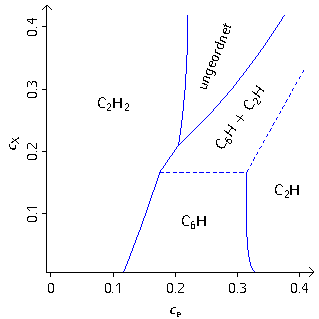
\includegraphics[width=\textwidth]{Abbildungen/Phasendiagramme/Schemata/H.pdf}
			\subcaption{Wasserstoffstrukturen ohne Penalty}
		\end{minipage}
		\hfill
		\begin{minipage}[b]{0.48\textwidth}
			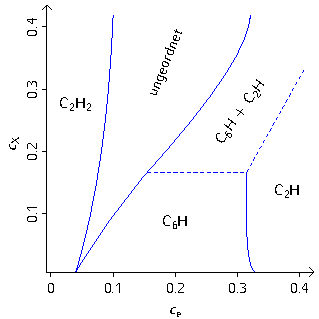
\includegraphics[width=\textwidth]{Abbildungen/Phasendiagramme/Schemata/H_penalty.pdf}
			\subcaption{Wasserstoffstrukturen mit Penalty}
		\end{minipage}
		
		\medskip
		
		\begin{minipage}[b]{0.48\textwidth}
			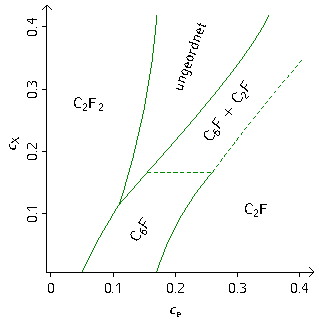
\includegraphics[width=\textwidth]{Abbildungen/Phasendiagramme/Schemata/F.pdf}
			\subcaption{Fluorstrukturen ohne Penalty}
		\end{minipage}
		\hfill
		\begin{minipage}[b]{0.48\textwidth}
			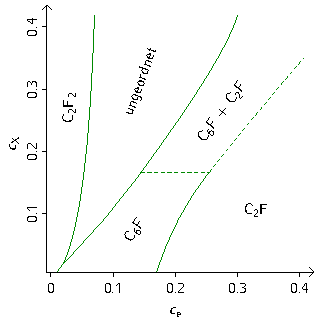
\includegraphics[width=\textwidth]{Abbildungen/Phasendiagramme/Schemata/F_penalty.pdf}
			\subcaption{Fluorstrukturen mit Penalty}
		\end{minipage}
		\caption[Präferenz einer der vier Standardkonfigurationen]{Schematische Phasendiagramme bzgl. der Präferenz einer der vier Standardkonfigurationen, berechnet an einer Superzelle der Größe $l = 18$. Die Phasengrenzen der Originalbilder, die eine Auflösung von $33 \times 33$ Bildpunkten hatten, wurden manuell nachgezeichnet.}
		\label{Schemata}
	\end{figure}
	%
	Dazu wird zunächst auch von einem Optimierungsalgorithmus abgesehen und für ausgewählte Punkte des Diagramms lediglich berechnet, welche der vier oben aufgeführten Standardkonfigurationen die energetisch günstigste ist. Das führt auf die in Abb.~\ref{Schemata} gezeigten Schemata, die einen groben Überblick über das Verhalten von Wasserstoff- und Fluoradsorbaten ohne und mit Penalty in einer Superzelle der Größe $l = 18$ liefern.
	
	Für die periodischen Strukturen werden dabei sechseckige Inseln oder auch \emph{"`Cluster"'} entsprechender Dichte und mit $\cE$ wachsender Größe angenommen, wobei $\rm C_6X$ nach Erreichen der Grenze $\cE = \nicefrac 1 6$ dem gleichen Schema folgend mit $\rm C_2X$ aufgefüllt wird. Die ungeordnete Struktur wird hier geäußerter Einwände zum Trotz durch eine komplett zufällige Anordnung der $\nX$ Fremdatome repräsentiert -- alles andere wäre willkürlich.
	
	Erst im zweiten Schritt werden Phasendiagramme mit Hilfe des Hill-Climbing-Algorithmus berechnet, und zwar für alle Kombinationen folgender drei Parameter: Als \emph{(i) Ausgangskonfigurationen} dienen neben $\rm C_2X_2$-Clustern zufällige sowie die oben berechneten für jeden Bildpunkt individuell günstigsten Strukturen. Des Weiteren kommen Wasserstoff und Fluor als \emph{(ii) Adsorbate} infrage und auch der Einfluss von \emph{(iii) Penalties} wird untersucht.
	
	Betrachtet wird eine Superzelle der Größe $l = 12$, was einerseits ein Kompromiss zwischen hinreichender Systemgröße und kurzen Rechenzeiten ist, und andererseits die Hoffnung weckt durch die große Teileranzahl möglichst vielen Strukturen einen passenden Rahmen zu geben.
	
	Die maximale Anzahl an Iterationen beträgt je $N = 2000$, wobei Schritte, die daran gescheitert sind, dass ein Zielkohlenstoffatom schon besetzt war, nicht mitgezählt werden. Nach $n = 100$ Schritten in Folge ohne eine Verbesserung der Energie wird angenommen, dass ein Minimum erreicht wurde, und die Schleife abgebrochen.
	
	Die Darstellung erfolgt dann für jede der beschreibenden Größen $G$, $K$, $D$ und $P$ separat. Es handelt sich um Abb.~\ref{H_G} bis \ref{F_P}, die im Anhang zu finden sind.
	
	\begin{figure}[b]
		\begin{minipage}[t]{0.31\textwidth}
			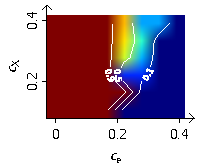
\includegraphics[width=\textwidth]{Abbildungen/Phasendiagramme/Exakt/H_G.pdf}
			\subcaption{Wasserstoff, Gruppierung}
			\label{HGx}
		\end{minipage}
		\hfill
		\begin{minipage}[t]{0.31\textwidth}
			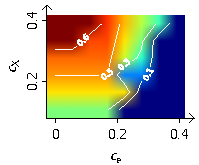
\includegraphics[width=\textwidth]{Abbildungen/Phasendiagramme/Exakt/H_K.pdf}
			\subcaption{Wasserstoff, Kompaktheit}
			\label{HKx}
		\end{minipage}
		\hfill
		\begin{minipage}[t]{0.31\textwidth}
			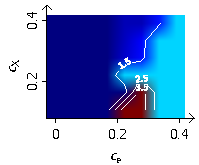
\includegraphics[width=\textwidth]{Abbildungen/Phasendiagramme/Exakt/H_D.pdf}
			\subcaption{Wasserstoff, lokale Distanz}
			\label{HDx}
		\end{minipage}
		
		\bigskip
		
		\begin{minipage}[t]{0.31\textwidth}
			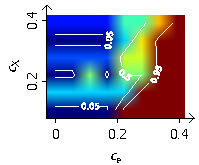
\includegraphics[width=\textwidth]{Abbildungen/Phasendiagramme/Exakt/H_P.pdf}
			\subcaption{Wasserstoff, Polarisierung}
			\label{HPx}
		\end{minipage}
		\hfill
		\parbox[b]{0.3\textwidth}{
			\caption[Phasendiagramme für globale Minima kleiner Systeme]{Phasendiagramme für eine Superzelle mit $l = 3$, wobei nur globale Energieminima verwendet wurden. Die Auflösung ist durch die diskrete Elektronenanzahl auf hier $8 \times 8$ Bildpunkte begrenzt. Adsorbatspezifische Unterschiede sind verschwindend.}
			\vspace{-1.5pc}
			\label{exakte Phasen}
			}
		\hfill
		\begin{minipage}[t]{0.31\textwidth}
			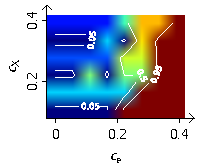
\includegraphics[width=\textwidth]{Abbildungen/Phasendiagramme/Exakt/F_P.pdf}
			\subcaption{Fluor, Polarisierung}
			\label{FPx}
		\end{minipage}
		
		\bigskip
		
		\begin{minipage}[t]{0.31\textwidth}
			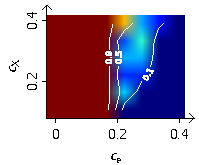
\includegraphics[width=\textwidth]{Abbildungen/Phasendiagramme/Exakt/F_G.pdf}
			\subcaption{Fluor, Gruppierung}
			\label{FGx}
		\end{minipage}
		\hfill
		\begin{minipage}[t]{0.31\textwidth}
			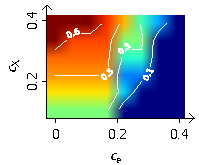
\includegraphics[width=\textwidth]{Abbildungen/Phasendiagramme/Exakt/F_K.pdf}
			\subcaption{Fluor, Kompaktheit}
			\label{FKx}
		\end{minipage}
		\hfill
		\begin{minipage}[t]{0.31\textwidth}
			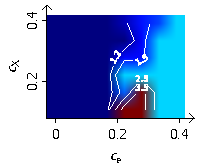
\includegraphics[width=\textwidth]{Abbildungen/Phasendiagramme/Exakt/F_D.pdf}
			\subcaption{Fluor, lokale Distanz}
			\label{FDx}
		\end{minipage}
	\end{figure}
	%
	Abschließend werden für eine kleine Superzelle mit $l = 3$ weitere Phasendiagramme für Wasserstoff- und Fluoradsorbate erzeugt (siehe Abb.~\ref{exakte Phasen}), in die nur tatsächliche globale Minima einfließen. Auf eine Analyse bzgl. der Strafenergie wird dabei verzichtet. Es zeigt sich, dass zumindest eine qualitative Übereinstimmung mit den bisherigen Ergebnissen besteht, sowohl in Bezug auf die Diagramme, als auch auf die zugrundeliegenden Strukturen.
	
	\subsection{Unterschiede zwischen Wasserstoff und Fluor}
	
	Die Phasendiagramme für Wasserstoff und Fluor auf Graphen unterscheiden sich weniger in Bezug auf die aufgetretenen Phasen, als auf die Verläufe ihrer Grenzen. Diese werden hier nur kurz beschrieben, ohne dabei Erklärungsversuche anzustellen.
	
	Abb.~\ref{Schemata} zeigt, dass der Übergang von $\rm C_2X_2$- zu ungeordneten oder $\rm C_6X$-Strukturen bei Fluor schon für geringere Elektronenzahlen auftritt. Außerdem ist auffällig, dass die $\rm C_6X$-Phase, die unterhalb der Winkelhalbierenden liegt und sich mit zunehmenden Teilchenkonzentrationen mit der $\rm C_2X$-Struktur vermischt -- das entspricht nicht nur der idealisierten Annahme, sondern auch den Hill-Climbing-Ergebnissen --, für Wasserstoff breiter ist.
	
	Allerdings scheint auch die Systemgröße hier eine Rolle zu spielen. So finden sich für das kleine exakt durchgerechnete System (siehe Abb.~\ref{exakte Phasen}) kaum Unterschiede zwischen den Phasendiagrammen für Wasserstoff- und Fluoradsorbate.
	
	\subsection{Einfluss der Startkonfiguration}
	\label{Startkonfiguration}
	
	Einen wesentlichen Einfluss auf das Resultat des Hill-Climbing-Algorithmus hat die Wahl der Ausgangskonfiguration. Das ist gleichbedeutend mit der Aussage, dass tatsächlich überwiegend lokale Minima gefunden werden, was nicht bedeutet, dass aus diesen keine Tendenzen der Adsorbate bestimmte Ordnungen herzustellen ableitbar sind.
	
	Als Beispiel diene ein zufällig gewählter Ausgangszustand für einen Punkt im Phasendiagramm, an dem die Bildung von Clustern bevorzugt ist. Zu Beginn der Optimierung werden sich lokal viele kleinere Ansammlungen von Fremdatomen bilden: ein Vorgang der die Energie des Systems unmittelbar senkt. Um diese dann allerdings zu einem großen Cluster zusammenzuführen müssten sich viele Fremdatome simultan in eine bestimmte Richtung bewegen können, was die hier gewählte Art der Variation nicht zulässt. Es könnte immer nur ein einzelnes Atom einen Schritt in Richtung eines anderen Clusters vollziehen, was dessen kurzzeitige Absonderung vom eigenen implizieren und damit die Energie erhöhen würde. Vergleichbares wird für $T = 0$ aber nicht akzeptiert. Es bleibt also bei kleineren Fremdatomansammlungen oder -ketten, auch wenn diese energetisch nicht optimal sind.
	
	Dieser Effekt ist die Ursache dafür, dass in Abb.~\ref{H_random_G} und \ref{H_penalty_random_G} sowie \ref{F_random_G} und \ref{F_penalty_random_G} verhältnismäßig geringe Werte für die Gruppierung $G$ zu finden sind. Umgekehrt ist es einfacher einen bereits existierenden Cluster zu "`sprengen"' wie aus Abb.~\ref{H_cluster_G} und \ref{H_penalty_cluster_G} sowie \ref{F_cluster_G} und \ref{F_penalty_cluster_G} hervorgeht: Für hohe $\cE$ bleibt vom ursprünglichen Cluster nicht viel zurück.
	
	Analog lassen sich auch \emph{Antiphasengrenzen} erklären, also Linien beideseits derer \emph{Domänen} gleicher periodische Struktur vorliegen, die allerdings so gegeneinander verschoben sind, dass sie nicht nahtlos ineinander übergehen.\footnote{\emph{"`An antiphase boundary is an interface within a crystal across which there is a mistake in the translational symmetry."'} \cite[S. 218f]{Putnis}} Das kann trotz lokalem Bruch der Untergittersymmetrie zu einer globalen Polarisierung $P \approx 0$ führen. Entsprechendes gilt natürlich auch für Bereiche, die nicht direkt benachbart sind.
	
	Phänomene dieser Art begründen wiederum die starken Unregelmäßigkeiten der Polarisierung unterhalb der Winkelhalbierenden in Abb.~\ref{H_cluster_P} bis \ref{H_penalty_random_P} sowie \ref{F_cluster_P} bis \ref{F_penalty_random_P}.
	
	Durch die Wahl individuell günstiger Ausgangskonfigurationen kann dergleichen effizient unterbunden werden. In Abb.~\ref{H_G} bis \ref{F_P} zeigt sich, dass die Phasengrenzen in (e) und (f) im Vergleich zu denen in (a) bis (d) überwiegend sehr scharf gezeichnet sind. Dadurch, dass man \emph{a priori} sehr viele Informationen und vermutlich auch lokale Minima mit einfließen lässt, wird die Wirkung des Hill-Climbing-Algorithmus also vermindert.
	
	\subsection{Auswirkungen von Penalties}
	
	Da die Einführung von Penalties sich gegen die direkte Nachbarschaft von Fremdatomen richtet, ist eine mit ihr einhergehende Verkleinerung der Bereiche im Phasendiagramm zu erwarten, in denen diese prävalent ist. Tatsächlich findet man neben einer allgemein erhöhten Anzahl an Fremdatomen, die keiner Gruppe zuordenbar sind, eine entsprechende Verschiebung der $\rm C_2X_2$-Phasengrenze.
	
	Sie kommt der $\cX$-Achse nun wesentlich näher (siehe Abb.~\ref{Schemata}), und zwar insbesondere im Bereich kleiner $\cX$, wo sich die $\rm C_6X$-Phase fast bis zum Ursprung ausgeweitet hat (siehe Abb.~\ref{H_D} und \ref{F_D}). Dieser Effekt ist für Wasserstoff deutlicher zu erkennen als für Fluor, da die $C_2F_2$-Phase ohnehin schwächer ausgeprägt ist.
	
	Wie u.a. der Verlauf der Kompaktheit in Abb.~\ref{H_K} und \ref{F_K} zeigt, sind Fremdatomnachbarschaften nun fast ausschließlich auf die Hälfte des Phasendiagramms oberhalb der Winkelhalbierenden beschränkt, während dem entgegengesetzt in der gesamten unteren Hälfte ein Bruch der Untergittersymmetrie günstig zu sein scheint, wie aus Abb.~\ref{H_P} und \ref{F_P} hervorgeht. Im Folgenden wird unter anderem dieser Phasenübergang diskutiert.
	
	\section{Klassifizierung ausgewählter Phasenübergänge}
	\label{Klassifizierung ausgewaehlter Phasenuebergaenge}
	
	\subsection{$\rm C_2X_2 \rightarrow C_6X \rightarrow C_2X$}
	
	\begin{figure}
		\begin{minipage}[t]{0.48\textwidth}
			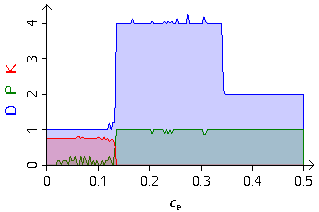
\includegraphics[width=\textwidth]{Abbildungen/C2X2-C6X-C2X.pdf}
			\subcaption{Verlauf für Superzelle mit $l = 12$, also $\nC = 288$ und $\nX = 16$. Die Optimierung individueller Ausgangskonfigurationen wurde nach $n = 300$ erfolglosen oder max. $N = 3000$ Schritten abgebrochen.}
		\end{minipage}
		\hfill
		\begin{minipage}[t]{0.48\textwidth}
			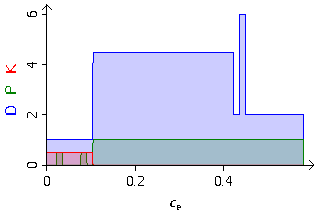
\includegraphics[width=\textwidth]{Abbildungen/C2X2-C6X-C2X-exact.pdf}
			\subcaption{Entsprechender Verlauf unter ausschließlicher Einbeziehung globaler Minima für eine Superzelle mit $l = 6$, also $\nC = 72$ und $\nX = 4$.}
		\end{minipage}
		\caption[Der Übergang $\rm C_2X_2 \rightarrow C_6X \rightarrow C_2X$]{Lokale Distanz, Polarisierung und Kompaktheit für den Übergang $\rm C_2X_2 \rightarrow C_6X \rightarrow C_2X$ bei $\cX = \nicefrac 1 {18} = 0.0\overline5$. Die horizontale Auflösung ist durch gequantelte Elektronenanzahl beschränkt.}
		\label{Phasenuebergaenge1}
	\end{figure}
	%
	\begin{figure}
		\begin{minipage}[b]{0.19\textwidth}
			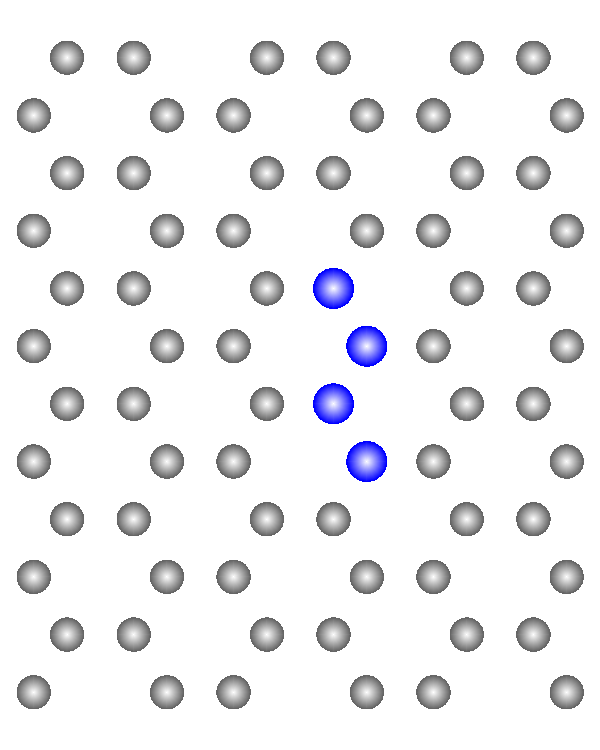
\includegraphics[width=\textwidth]{Abbildungen/ne83.pdf}
			\subcaption{$\nE = 83$}
		\end{minipage}
		\hfill
		\begin{minipage}[b]{0.19\textwidth}
			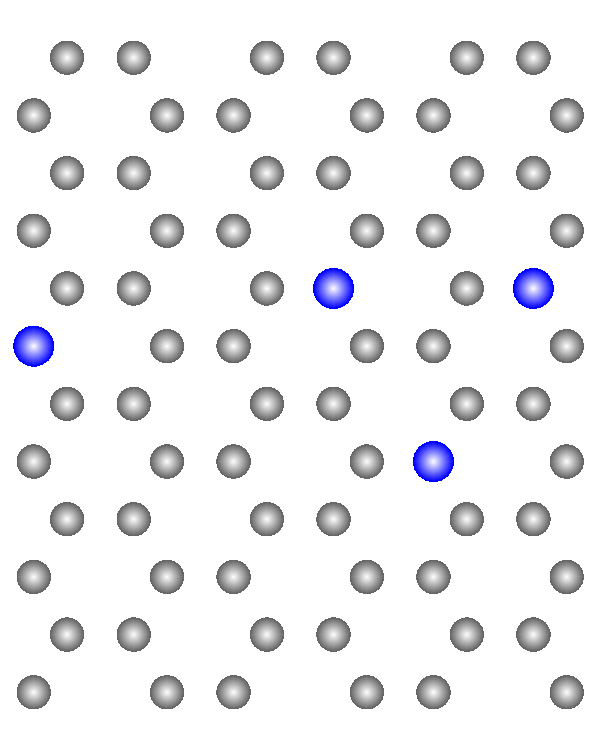
\includegraphics[width=\textwidth]{Abbildungen/ne84.pdf}
			\subcaption{$\nE = 84$}
		\end{minipage}
		\hfill
		\begin{minipage}[b]{0.19\textwidth}
			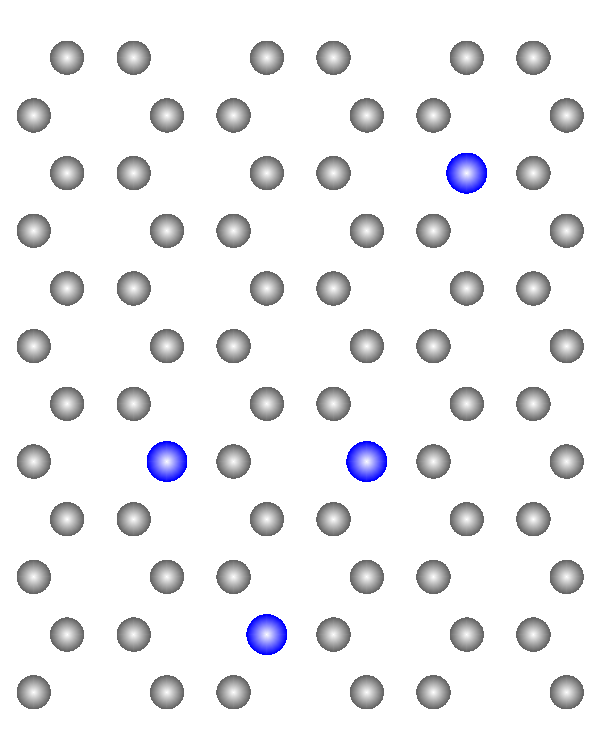
\includegraphics[width=\textwidth]{Abbildungen/ne106.pdf}
			\subcaption{$\nE = 106$}
		\end{minipage}
		\hfill
		\begin{minipage}[b]{0.19\textwidth}
			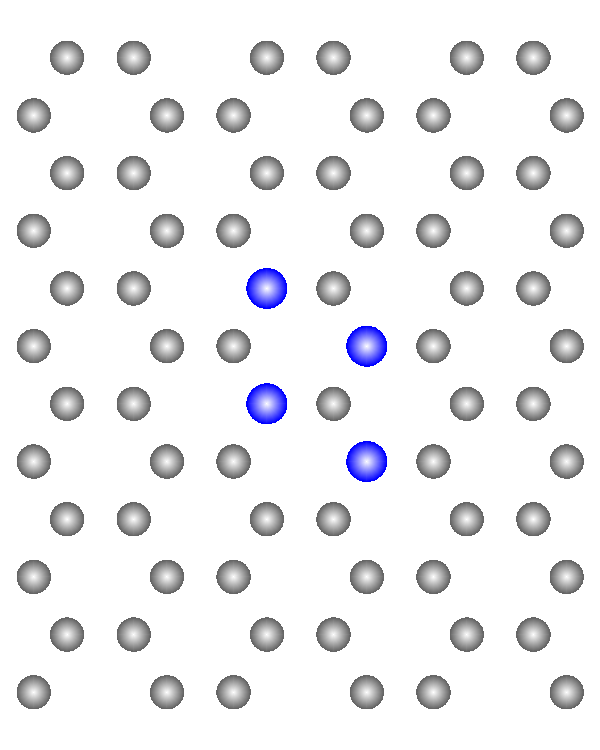
\includegraphics[width=\textwidth]{Abbildungen/ne107.pdf}
			\subcaption{$\nE = 107$}
		\end{minipage}
		\hfill
		\begin{minipage}[b]{0.19\textwidth}
			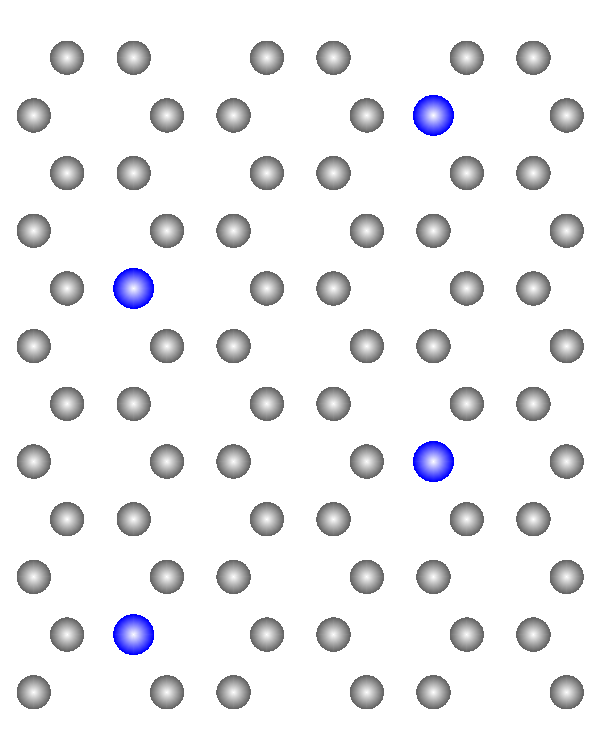
\includegraphics[width=\textwidth]{Abbildungen/ne108.pdf}
			\subcaption{$\nE = 108$}
		\end{minipage}
		\caption[Konfigurationen globaler Energieminima]{Konfigurationen globaler Energieminima für Wasserstoffadsorbate ohne Penalty unmittelbar vor und nach den Phasenübergängen $\rm C_2X_2 \rightarrow \rm C_6X$ (a, b) und $\rm C_6X \rightarrow C_2X$ (c, d) sowie ein Ausnahmezustand (e). Neben einer $\rm C_6X$-Insel befindet sich jeweils ein isoliertes Fremdatom.}
		\label{Phasenvergleich exakt}
	\end{figure}
	%
	Von der Ausdehnung der $\rm C_2X_2$-Phase abgesehen zeigt sich also, dass die Untergittersymmetrie für $\cE \gtrsim \cX$, also unterhalb der Winkelhalbierenden, gebrochen ist.\footnote{in Übereinstimmung mit \cite[S. 1]{Wehling2}: \emph{"`\emph{[\dots]}, charge doping is shown to trigger a sublattice ordering transition when the doping level exceeds the adsorbate concentration."'}} Diesen Bereich teilen sich wiederum die $\rm C_6X$- und die $\rm C_2X$-Struktur. Um den exakten Verlauf der Phasen und Übergänge verfolgen zu können wird ein hochaufgelöster horizontaler Schnitt durch den untereren Bereich des Phasendiagramms für Wasserstoffadsorbate ohne Penalty untersucht, d.h. bei konstantem $\cX = \nicefrac 1 {18}$ ein Minimum für jedes mögliche $\nE$ innerhalb des betrachteten $\cE$-Intervalls bestimmt und beschrieben.
	
	Dabei wird erneut die Superzelle der Größe $l = 12$ betrachtet. Es werden individuelle Ausgangskonfigurationen verwendet, denn wenn im Bereich des Phasenübergangs Abweichungen von diesen schon sehr günstigen Strukturen auftreten, gibt das zumindest die Gewissheit, dass man es nicht mit einem vollständig diskontinuierlichen Übergang zu tun hat. Umgekehrt kann man von einer clusterförmigen oder zufälligen Anordnung ausgehend nicht einmal innerhalb einer Phase damit rechnen, dass die beschreibenden Größen einen annähernd kontinuierlichen Verlauf zeigen. Die Optimierung wird nach $n = 300$ erfolglosen bzw. maximal nach $N = 3000$ Schritten abgebrochen.
	
	Um abschätzen zu können, ob die Ergebnisse zumindest qualitativ zutreffend sind, werden wieder globale Minima kleiner Systeme hinzugezogen, hier der bereits diskutierten Superzelle aus $72$ Kohlenstoff- und vier Fremdatomen (siehe Kap.~\ref{kleine Systeme}). Ein Vergleich der Übergänge, die sich aus beiden Ansätzen ergeben, ermöglicht Abb.~\ref{Phasenuebergaenge1}.
	
	Insbesondere die exakten Rechnung legen nahe, dass tatsächlich so etwas wie strukturelle Phasenübergänge erster Ordnung bzgl. der Kompaktheit, der Polarisierung und der lokalen Distanz vorliegen, wobei sich der zweite Übergang nur in letzterer niederschlägt. Zwischen den Unstetigkeiten bleiben die beschreibenden Größen konstant.
	
	Abb.~\ref{Phasenvergleich exakt} zeigt die Konfigurationen des kleinen Systems unmittelbar vor und nach den beiden Übergängen, sowie die Ursache für den $D = 6$-Peak innerhalb der $\rm C_2X$-Phase. Es fällt auf, dass keine perfekten $\rm C_6X$-Inseln zustande gekommen sind, sondern nur dreiecksförmige Anordnungen, an der das jeweils vierte Fremdatom keinen Anteil hat. Die Auffälligkeiten der Polarisierung innerhalb der $\rm C_2X_2$-Phase sind der kleinen Systemgröße verschuldet: Ordnen sich drei der Fremdatome in unmittelbarer Nachbarschaft um das vierte an, sind die beiden Untergitter bereits im Verhältnis 3:1 besetzt.
	
	Des Weiteren sind im großen System tatsächlich nur geringe Veränderungen der individuell vorgegebenen Strukturen festzustellen, die sich in Form punktueller Abweichungen von den sonst konstanten Werten zeigen. Dabei handelt es sich stets um einzelne sich absondernde Fremdatome. Während ihre Abstände vom Rest unmittelbar vor und nach der $\rm C_6X$-Phase deren lokaler Distanz entsprechen, was dem Phasenübergang doch eine verschwindende Kontinuität verleiht, ist dazwischen, wie auch im kleinen System, die Existenz eines isoliertes Fremdatoms vom Übergang unabhängig energetisch günstig.
	
	\subsection{Von $\rm C_2X_2$-Inseln zu ungeordneten Strukturen}
	
	\begin{figure}[b]
		\begin{minipage}[t]{0.48\textwidth}
			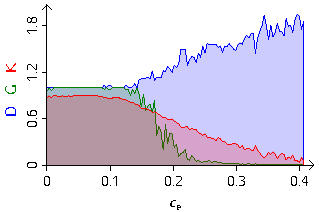
\includegraphics[width=\textwidth]{Abbildungen/C2X2-random.pdf}
			\subcaption{Verlauf für die Superzelle der Größe $l = 12$, also $\nC =~288$ und $\nX = 96$. Die "`Sprengung"' anfänglicher Cluster wurde hier erst nach $n = 500$ bzw. $N = 5000$ Schritten abgebrochen.}
		\end{minipage}
		\hfill
		\begin{minipage}[t]{0.48\textwidth}
			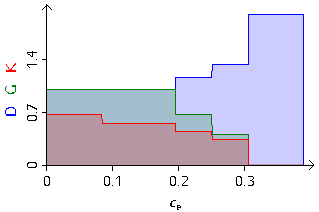
\includegraphics[width=\textwidth]{Abbildungen/C2X2-random-exact.pdf}
			\subcaption{Entsprechender Verlauf unter ausschließlicher Einbeziehung globaler Minima für eine Superzelle mit $l = 3$, also $\nC = 18$ und $\nX = 6$.}
		\end{minipage}
		\caption[Der Übergang von $\rm C_2X_2$ in die ungeordnete Phase]{Lokale Distanz, Gruppierung und Kompaktheit für den Übergang von $\rm C_2X_2$ in die ungeordnete Phase bei $\cX = \nicefrac 1 3$. Auch hier ist die horizontale Auflösung durch die Elektronen beschränkt.}
		\label{Phasenuebergaenge2}
	\end{figure}
	%
	Analog wird auch der Übergang von der $\rm C_2X_2$- in die ungeordnete Phase im oberen Bereich des Phasendiagramms, genauer bei $\cX = \nicefrac 1 3$, analysiert, von dem aus vorigen Rechnungen (siehe z.B. Abb.~\ref{H_K}) bereits bekannt ist, dass er sich fließend über einen größeren Bereich erstreckt. Deshalb wird hier auch ausschließlich eine $\rm C_2X_2$-Insel als Ausgangspunkt genommen und dafür die Schrittanzahl auf $N = 500$ bzw. $n = 5000$ erhöht.
	
	Dem Vergleich dient hier das bereits durchgerechnete System der Größe $l = 3$ (siehe Abb.~\ref{exakte Phasen}) Er wird in Abb.~\ref{Phasenuebergaenge2} vollzogen.
	
	Sowohl der Hill-Climbing-Algorithmus, als auch die exakte Rechnung offenbaren kontinuierliche Verläufe der lokalen Distanz, der Gruppierung uns insbesondere der Kompaktheit, die hier den erwähnten äußerst sanften Abfall zeigt. Innerhalb der ungeordneten Phase scheinen die Fremdatome also dafür Sorge zu tragen, dass eine bestimmte Anzahl direkter Nachbarschaften gewährleistet ist. Insgesamt kann man durchaus von kontinuierlichen und somit Phasenübergängen zweiter Ordnung sprechen.
	
	\chapter{Zusammenfassung und Ausblick}
	
	Für ein einfaches Tight-Binding-Modell von Graphen mit Wasserstoff- bzw. Fluoradsorbaten konnte bestätigt werden, dass in Abhängigkeit der Ladungsträger- und Fremdatomkonzentrationen bestimmte Adsorbatstrukturen energetisch günstiger sind als andere.
	
	Diese wurden auf zweierlei Weise berechnet: Zum einen wurde ein Optimierungs-, genauer der Hill-Climbing-Algorithmus verwendet, bei dem man den Vorteil auch größere Systeme mit überschaubarem Rechenaufwand untersuchen zu können mit dem Risiko bezahlt lediglich lokale Minima zu finden. Zum anderen konnten auch tatsächliche globale Minima durch Berechnung vollständiger Zustandsensembles gefunden werden, allerdings nur für sehr kleine Systeme. Beide Ansätze führten zu ähnlichen Ergebnisse.
	
	Insgesamt wurden vier verschiedene Phasen identifiziert: Bei dreien handelt es sich idealisiert um Inseln periodischer Strukturen -- namentlich $\rm C_2X_2$, $\rm C_6X$ und $\rm C_2X$, wobei die Fremdatome stets äquidistant angeordnet sind --, umgeben von reinem Graphen. Für diese wurden unter der Annahme einer Vollbesetzung, d.h. für die reine, lückenlose Struktur, elektronische Bandschemata und Zustandsdichten berechnet, die allerdings nur oberflächlich diskutiert wurden. Hier könnte man unter Umständen auch auf experimentellem Weg anknüpfen, etwa über Messungen der Leitfähigkeit. Die vierte Phase hingegen weist keine augenscheinliche Ordnung auf, auch diesbezüglich könnten weitere Nachforschungen angestellt werden.
	
	Um sich über subjektive Beobachtungen hinaus auch auf quantitative Werte stützen zu können, wurden des Weiteren vier Größen zur Beschreibung von Adsorbatkonfigurationen definiert: die Gruppiertheit, die Kompaktheit, die lokale Distanz sowie die Polarisierung. Alle beschreiben die Lage der Fremdatome zueinander, legen aber dabei aber verschiedene Schwerpunkte.
	
	Es hat sich zudem gezeigt, dass zwischen den Phasen teils kontinuierliche, teils diskontinuierliche strukturelle Übergänge existieren. Diese Beobachtung wurde sowohl durch die heuristische, als auch die exakte Methode bestätigt.
	
	Schließlich wurde auch noch der Einfluss einer Variation verschiedener Systemparameter untersucht. Im Wesentlichen findet man, dass durch die Wahl des Adsorbatelements oder die Einführung von Straftermen zwar die Phasengrenzen verschoben, die Phasen selbst aber nur geringfügig beinflusst werden. In Bezug auf letztere war hingegen die Ausgangskonfiguration des Optimierungsalgorithmus ausschlaggebend, doch auch diese konnte über die grundlegenden Tendenzen nicht hinwegtäuschen.
	
	Zusammenfassend wurde in dieser Arbeit also hauptsächlich dahingehend geforscht, welche Arten von Phänomenen im System "`Fremdatome auf dotiertem Graphen"' qualitativ überhaupt zu erwarten sind. Um verlässlichere Voraussagen machen zu können müssten also weitere Aspekte integriert werden, wie etwa die genaue räumliche Anordnung der Atome zueinander oder auch thermische Effekte. Aber selbst im Rahmen des verwendeten Modells wurde die Frage nach den Ursachen für die gefundenen Strukturen weitestgehend offengelassen. Um diesbezüglich Antworten zu finden müsste den Zusammenhängen zwischen ausgewählten Merkmalen in der elektronischen und der räumlichen Struktur detaillierter nachgegangen werden. Auch welche anwendungsbezogenen Materialeigenschaften sich mit Hilfe vergleichbarer Erkenntnisse erzielen lassen, bleibt hier noch unbeantwortet.
	
	\appendix
	
	\chapter{Abbildungen}
	
	\begin{figure}
		\begin{minipage}[t]{0.48\textwidth}
			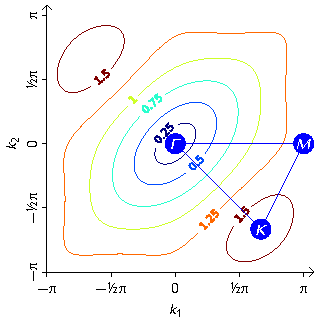
\includegraphics[width=\textwidth]{Abbildungen/Bandstrukturen/BZ_C6X_4.pdf}
			\subcaption{drittgrößte Eigenenergien}
		\end{minipage}
		\hfill
		\begin{minipage}[t]{0.48\textwidth}
			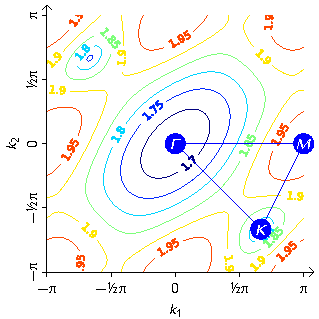
\includegraphics[width=\textwidth]{Abbildungen/Bandstrukturen/BZ_C6X_5.pdf}
			\subcaption{zweitgrößte Eigenenergien}
		\end{minipage}
		\caption[Konturdarstellung der Dispersionsrelation von $\rm C_6X$]{Konturdarstellung der strukturreichsten Bänder von $\rm C_6X$ und Lage des Symmetriepfads.}
		\label{C6X Kontur}
	\end{figure}
	%
	\begin{figure}
		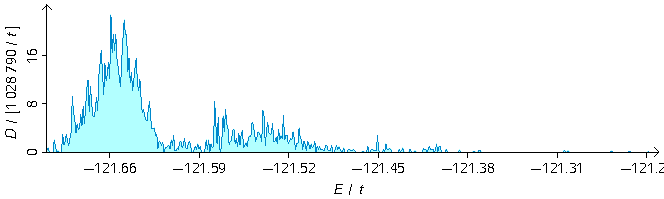
\includegraphics[width=\textwidth]{Abbildungen/Zustandsdichten/84.pdf}
		\caption[Ensemble-Dichte mit Dotierung]{Ensemble-Dichte für System aus 72 Kohlenstoff- und vier Fremdatomen sowie $\cE = 0.125$, d.h. 9 Dotierungselektronen. Sie ist durch die Dotierung stark zu kleineren Energien hin verschoben.}
		\label{Phasenvolumen2}
	\end{figure}
	%
	Im Folgenden sind weitere Abbildungen zu finden, die im Laufe dieser Arbeit erwähnt wurden. Insbesondere handelt es sich dabei um die Phasendiagramme, die mit Hilfe des Hill-Climbing-Algorithmus für alle Kombinationen der Ausgangskonfiguration ($\rm C_2X_2$-Insel, zufällig oder individuell) der Adsorbatsorte (Wasserstoff oder Fluor) sowie der Strafenergie $p \in \braces{0, 0.5\,\mathrm{eV}}$ für eine Superzelle der Größe $l = 12$ berechnet wurden, wobei die Optimierung nach 100 erfolglosen oder maximal 2000 Schritten abgebrochen wurde.
	
	\begin{figure}
		\begin{minipage}[t]{0.48\textwidth}
			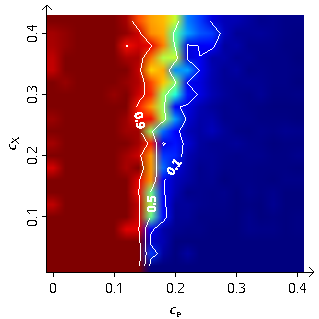
\includegraphics[width=\textwidth]{Abbildungen/Phasendiagramme/Konturen/H_cluster_G.pdf}
			\subcaption{$\rm C_2H_2$-Inseln, $p = 0$}
			\label{H_cluster_G}
		\end{minipage}
		\hfill
		\begin{minipage}[t]{0.48\textwidth}
			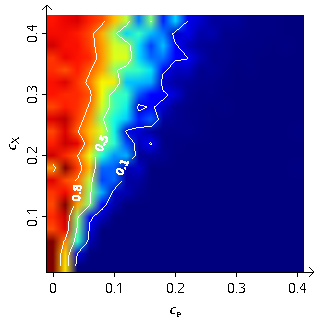
\includegraphics[width=\textwidth]{Abbildungen/Phasendiagramme/Konturen/H_penalty_cluster_G.pdf}
			\subcaption{$\rm C_2H_2$-Inseln, $p = 0.5\,\mathrm{eV}$}
			\label{H_penalty_cluster_G}
		\end{minipage}
		%
		\begin{minipage}[t]{0.48\textwidth}
			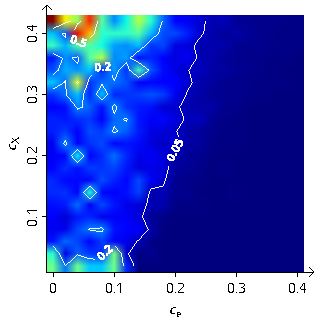
\includegraphics[width=\textwidth]{Abbildungen/Phasendiagramme/Konturen/H_random_G.pdf}
			\subcaption{zufällig, $p = 0$}
			\label{H_random_G}
		\end{minipage}
		\hfill
		\begin{minipage}[t]{0.48\textwidth}
			\includegraphics[width=\textwidth]{Abbildungen/Phasendiagramme/Konturen/H_penalty_random_G.pdf}
			\subcaption{zufällig, $p = 0.5\,\mathrm{eV}$}
			\label{H_penalty_random_G}
		\end{minipage}
		%
		\begin{minipage}[t]{0.48\textwidth}
			\includegraphics[width=\textwidth]{Abbildungen/Phasendiagramme/Konturen/H_individual_G.pdf}
			\subcaption{individuell, $p = 0$}
			\label{H_individual_G}
		\end{minipage}
		\hfill
		\begin{minipage}[t]{0.48\textwidth}
			\includegraphics[width=\textwidth]{Abbildungen/Phasendiagramme/Konturen/H_penalty_individual_G.pdf}
			\subcaption{individuell, $p = 0.5\,\mathrm{eV}$}
			\label{H_penalty_individual_G}
		\end{minipage}
		\caption[Gruppierung finaler Wasserstoffstrukturen]{Gruppierung finaler Wasserstoffstrukturen für verschiedene Startkonfigurationen}
		\label{H_G}
	\end{figure}
	
	\begin{figure}
		\begin{minipage}[t]{0.48\textwidth}
			\includegraphics[width=\textwidth]{Abbildungen/Phasendiagramme/Konturen/H_cluster_K.pdf}
			\subcaption{$\rm C_2H_2$-Inseln, $p = 0$}
			\label{H_cluster_K}
		\end{minipage}
		\hfill
		\begin{minipage}[t]{0.48\textwidth}
			\includegraphics[width=\textwidth]{Abbildungen/Phasendiagramme/Konturen/H_penalty_cluster_K.pdf}
			\subcaption{$\rm C_2H_2$-Inseln, $p = 0.5\,\mathrm{eV}$}
			\label{H_penalty_cluster_K}
		\end{minipage}
		%
		\begin{minipage}[t]{0.48\textwidth}
			\includegraphics[width=\textwidth]{Abbildungen/Phasendiagramme/Konturen/H_random_K.pdf}
			\subcaption{zufällig, $p = 0$}
			\label{H_random_K}
		\end{minipage}
		\hfill
		\begin{minipage}[t]{0.48\textwidth}
			\includegraphics[width=\textwidth]{Abbildungen/Phasendiagramme/Konturen/H_penalty_random_K.pdf}
			\subcaption{zufällig, $p = 0.5\,\mathrm{eV}$}
			\label{H_penalty_random_K}
		\end{minipage}
		%
		\begin{minipage}[t]{0.48\textwidth}
			\includegraphics[width=\textwidth]{Abbildungen/Phasendiagramme/Konturen/H_individual_K.pdf}
			\subcaption{individuell, $p = 0$}
			\label{H_individual_K}
		\end{minipage}
		\hfill
		\begin{minipage}[t]{0.48\textwidth}
			\includegraphics[width=\textwidth]{Abbildungen/Phasendiagramme/Konturen/H_penalty_individual_K.pdf}
			\subcaption{individuell, $p = 0.5\,\mathrm{eV}$}
			\label{H_penalty_individual_K}
		\end{minipage}
		\caption[Kompaktheit finaler Wasserstoffstrukturen]{Kompaktheit finaler Wasserstoffstrukturen für verschiedene Startkonfigurationen}
		\label{H_K}
	\end{figure}
	
	\begin{figure}
		\begin{minipage}[t]{0.48\textwidth}
			\includegraphics[width=\textwidth]{Abbildungen/Phasendiagramme/Konturen/H_cluster_D.pdf}
			\subcaption{$\rm C_2H_2$-Inseln, $p = 0$}
			\label{H_cluster_D}
		\end{minipage}
		\hfill
		\begin{minipage}[t]{0.48\textwidth}
			\includegraphics[width=\textwidth]{Abbildungen/Phasendiagramme/Konturen/H_penalty_cluster_D.pdf}
			\subcaption{$\rm C_2H_2$-Inseln, $p = 0.5\,\mathrm{eV}$}
			\label{H_penalty_cluster_D}
		\end{minipage}
		%
		\begin{minipage}[t]{0.48\textwidth}
			\includegraphics[width=\textwidth]{Abbildungen/Phasendiagramme/Konturen/H_random_D.pdf}
			\subcaption{zufällig, $p = 0$}
			\label{H_random_D}
		\end{minipage}
		\hfill
		\begin{minipage}[t]{0.48\textwidth}
			\includegraphics[width=\textwidth]{Abbildungen/Phasendiagramme/Konturen/H_penalty_random_D.pdf}
			\subcaption{zufällig, $p = 0.5\,\mathrm{eV}$}
			\label{H_penalty_random_D}
		\end{minipage}
		%
		\begin{minipage}[t]{0.48\textwidth}
			\includegraphics[width=\textwidth]{Abbildungen/Phasendiagramme/Konturen/H_individual_D.pdf}
			\subcaption{individuell, $p = 0$}
			\label{H_individual_D}
		\end{minipage}
		\hfill
		\begin{minipage}[t]{0.48\textwidth}
			\includegraphics[width=\textwidth]{Abbildungen/Phasendiagramme/Konturen/H_penalty_individual_D.pdf}
			\subcaption{individuell, $p = 0.5\,\mathrm{eV}$}
			\label{H_penalty_individual_D}
		\end{minipage}
		\caption[Lokale Distanz finaler Wasserstoffstrukturen]{Lokale Distanz finaler Wasserstoffstrukturen für verschiedene Startkonfigurationen}
		\label{H_D}
	\end{figure}
	
	\begin{figure}
		\begin{minipage}[t]{0.48\textwidth}
			\includegraphics[width=\textwidth]{Abbildungen/Phasendiagramme/Konturen/H_cluster_P.pdf}
			\subcaption{$\rm C_2H_2$-Inseln, $p = 0$}
			\label{H_cluster_P}
		\end{minipage}
		\hfill
		\begin{minipage}[t]{0.48\textwidth}
			\includegraphics[width=\textwidth]{Abbildungen/Phasendiagramme/Konturen/H_penalty_cluster_P.pdf}
			\subcaption{$\rm C_2H_2$-Inseln, $p = 0.5\,\mathrm{eV}$}
			\label{H_penalty_cluster_P}
		\end{minipage}
		%
		\begin{minipage}[t]{0.48\textwidth}
			\includegraphics[width=\textwidth]{Abbildungen/Phasendiagramme/Konturen/H_random_P.pdf}
			\subcaption{zufällig, $p = 0$}
			\label{H_random_P}
		\end{minipage}
		\hfill
		\begin{minipage}[t]{0.48\textwidth}
			\includegraphics[width=\textwidth]{Abbildungen/Phasendiagramme/Konturen/H_penalty_random_P.pdf}
			\subcaption{zufällig, $p = 0.5\,\mathrm{eV}$}
			\label{H_penalty_random_P}
		\end{minipage}
		%
		\begin{minipage}[t]{0.48\textwidth}
			\includegraphics[width=\textwidth]{Abbildungen/Phasendiagramme/Konturen/H_individual_P.pdf}
			\subcaption{individuell, $p = 0$}
			\label{H_individual_P}
		\end{minipage}
		\hfill
		\begin{minipage}[t]{0.48\textwidth}
			\includegraphics[width=\textwidth]{Abbildungen/Phasendiagramme/Konturen/H_penalty_individual_P.pdf}
			\subcaption{individuell, $p = 0.5\,\mathrm{eV}$}
			\label{H_penalty_individual_P}
		\end{minipage}
		\caption[Polarisierung finaler Wasserstoffstrukturen]{Polarisierung finaler Wasserstoffstrukturen für verschiedene Startkonfigurationen}
		\label{H_P}
	\end{figure}
	
	\begin{figure}
		\begin{minipage}[t]{0.48\textwidth}
			\includegraphics[width=\textwidth]{Abbildungen/Phasendiagramme/Konturen/F_cluster_G.pdf}
			\subcaption{$\rm C_2F_2$-Inseln, $p = 0$}
			\label{F_cluster_G}
		\end{minipage}
		\hfill
		\begin{minipage}[t]{0.48\textwidth}
			\includegraphics[width=\textwidth]{Abbildungen/Phasendiagramme/Konturen/F_penalty_cluster_G.pdf}
			\subcaption{$\rm C_2F_2$-Inseln, $p = 0.5\,\mathrm{eV}$}
			\label{F_penalty_cluster_G}
		\end{minipage}
		%
		\begin{minipage}[t]{0.48\textwidth}
			\includegraphics[width=\textwidth]{Abbildungen/Phasendiagramme/Konturen/F_random_G.pdf}
			\subcaption{zufällig, $p = 0$}
			\label{F_random_G}
		\end{minipage}
		\hfill
		\begin{minipage}[t]{0.48\textwidth}
			\includegraphics[width=\textwidth]{Abbildungen/Phasendiagramme/Konturen/F_penalty_random_G.pdf}
			\subcaption{zufällig, $p = 0.5\,\mathrm{eV}$}
			\label{F_penalty_random_G}
		\end{minipage}
		%
		\begin{minipage}[t]{0.48\textwidth}
			\includegraphics[width=\textwidth]{Abbildungen/Phasendiagramme/Konturen/F_individual_G.pdf}
			\subcaption{individuell, $p = 0$}
			\label{F_individual_G}
		\end{minipage}
		\hfill
		\begin{minipage}[t]{0.48\textwidth}
			\includegraphics[width=\textwidth]{Abbildungen/Phasendiagramme/Konturen/F_penalty_individual_G.pdf}
			\subcaption{individuell, $p = 0.5\,\mathrm{eV}$}
			\label{F_penalty_individual_G}
		\end{minipage}
		\caption[Gruppierung finaler Fluorstrukturen]{Gruppierung finaler Fluorstrukturen für verschiedene Startkonfigurationen}
		\label{F_G}
	\end{figure}
	
	\begin{figure}
		\begin{minipage}[t]{0.48\textwidth}
			\includegraphics[width=\textwidth]{Abbildungen/Phasendiagramme/Konturen/F_cluster_K.pdf}
			\subcaption{$\rm C_2F_2$-Inseln, $p = 0$}
			\label{F_cluster_K}
		\end{minipage}
		\hfill
		\begin{minipage}[t]{0.48\textwidth}
			\includegraphics[width=\textwidth]{Abbildungen/Phasendiagramme/Konturen/F_penalty_cluster_K.pdf}
			\subcaption{$\rm C_2F_2$-Inseln, $p = 0.5\,\mathrm{eV}$}
			\label{F_penalty_cluster_K}
		\end{minipage}
		%
		\begin{minipage}[t]{0.48\textwidth}
			\includegraphics[width=\textwidth]{Abbildungen/Phasendiagramme/Konturen/F_random_K.pdf}
			\subcaption{zufällig, $p = 0$}
			\label{F_random_K}
		\end{minipage}
		\hfill
		\begin{minipage}[t]{0.48\textwidth}
			\includegraphics[width=\textwidth]{Abbildungen/Phasendiagramme/Konturen/F_penalty_random_K.pdf}
			\subcaption{zufällig, $p = 0.5\,\mathrm{eV}$}
			\label{F_penalty_random_K}
		\end{minipage}
		%
		\begin{minipage}[t]{0.48\textwidth}
			\includegraphics[width=\textwidth]{Abbildungen/Phasendiagramme/Konturen/F_individual_K.pdf}
			\subcaption{individuell, $p = 0$}
			\label{F_individual_K}
		\end{minipage}
		\hfill
		\begin{minipage}[t]{0.48\textwidth}
			\includegraphics[width=\textwidth]{Abbildungen/Phasendiagramme/Konturen/F_penalty_individual_K.pdf}
			\subcaption{individuell, $p = 0.5\,\mathrm{eV}$}
			\label{F_penalty_individual_K}
		\end{minipage}
		\caption[Kompaktheit finaler Fluorstrukturen]{Kompaktheit finaler Fluorstrukturen für verschiedene Startkonfigurationen}
		\label{F_K}
	\end{figure}
	
	\begin{figure}
		\begin{minipage}[t]{0.48\textwidth}
			\includegraphics[width=\textwidth]{Abbildungen/Phasendiagramme/Konturen/F_cluster_D.pdf}
			\subcaption{$\rm C_2F_2$-Inseln, $p = 0$}
			\label{F_cluster_D}
		\end{minipage}
		\hfill
		\begin{minipage}[t]{0.48\textwidth}
			\includegraphics[width=\textwidth]{Abbildungen/Phasendiagramme/Konturen/F_penalty_cluster_D.pdf}
			\subcaption{$\rm C_2F_2$-Inseln, $p = 0.5\,\mathrm{eV}$}
			\label{F_penalty_cluster_D}
		\end{minipage}
		%
		\begin{minipage}[t]{0.48\textwidth}
			\includegraphics[width=\textwidth]{Abbildungen/Phasendiagramme/Konturen/F_random_D.pdf}
			\subcaption{zufällig, $p = 0$}
			\label{F_random_D}
		\end{minipage}
		\hfill
		\begin{minipage}[t]{0.48\textwidth}
			\includegraphics[width=\textwidth]{Abbildungen/Phasendiagramme/Konturen/F_penalty_random_D.pdf}
			\subcaption{zufällig, $p = 0.5\,\mathrm{eV}$}
			\label{F_penalty_random_D}
		\end{minipage}
		%
		\begin{minipage}[t]{0.48\textwidth}
			\includegraphics[width=\textwidth]{Abbildungen/Phasendiagramme/Konturen/F_individual_D.pdf}
			\subcaption{individuell, $p = 0$}
			\label{F_individual_D}
		\end{minipage}
		\hfill
		\begin{minipage}[t]{0.48\textwidth}
			\includegraphics[width=\textwidth]{Abbildungen/Phasendiagramme/Konturen/F_penalty_individual_D.pdf}
			\subcaption{individuell, $p = 0.5\,\mathrm{eV}$}
			\label{F_penalty_individual_D}
		\end{minipage}
		\caption[Lokale Distanz finaler Fluorstrukturen]{Lokale Distanz finaler Fluorstrukturen für verschiedene Startkonfigurationen}
		\label{F_D}
	\end{figure}
	
	\begin{figure}
		\begin{minipage}[t]{0.48\textwidth}
			\includegraphics[width=\textwidth]{Abbildungen/Phasendiagramme/Konturen/F_cluster_P.pdf}
			\subcaption{$\rm C_2F_2$-Inseln, $p = 0$}
			\label{F_cluster_P}
		\end{minipage}
		\hfill
		\begin{minipage}[t]{0.48\textwidth}
			\includegraphics[width=\textwidth]{Abbildungen/Phasendiagramme/Konturen/F_penalty_cluster_P.pdf}
			\subcaption{$\rm C_2F_2$-Inseln, $p = 0.5\,\mathrm{eV}$}
			\label{F_penalty_cluster_P}
		\end{minipage}
		%
		\begin{minipage}[t]{0.48\textwidth}
			\includegraphics[width=\textwidth]{Abbildungen/Phasendiagramme/Konturen/F_random_P.pdf}
			\subcaption{zufällig, $p = 0$}
			\label{F_random_P}
		\end{minipage}
		\hfill
		\begin{minipage}[t]{0.48\textwidth}
			\includegraphics[width=\textwidth]{Abbildungen/Phasendiagramme/Konturen/F_penalty_random_P.pdf}
			\subcaption{zufällig, $p = 0.5\,\mathrm{eV}$}
			\label{F_penalty_random_P}
		\end{minipage}
		%
		\begin{minipage}[t]{0.48\textwidth}
			\includegraphics[width=\textwidth]{Abbildungen/Phasendiagramme/Konturen/F_individual_P.pdf}
			\subcaption{individuell, $p = 0$}
			\label{F_individual_P}
		\end{minipage}
		\hfill
		\begin{minipage}[t]{0.48\textwidth}
			\includegraphics[width=\textwidth]{Abbildungen/Phasendiagramme/Konturen/F_penalty_individual_P.pdf}
			\subcaption{individuell, $p = 0.5\,\mathrm{eV}$}
			\label{F_penalty_individual_P}
		\end{minipage}
		\caption[Polarisierung finaler Fluorstrukturen]{Polarisierung finaler Fluorstrukturen für verschiedene Startkonfigurationen}
		\label{F_P}
	\end{figure}
	
	\chapter{Quelltexte}
	
	Zur Ermittlung der vorgestellten Daten wurde ein Programm mit Benutzeroberfläche entwickelt, das eine einfache Eingabe von Adsorbatkonfigurationen erlaubt sowie Zustandsdichten und Phasendiagramme unmittelbar darstellt (\url{http://berges.canopus.uberspace.de/graphene}). Die Quelltexte der wichtigsten Komponenten werden in diesem Kapitel kommentiert dargestellt.
	
	Kernstück der Berechnungen ist das \emph{Python}-Skript \emph{graphene.py}, das die für die spezielle Problemstellung wichtigsten Subroutinen und Klassen bereitstellt. Es wird unter anderem vom \emph{CGI}-Skript \emph{index.py} verwendet, das über das \emph{Common Gateway Interface} die Kommunikation mit einem Webserver regelt. Die grafische Ausgabe erfolgt dann mittels der \emph{Hypertext Markup Language (HTML)}, \emph{Scalable Vector Graphics (SVG)} und \emph{Cascading Style Sheets (CSS)} im Webbrowser, wobei dynamische Elemente und Animationen durch das \emph{JavaScript} \emph{script.js} realisiert werden.
	
	Ferner sind das HTML-Template \emph{structure.html} und das Python-Modul \emph{graphics.py} zur Generierung der SVG-Plots involviert, die hier aber nicht vorgestellt werden.
	
	\section{graphene.py}
	
	\lstinputlisting[language = Python, firstline = 4]{Programm/graphene.py}
	
	\section{index.py}
	
	\lstinputlisting[language = Python, firstline = 4]{Programm/index.py}
	
	\section{script.js}
	
	\lstinputlisting[language = JavaScript]{Programm/script.js}
	
	\backmatter
	
	\vspace*{2cm}
	
	\begin{center}
		\begin{minipage}{0.67\textwidth}
			\chapter{Danksagung}
	
			Mein Dank gilt Prof. Dr. Tim Wehling für die Möglichkeit eine Bachelorarbeit über dieses spannende Thema schreiben zu dürfen, Dr. Bálint Aradi für das Zweitgutachten, Dr. Stefan Barthel für die Betreuung meiner Arbeit, letzterem, Alexander Schulz und Miriam Nüß für das Korrekturlesen, Christian Renk für Softwareempfehlungen, generell der gesamten Arbeitsgruppe für die freundliche Aufnahme, nicht zuletzt meinen Eltern für die Unterstützung meines Studiums sowie allen Entwickler/innen frei zugänglicher Software und Information.
		\end{minipage}
	\end{center}
	
	\chapter{Erklärungen}
	
	\bigskip
	
	\begin{flushright}
		\begin{tabular}{r l}
			\textbf{Name} & Jan Berges \\
			\textbf{Matrikelnummer} & 2727142
		\end{tabular}
	\end{flushright}
	
	\bigskip
	
	\section*{Urheberrechtliche Erklärung}

	\subsubsection*{Erklärung gem. \S 10 (10) Allgemeiner Teil der BPO vom 27.10.2010}
	
	Hiermit versichere ich, dass ich meine Bachelorarbeit ohne fremde Hilfe angefertigt habe, und dass ich keine anderen als die von mir angegebenen Quellen und Hilfsmittel benutzt habe.
	
	Alle Stellen, die wörtlich oder sinngemäß aus Veröffentlichungen entnommen sind, habe ich unter Angabe der Quellen als solche kenntlich gemacht.

	Die Bachelorarbeit darf nach Abgabe nicht mehr verändert werden.
	
	\vspace{1cm}

	\begin{flushright}
		Bremen, 4. September 2014
	\end{flushright}
	
	\vspace{1cm}
	
	\section*{Erklärung zur Veröffentlichung von Abschlussarbeiten}

	Ich bin damit einverstanden, dass meine Abschlussarbeit im Universitätsarchiv für wissenschaftliche Zwecke von Dritten eingesehen werden darf.
	
	Ich bin damit einverstanden, dass meine Abschlussarbeit nach 30 Jahren (gem. \S 7 Abs.~2 \mbox{BremArchivG}) im Universitätsarchiv für wissenschaftliche Zwecke von Dritten eingesehen werden darf.
	
	Ich bin damit einverstanden, dass meine Abschlussarbeit im Universitätsarchiv für wissenschaftliche Zwecke von Dritten eingesehen werden darf.
	
	\vspace{1cm}
	
	\begin{flushright}
		Bremen, 4. September 2014
	\end{flushright}
	
	\addcontentsline{toc}{chapter}{Abbildungsverzeichnis}
	\listoffigures
	
	\addcontentsline{toc}{chapter}{Literaturverzeichnis}

\begin{thebibliography}{\hspace{1cm}}
    \src{Ash}{Ashcroft}{N. W. Ashcroft, N. D. Mermin}{Solid State Physics}{Harcourt, Inc., 1976}
    \src{Big}{Biggs}{N. L. Biggs, E. K. Lloyd, R. J. Wilson}{Graph Theory 1736 -- 1936}{Oxford University Press, 1998}
    \src{Bor}{Born}{M. Born, R. Oppenheimer}{Zur Quantentheorie der Molekeln}{Annalen der Physik, Vol. 389, 1927}
    \src{Blo}{Bloch}{F. Bloch}{Über die Quantenmechanik der Elektronen in Kristallgittern}{Zeitschrift für Physik, Vol. 52, 1929}
    \src{Cór}{Cordoba}{A. Córdoba}{Dirac Combs}{Letters in Mathematical Physics, Vol. 17, Nr. 3, 1989}
    \src{Czy}{Czycholl}{G. Czycholl}{Theoretische Festkörperphysik. Von den klassischen Modellen zu modernen Forschungsthemen}{Springer-Verlag, Berlin/Heidelberg, 2008}
    \src{Dir}{Dirac}{P. A. M. Dirac}{The Principles of Quantum Mechanics}{Forth edition, revised. Oxford University Press, 1958}
    \src{Ede}{Edelsbrunner}{Herbert Edelsbrunner}{A Short Course in Computational Geometry and Topology}{Springer 2014}
    \src{Ehr1}{Ehrenfest1}{P. u. T. Ehrenfest}{Begriffliche Grundlagen der statistischen Auffassung in der Mechanik}{Encyklopädie der mathematischen Wissenschaften mit Einschluss ihrer Anwendungen, Band 4, Artikel 32, Leipzig, 1909 –- 1911}
    \src{Ehr2}{Ehrenfest2}{P. Ehrenfest}{Phasenumwandlungen im üeblichen und erweiterten Sinn, classifiziert nach den entsprechenden Singuaritaeten des thermodynamischen Potentiales}{Supplement Nr. 75b zu den Mitteilungen aus dem Kamerlingh Onnes-Institut, Leiden, 1933}
    \src[et al.]{Eli}{Elias}{D. C. Elias}{Control of Graphene's Properties by Reversible Hydrogenation: Evidence for Graphane}{Science, Vol. 323, Januar 2009}
    \src{Fli}{Fliessbach}{T. Fließbach}{Lehrbuch zur Theoretischen Physik IV: Statistische Physik}{5. Auflage, Spektrum Akademischer Verlag Heidelberg, 2010}
    \src{Hov}{vanHove}{Léon van Hove}{The Occurrence of Singularities in the Elastic Frequency Distribution of a Cristal}{Physical Review, Vol. 89, Nr. 6, 1953}
    \src{Jel}{Jelitto}{R. J. Jelitto}{Theoretische Physik 6: Thermodynamik und Statistik}{Aula-Verlag, 1985}
    \src{Kat1}{Katsnelson1}{M. I. Katsnelson}{Graphene: Carbon in Two Dimensions}{Erstauflage, Cambridge University Press, 2012}
    \src{Kat2}{Katsnelson2}{M. I. Katsnelson}{Graphene: Carbon in Two Dimensions}{Materials Today, Vol. 10, Nr. 1 -- 2, 2007}
    \src[et al.]{Kir}{Kirkpatrick}{S. Kirkpatrick}{Optimization by Simulated Annealing}{Science, New Series, Vol. 220, 1983}
    \src{Laa}{vanLaarhoven}{P. J. M. van Laarhoven, E. H. L. Aarts}{Simulated Annealing: Theory and Applications}{Springer Science+Business Media Dordrecht, 1987}
    \src{Lan1}{Landau1}{L. D. Landau}{On the Theory of Superconductivity \emph{(1937) in} Collected Papers of L. D. Landau \emph{von D. ter Haar}}{Erstausgabe, Gordon and Breach, Sience Publishers, 1965}
    \src{Lan2}{Landau2}{L. D. Landau, E. M. Lifshitz}{Course of Theoretical Physics, Vol. 5: Statistical Phyics, Pt. 1}{Third edition, revised and enlarged, Pergamon Press, 1980}
    \src{Mar}{Markov}{A. A. Markov}{An Example of Statistical Investigation of the Text Eugene Onegin Concerning the Connection of Samples in Chains}{Übersetzung: David Link. Science in Context 19.4, 2006, S. 591 -- 600}
    \src{Met1}{Metropolis1}{N. Metropolis, S. Ulam}{The Monte Carlo Method}{Journal of the American Statistical Association, Vol. 44, 1949}
    \src[et al.]{Met2}{Metropolis2}{N. Metropolis}{Equation of State Calculations by Fast Computing Machines}{The Journal of Chemical Physics, Vol. 21, 1953}
    \src{Nan}{Nandkishore}{R. Nandkishore}{Chiral superconductivity from repulsive interactions in doped graphene}{Nature Physics, Vol. 8, 2012}
    \src{Nol}{Nolting}{W. Nolting}{Grundkurs Theoretische Physik 6: Statistische Physik}{7. Auflage, Springer-Verlag Berlin, 2014}
    \src[et al.]{Nov1}{Novoselov1}{K. S. Novoselov}{Electric Field Effect in Atomically Thin Carbon Films}{Science, Vol. 306, Oktober 2004}
    \src{Nov2}{Novoselov2}{K. S. Novoselov}{Graphene: Materials in the Flatland}{Nobelpreisrede, 2010}
    \src{Pau}{Pauli}{W. Pauli}{Über den Zusammenhang des Abschlusses der Elektronengruppen im Atom mit der Komplexstruktur der Spektren}{Zeitschrift für Physik, Vol. 31, Nr. 1, 1925}
    \src{Put}{Putnis}{A. Putnis}{Introduction to mineral siences}{Cambridge University Press, 2003}
    \src{Roz}{Rozplocha}{F. Rozp\l{}ocha, J. Patyka, J. Stankowski}{Graphenes Bonding Forces in Graphite}{Acta Physica Polonica A, Vol. 112, 2007}
    \src{Sel}{Selman}{B. Selman, C. P. Gomes}{Hill Climbing Search}{Nature Encyclopedia of Cognition}
    \src{Set}{Sethna}{J. P. Sethna}{Order Parameters, Broken Symmetry, and Topology}{Lectures in Complex Systems, Eds. L. Nagel and D. Stein, Santa Fe, 1991}
    \src{Sch}{Schmidt}{J. A. E. Schmidt}{Griechisch-deutsches Handwörterbuch}{Leipzig 1827}
    \src{Tol}{Tolman}{R. C. Tolman}{The Principles of Statistical Mechanics}{Oxford University (Clarendon) Press, 1938}
    \src{Weh1}{Wehling1}{T. O. Wehling, M. I. Katsnelson, A. I. Lichtenstein}{First-principles studies of water adsorption on graphene: The role of the substrate}{Applied Physics Letters, Vol. 93, 2008}
    \src[et al.]{Weh2}{Wehling2}{T. O. Wehling}{Charge doping induced phase transitions in hydrogenated and fluorinated graphene}{Physical Review B, Vol. 90, August 2014}
\end{thebibliography}

	
\end{document}
